
%%% Local Variables:
%%% mode: latex
%%% TeX-master: slide.tex
%%% End:
\documentclass{beamerthemeMono}

% specify some optional logos
\graphicspath{{figures/}}
%\pgfdeclareimage[height=1.45cm]{mainlogo}{figures/logo}
\pgfdeclareimage[height=1.4cm]{mainlogo}{figures/Rlogo.png}
% placed in the lower left/right corner if the \pgfuseimage{minilogo}
% command is uncommented in the \institute command below.
\pgfdeclareimage[height=1cm]{minilogo}{figures/Rlogo.png}
\logo{\pgfuseimage{minilogo}}

\AtBeginSection[] {
  \begin{frame}
    \frametitle{目录} 
    {\tableofcontents[%
      currentsection, % causes all sections but the current to be shown in a semi-transparent way.
%     currentsubsection, % causes all subsections but the current subsection in the current section to ...
      hideallsubsections % causes all subsections to be hidden.
%     hideothersubsections, % causes the subsections of sections other than the current one to be hidden.
%     part=, % part number causes the table of contents of part part number to be shown
%     pausesections, % causes a \pause command to be issued before each section. This is useful if you
%     pausesubsections, %  causes a \pause command to be issued before each subsection.
%     sections={ overlay specification },
      ]}
   \end{frame}}

% \AtBeginSubsection[]                            % 在每个子段落之前
% {
%   \frame{                                         % handout:0 表示只在手稿中出现
%     \frametitle{目录} \small
%     \tableofcontents[
%       currentsection,
%       currentsubsection,
%       subsectionstyle=show/shaded/hide]
%   }
% }
%%%%%%%%%%%%%%%%%%%%%%%%%%%%%%%%%%%%%%%%%%%%%%%%%%%%%%%%%%%%
%%%%%%%%%%%%%%%%%%%%%%%%%%%%%%%%%%%%%%%%%%%%%%%%%%%%%%%%%%%%
          % 文档开始
%%%%%%%%%%%%%%%%%%%%%%%%%%%%%%%%%%%%%%%%%%%%%%%%%%%%%%%%%%%%
%%%%%%%%%%%%%%%%%%%%%%%%%%%%%%%%%%%%%%%%%%%%%%%%%%%%%%%%%%%%

\begin{document}

\title[现代统计图形及在R中的实现]% optional, use only with long paper titles
{\heiti \xiaoerhao 现代统计图形及在R中的实现}


\author[邹海翔] % optional, use only with lots of authors
{\xiaosihao 邹海翔}
\date{\xiaosihao 2018年 5 月}
 % - Give the names in the same order as they appear in the paper.  -
 % Use the \inst{?} command only if the authors have different
 % affiliation. See the beamer manual for an example


\institute[深圳市规划国土发展研究中心] % optional - is placed in the bottom of the sidebar on every slide
{%
   \xiaosihao 深圳市规划国土发展研究中心
   % there must be an empty line above this line - otherwise some
   % unwanted space is added
   % between the university and the country (I do not know why)
}

 % \date{\today}
\titlegraphic{\pgfuseimage{mainlogo}} %insert a company or department logo


 % the titlepage the plain option removes the sidebar and header from
 % the title page
\begin{frame}[plain]
  \titlepage
\end{frame}
%%%%%%%%%%%%%%%%

 % TOC
 \begin{frame}{目录}{}
   {\tableofcontents[hideallsubsections]}
 \end{frame}


%%% Local Variables:
%%% mode: latex
%%% TeX-master: section01.tex
%%% End:
%%%%%%%%%%%%%%%%%%%%%%%%%%%%%%%%%%%%%%%%%%%%%%%%%%%%%%%%%%%%
\section{现代统计图形}

\begin{frame}{科学与艺术}
  \begin{columns}
    \begin{column}{.4\textwidth}
      \begin{figure}
        \centering 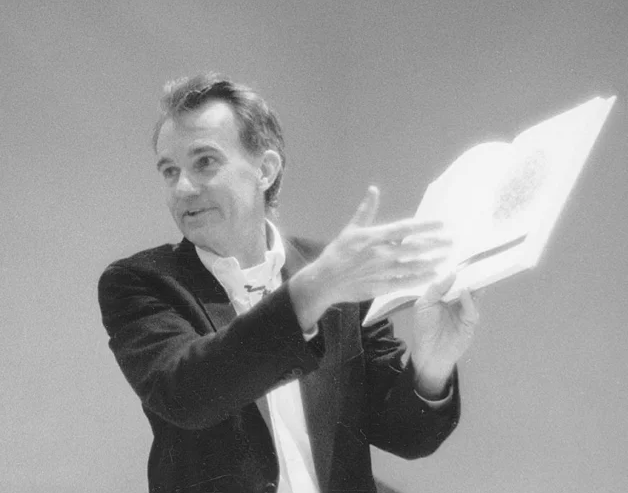
\includegraphics[width=\columnwidth]{edward_tufte.png}
        \caption{\scriptsize Edward Tufte(1942-),美国统计学家,数据可视化理论的先驱者和领军人物,人称“数据
    达芬奇”}
      \end{figure}
    \end{column}

    \begin{column}{.6\textwidth}
  \begin{ornamentblock}
    {The commonality between science and art is in trying to see profoundly - to develop strategies of seeing and showing.\\
      \rightline{\textemdash Edward Tufte}}
  \end{ornamentblock}
    \end{column}
  \end{columns}
\end{frame}

\begin{frame}{图形的价值}
  \begin{columns}
    \begin{column}{.3\textwidth}
      \begin{figure}
        \centering 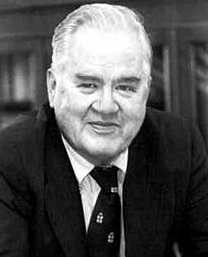
\includegraphics[width=\columnwidth]{john_tukey.png}
        \caption{\scriptsize John Tukey(1915-2000),美国著名数学家,箱线图发明者}
      \end{figure}
    \end{column}

    \begin{column}{.7\textwidth}
  \begin{ornamentblock}
    {The greatest value of a picture is when it forces us to notice what we never expected to see.\\
      \rightline{\textemdash John Tukey}}
  \end{ornamentblock}
    \end{column}
  \end{columns}
\end{frame}


%%%%%%%%%%%%%%%%
 \subsection{线图}

\begin{frame}[c]{线图(line chart)}{}
\begin{overlayarea}  {\textwidth}{\textheight}
  \only<1>{
    \begin{figure}
      \centering
      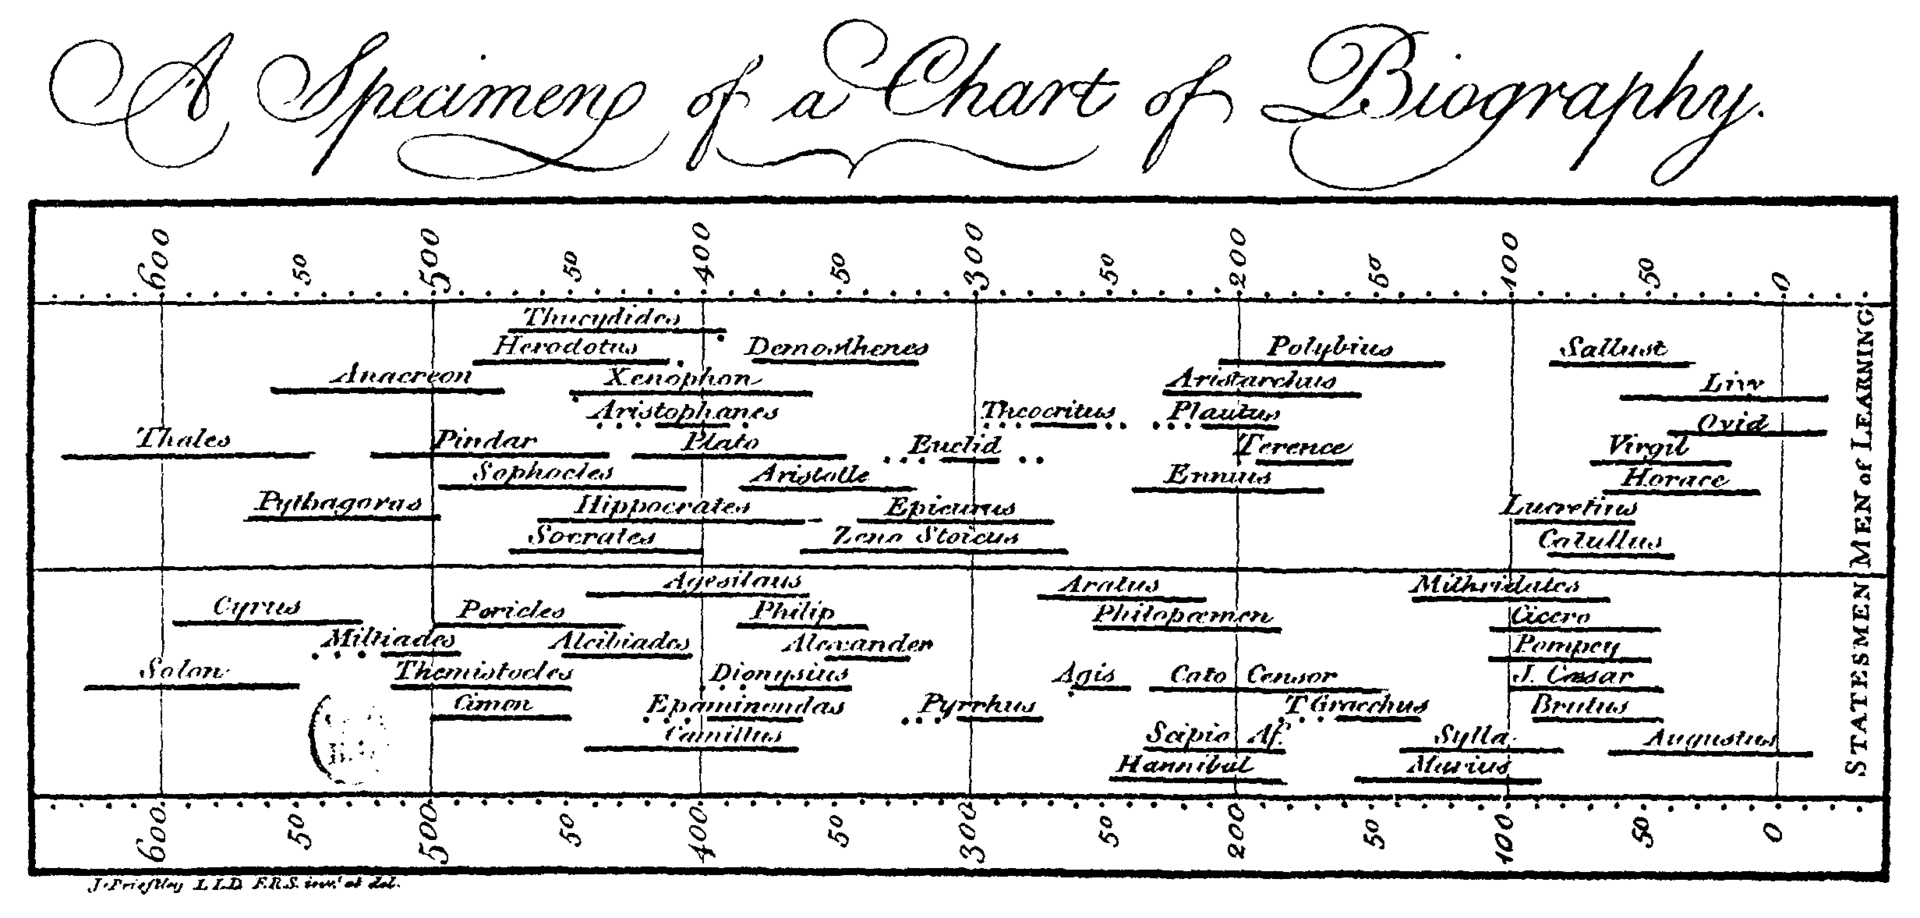
\includegraphics[width=\textwidth]{Priestley_Chart.png}
      \caption{英国化学家Joseph Priestley于1765年绘制的时间线图
        是\emphText{历史上最早的统计图形},这幅图展示了多个历史人物在历
        史长河中的跨度}
    \end{figure}} \only<2>{
    \begin{figure}
      \centering
      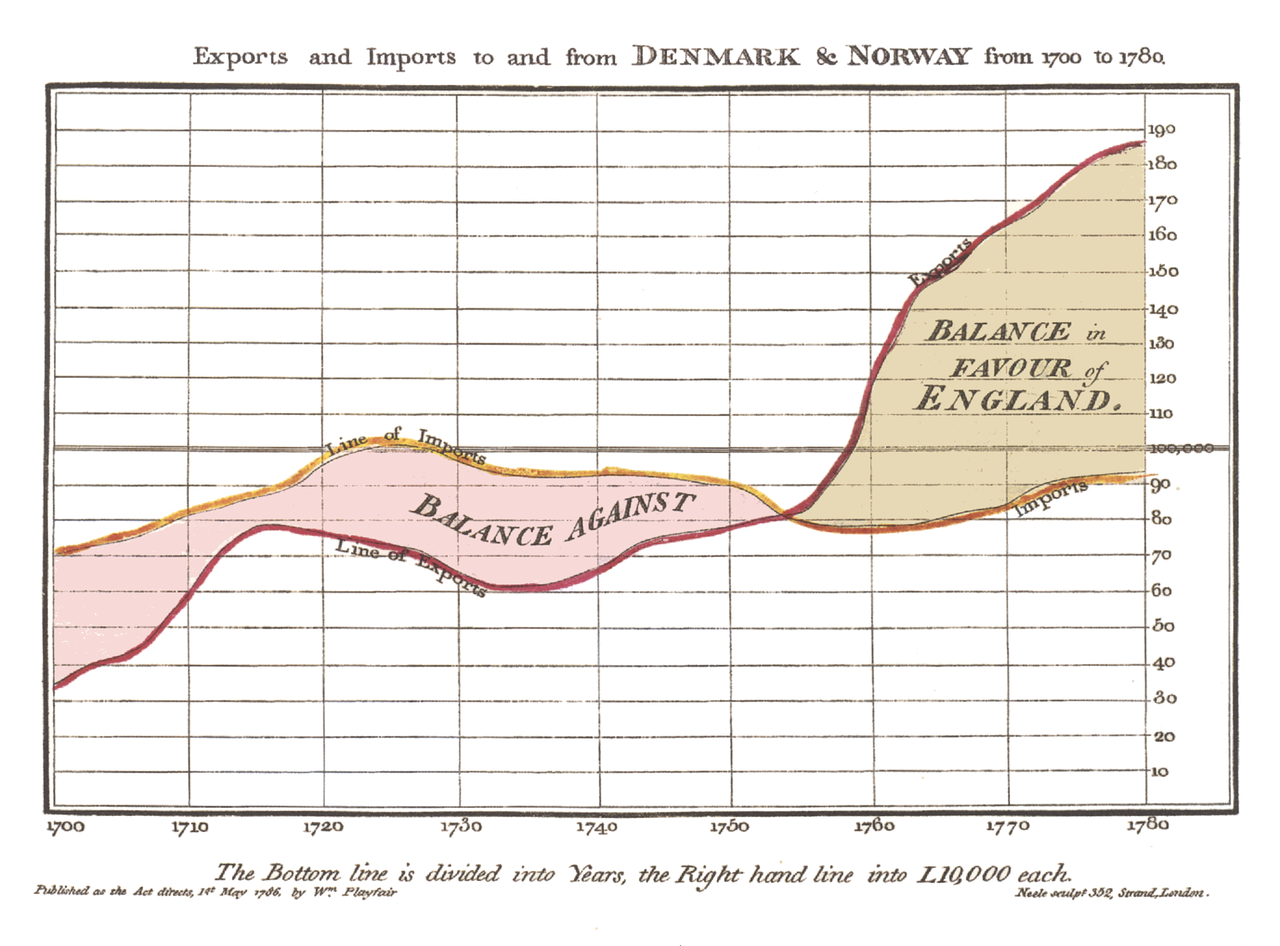
\includegraphics[width=0.75\textwidth]{Playfair_TimeSeries.png}
      \caption{苏格兰工程师和政治经济学家William Playfair于1786年在《Commercial and Political Atlas》
        一书中绘制的线图,这幅图展示了1700年至1780年间英格兰的进出口时序数据。\emphText{Playfair是历史上第一个系统使用统计图形的人,被称为“统计图形奠基人”}}
    \end{figure}}
\end{overlayarea}
\end{frame}

\subsection{柱状图}
\begin{frame}[c]{柱状图(bar chart)}{}
  \begin{figure}
    \centering
    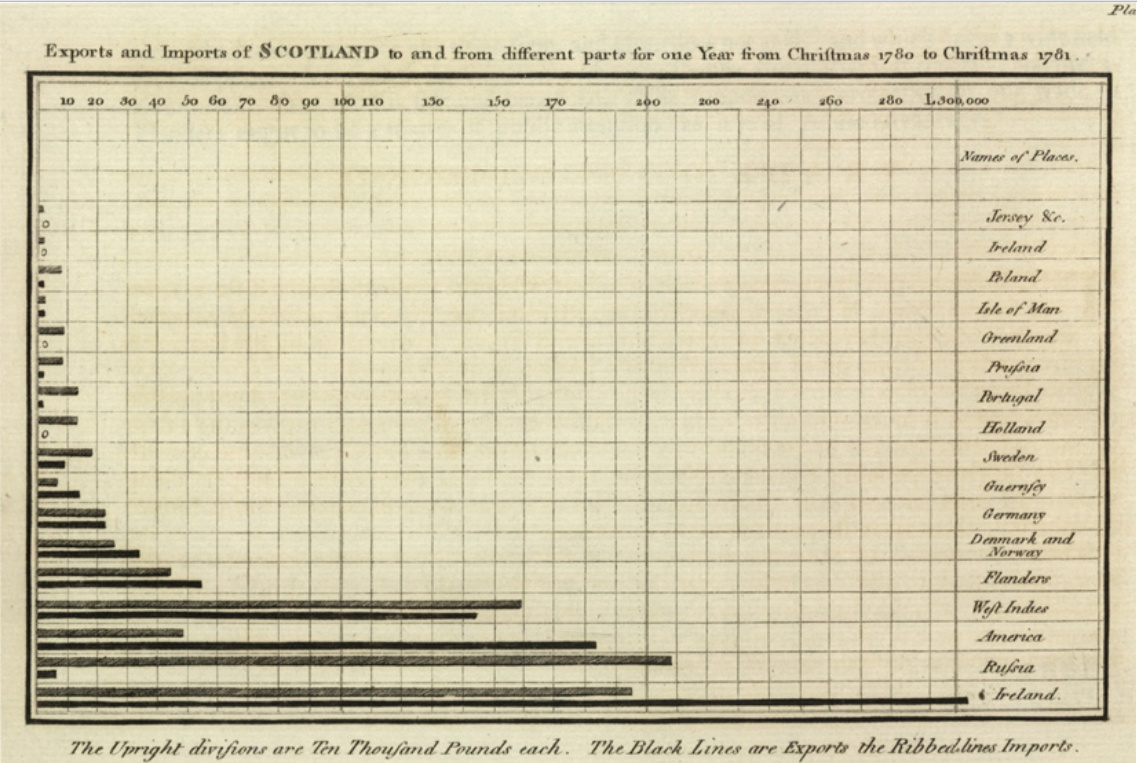
\includegraphics[width=0.8\textwidth]{Playfair_barchart.jpg}
    \caption{受到Priestley时间线图的影响,Playfair于1786年同样在
      《Commercial and Political Atlas》这本书中绘制了\emphText{历史上
        最早的柱状图},这幅图展示了不同国家的进出口数据}
  \end{figure}
\end{frame}

\subsection{饼图}

\begin{frame}[c]{饼图(pie chart)}{}
  \begin{figure}
    \begin{columns}
      \begin{column}{.6\textwidth}
        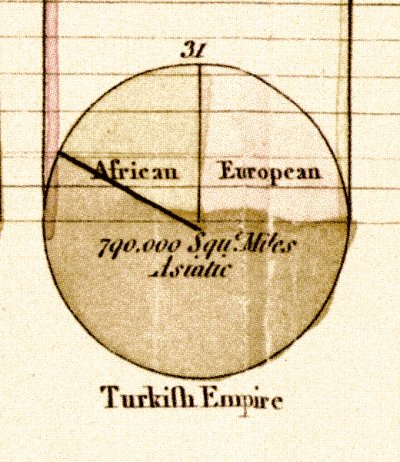
\includegraphics[width=\textwidth]{Playfair_piechart.jpg}
      \end{column}

    \begin{column}{.35\textwidth}
      \centering
      \caption{Playfair于1801年在《Statistical Breviary》这本书中绘制
        了\emphText{历史上第一幅饼图},这幅图展示了土耳其帝国在三大洲的
        国土面积分布情况}
    \end{column}
  \end{columns}
\end{figure}
\end{frame}

\subsection{主题统计地图}
\subsubsection{法国文盲率分布图}
\begin{frame}{\subsecname}{\subsubsecname}

  \begin{figure}
    \begin{columns}
      \begin{column}{.6\textwidth}
        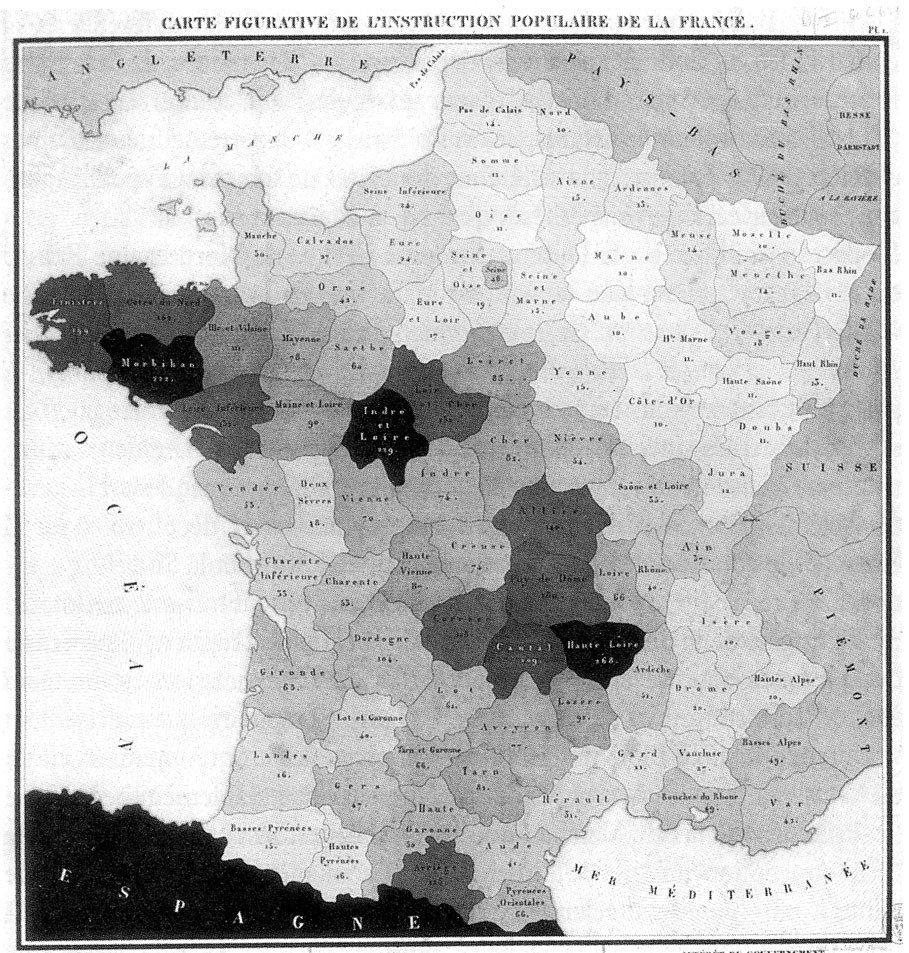
\includegraphics[width=\columnwidth]{法国文盲分布图.jpg}
      \end{column}

      \begin{column}{.35\textwidth}
        \centering
        \caption{法国文盲分布图(Charles Dupin, 1826). \\
          Charles Dupin是法国数学家,工程师,经济学家以及政客。1826年,
          他首次运用区域灰度地图的表现手段来展示法国当时的文盲率分布情
          况,\emphText{这是第一张现代形式的主题统计地图}}
      \end{column}
    \end{columns}
  \end{figure}
\end{frame}

\subsubsection{拿破仑东征图}
\begin{frame}{\subsecname}{\subsubsecname}
  \begin{figure}
    \centering 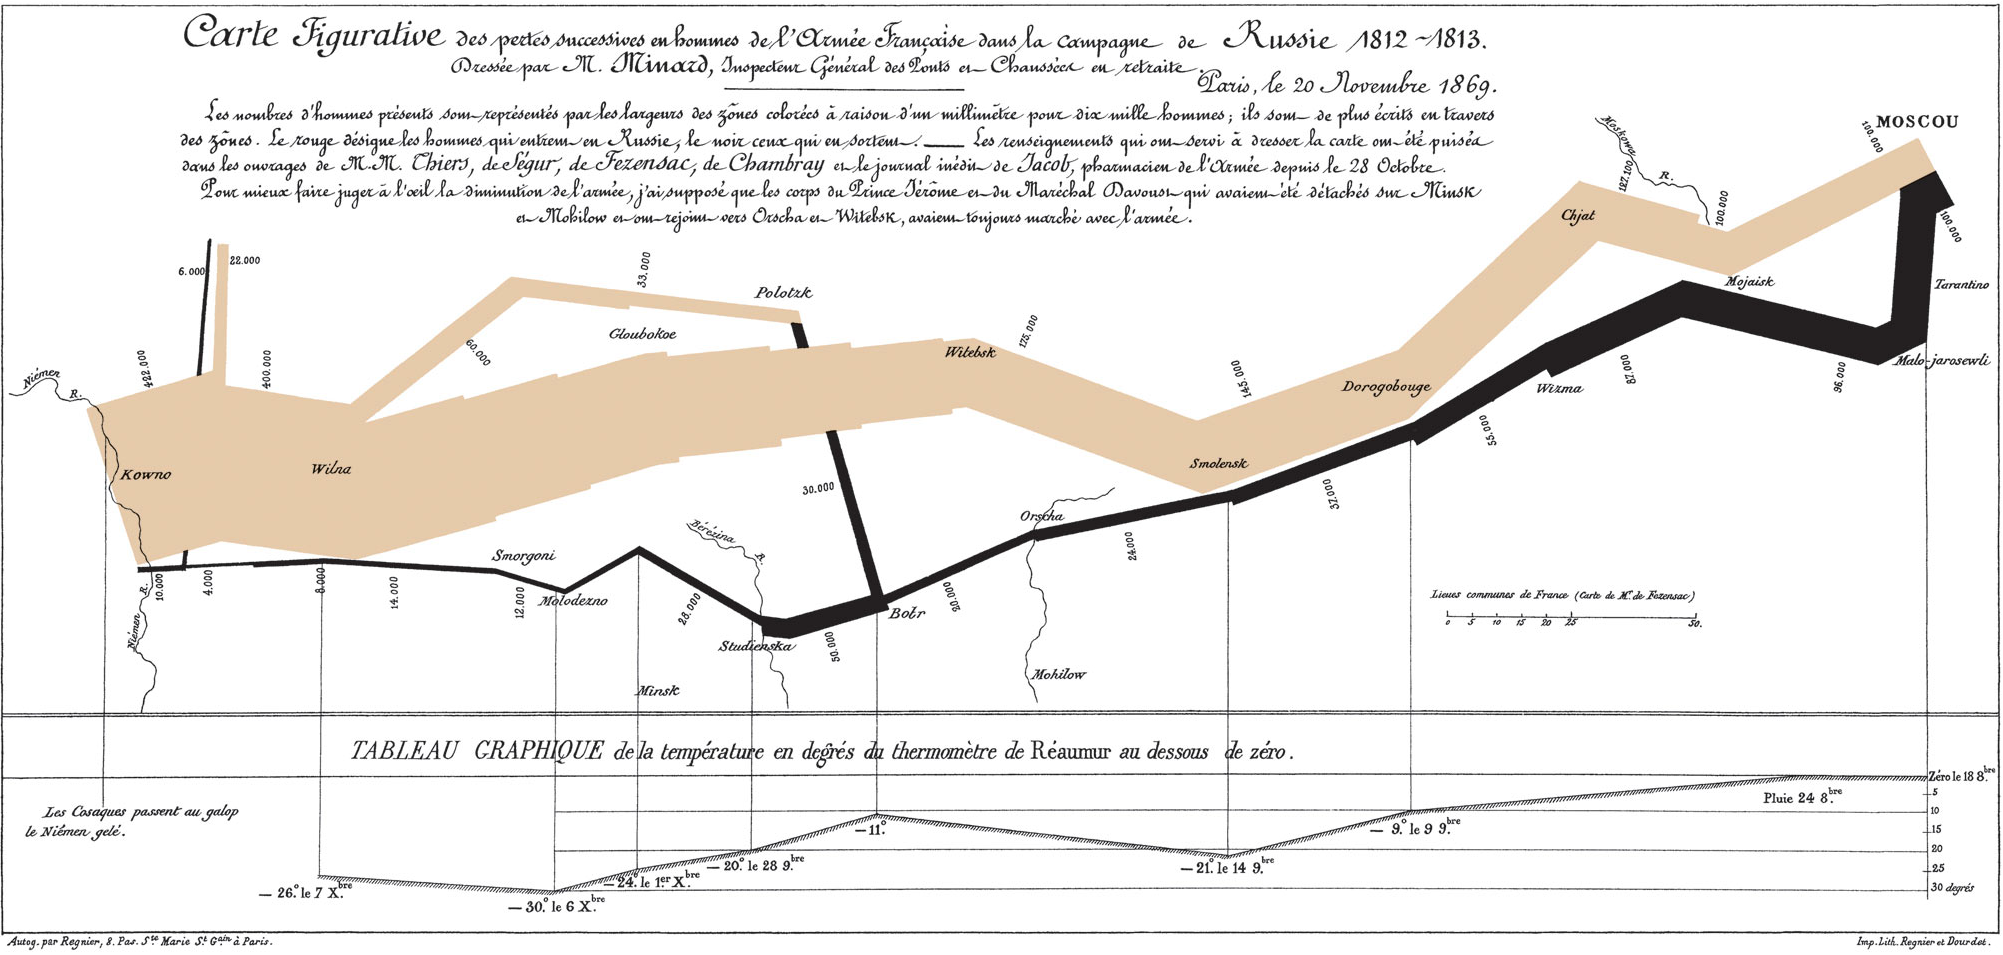
\includegraphics[width=0.8\columnwidth]{Minard.png}
    \caption{拿破仑东征图(Charles Joseph Minard, 1861). \\
      1861年,由法国工程师 Charles Joseph Minard 绘制,描述了1812年拿破
      仑东征俄罗斯的失败战役。图中同时包含了多个信息,粗细代表军队规模,
      配合日期标明了军队位置经纬度,棕色进军黑色撤退,下方折线展现气温,
      另标注了战斗的关键事件等信息。\\这幅图形在统计图形界内享有至高无上的
      地位,经常被一些统计、设计课程当作教学案例,被Edward
      Tufte誉为\emphText{“有史以来最好的统计图形”}}
  \end{figure}
  %\footnotetext[1]{Tufte是统计图形和信息可视化领域的领军人物,人称“数据达芬奇”}
\end{frame}

\subsubsection{汉尼拔远征图}
\begin{frame}{\subsecname}{\subsubsecname}
 \begin{figure}
   \centering 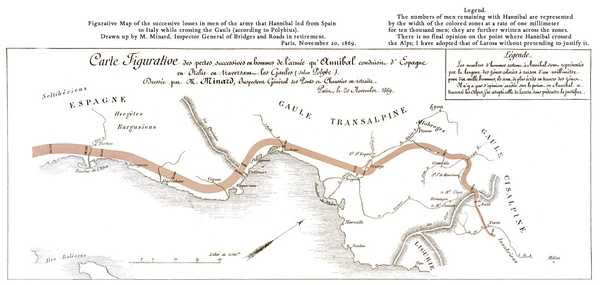
\includegraphics[width=\columnwidth]{汉尼拔远征图.jpg}
   \caption{汉尼拔远征图(Charles Joseph Minard, 1861)}
 \end{figure}
\end{frame}

\subsubsection{法国各地向巴黎输送牲畜产品的分布情况图}
\begin{frame}{\subsecname}{\subsubsecname}
  \begin{figure}
    \begin{columns}
      \begin{column}{.6\textwidth}
        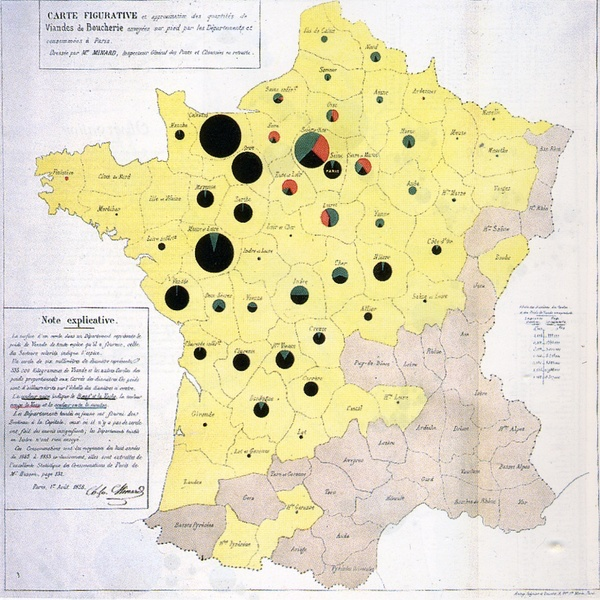
\includegraphics[width=\columnwidth]{法国各地向巴黎输送牲畜产品的分布情况图.jpg}
      \end{column}

      \begin{column}{.35\textwidth}
        \centering
        \caption{法国各地向巴黎输送牲畜产品的分布情况图(Charles Joseph Minard, 1858)\\
          此图的作者也是Joseph Minard,\emphText{经典之处在于首次将饼图融合到地图中}\\
          这位法国工程师,将一生大部分时间都贡献给了水坝,运河和桥梁的
          工程建造与教育事业,直到1851年退休,已近70岁高龄才正式开始研究数据信息图形可视化。在他最后的20年
          里,Minard在这个领域贡献了许多创新,共绘制了51幅各种形式的
          可视化图形,是那个可视化黄金时代当之无愧的大师,\emphText{被
            称为法国的“William Playfair”}}
      \end{column}
    \end{columns}
  \end{figure}
\end{frame}

\subsubsection{美国内战对欧洲棉花贸易的影响}
\begin{frame}{\subsecname}{\subsubsecname}
 \begin{figure}
   \centering 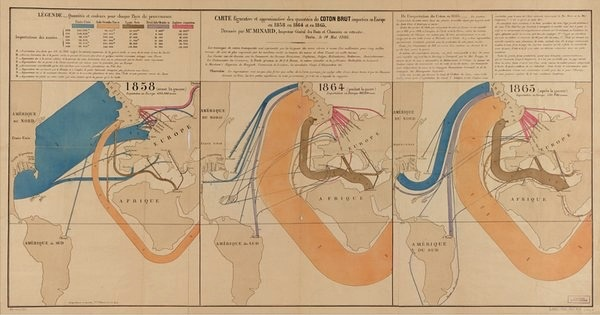
\includegraphics[width=\columnwidth]{美国内战对欧洲棉花贸易的影响.jpg}
   \caption{美国内战对欧洲棉花贸易的影响(Charles Joseph Minard, 1865)}
 \end{figure}
\end{frame}

\subsubsection{法国红酒出口情况}
\begin{frame}{\subsecname}{\subsubsecname}
 \begin{figure}
   \centering 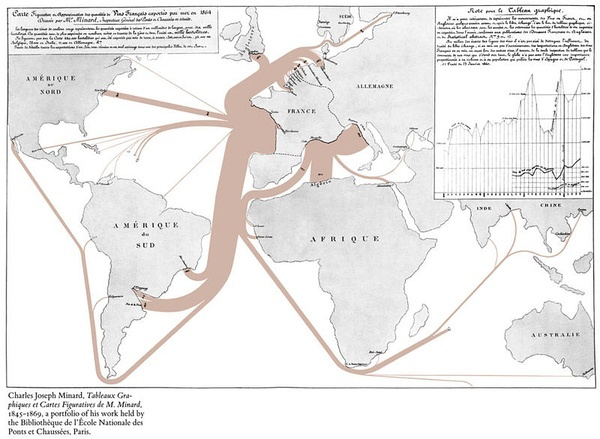
\includegraphics[width=0.8\columnwidth]{法国红酒出口情况.jpg}
   \caption{美国内战对欧洲棉花贸易的影响法国红酒出口情况(Charles
     Joseph Minard, 1864)}
 \end{figure}
\end{frame}

\subsubsection{地铁路线图}
\begin{frame}{\subsecname}{\subsubsecname}
  \begin{figure}\centering
    \subfloat[1908年版]
    {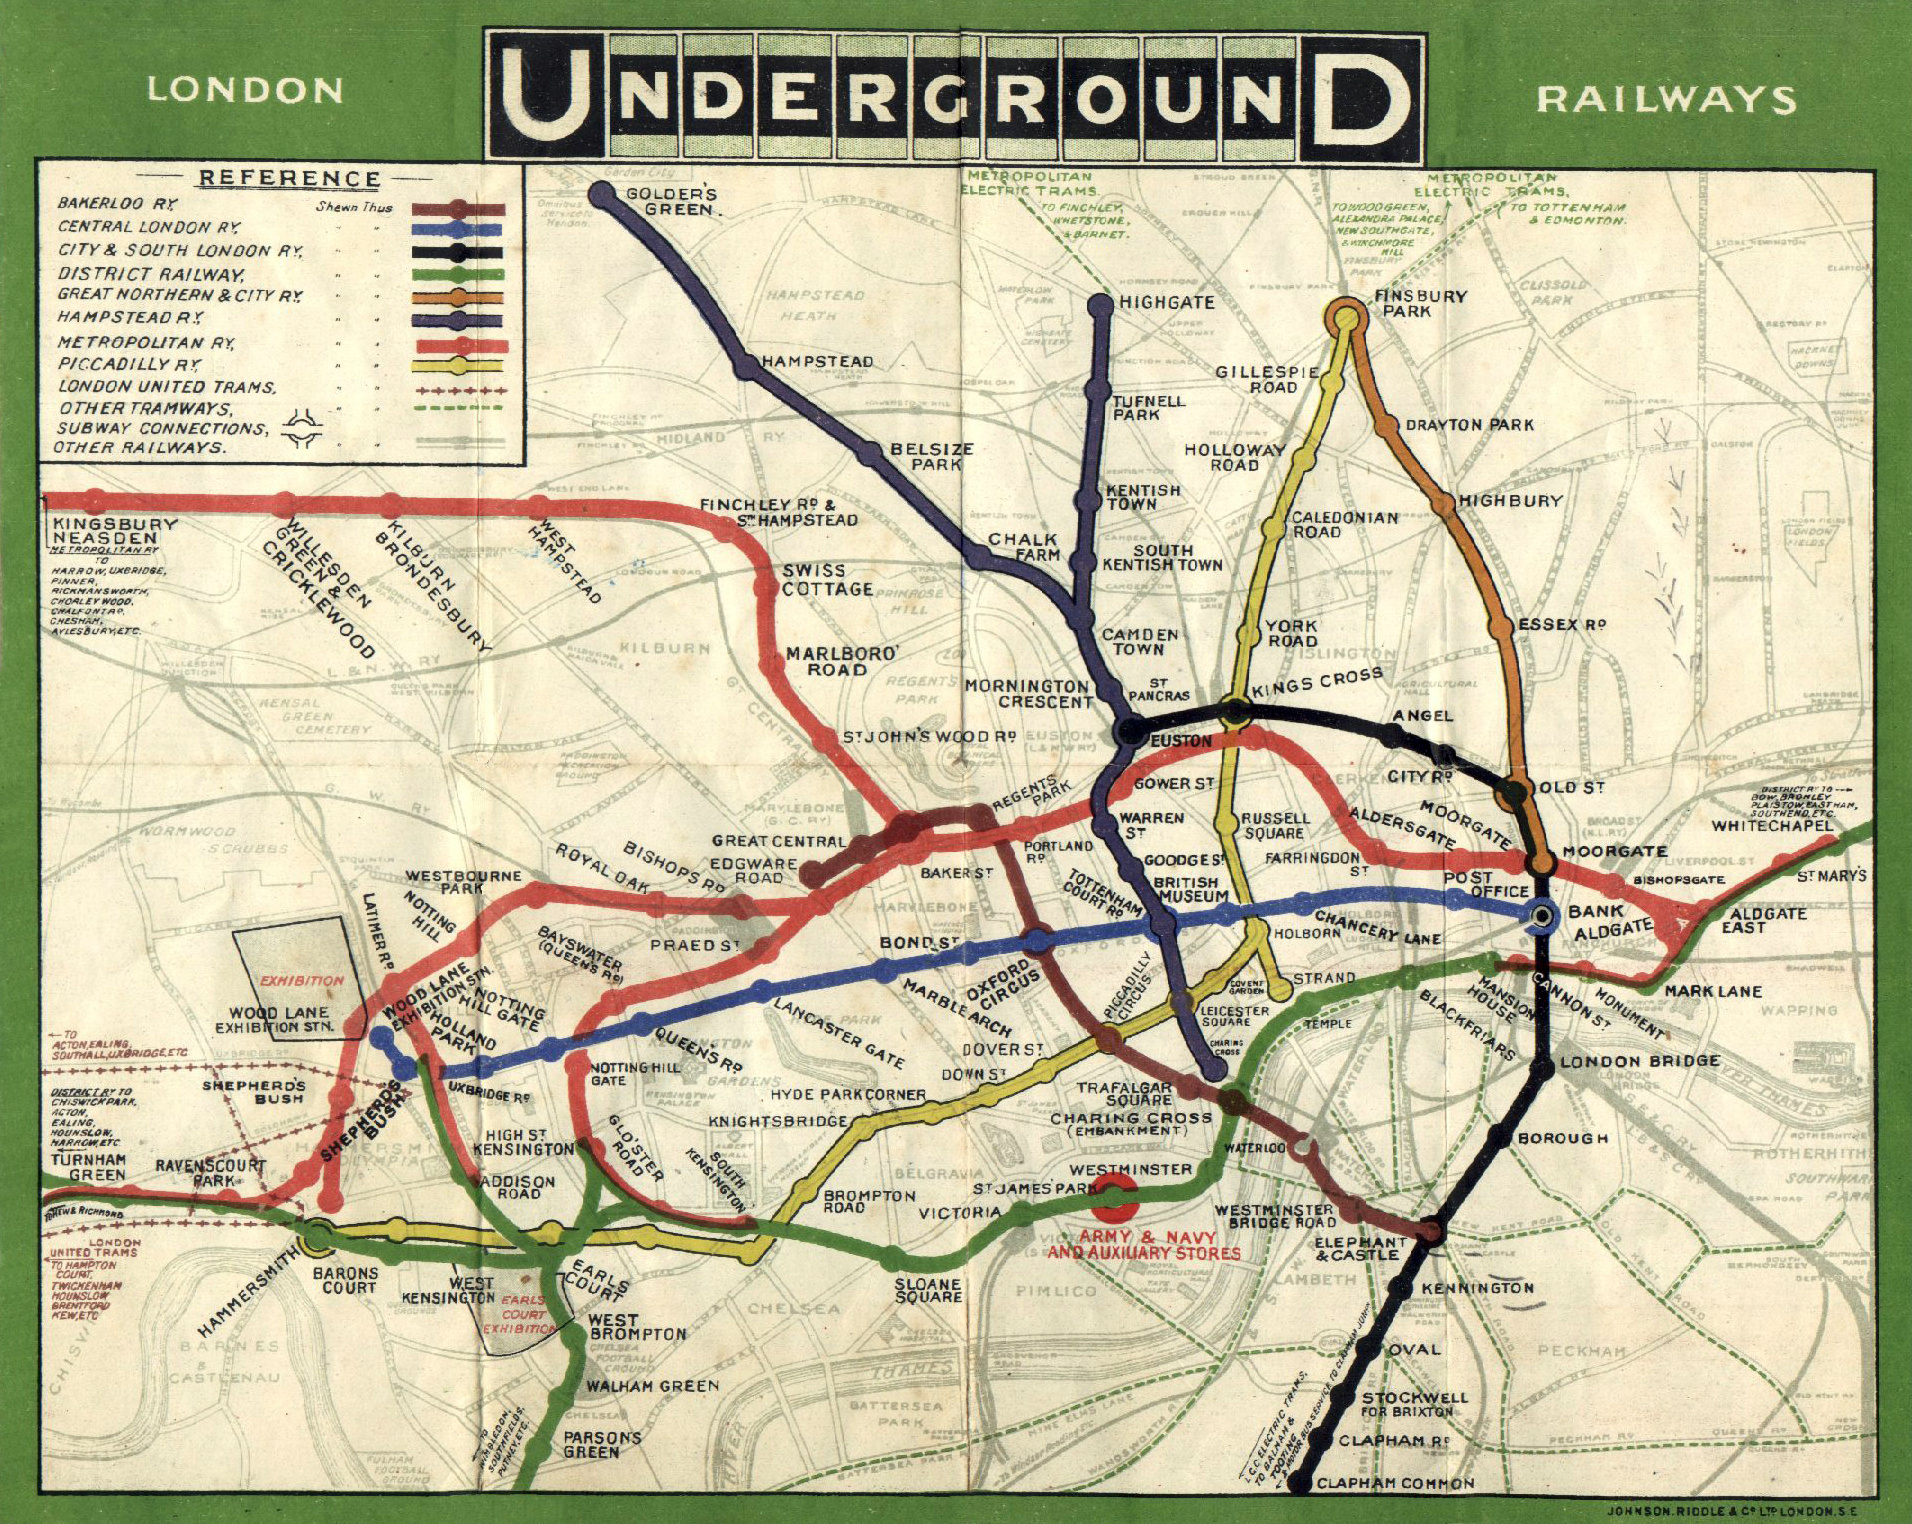
\includegraphics[height=0.4\textheight]{1908年伦敦地铁路线图.jpg}}\vspace{0.5pt} 
    \subfloat[1933年版]
    {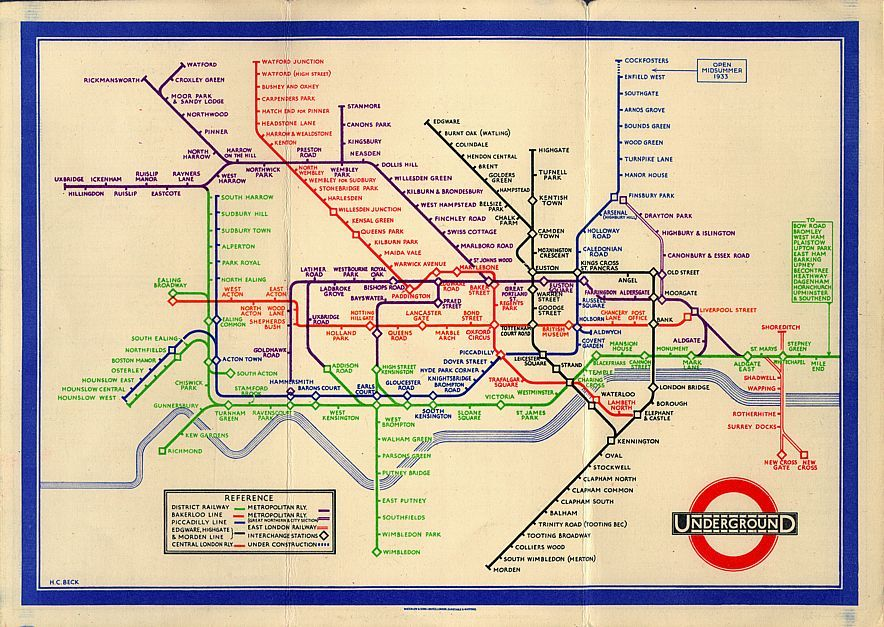
\includegraphics[height=0.4\textheight]{1931年贝克设计的伦敦地铁路线图.jpg}}
    \caption{道路网络形状更新在最早的地图中都是按照实地比例进行绘制的,
      比如左图的1908版伦敦地铁线路图。1931年,英国技术制图员Harry
      Beck在替伦敦地铁的讯号室绘制电路图时受到启发,设计出了经典
      的1933年版路线图(右图)}
  \end{figure} 
\end{frame}

\subsubsection{变形地图}
\begin{frame}{\subsecname}{变形地图(cartogram)}
  \begin{figure}\centering
    \subfloat[普通色块地图表达]
    {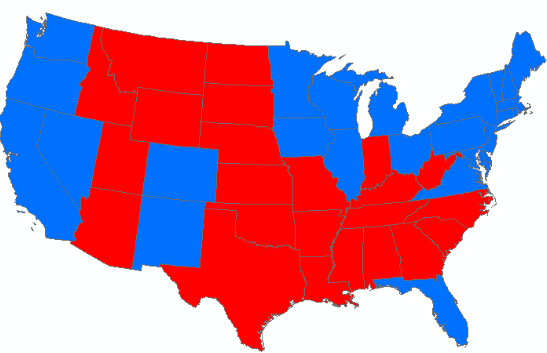
\includegraphics[width=0.45\columnwidth]{cartogram1.png}}\vspace{0.5pt}
    \subfloat[变形地图表达]
    {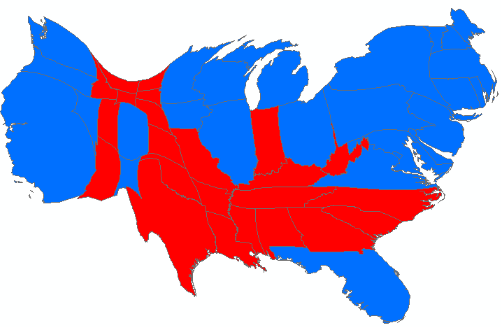
\includegraphics[width=0.45\columnwidth]{cartogram2.png}}
    \caption{变形地图的历史可以追溯到1868年,\emphText{其作用是用夸张的地图变形来表达真实的数量关系}\\上面左图是2012年
      美国大选的结果,从普通色块图上看似乎是红色代表的罗姆尼获胜,但其实获胜的是蓝色代表的奥巴马;右图是根据选票
      数量进行变形处理后的地图,可以很清楚看到蓝色多于红色,这才是真实数量的正确表达!}
  \end{figure}
\end{frame}

\subsection{统计图形的应用}
\subsubsection{南丁格尔玫瑰图}
\begin{frame}{\subsecname}{\subsubsecname}
 \begin{figure}
   \centering
   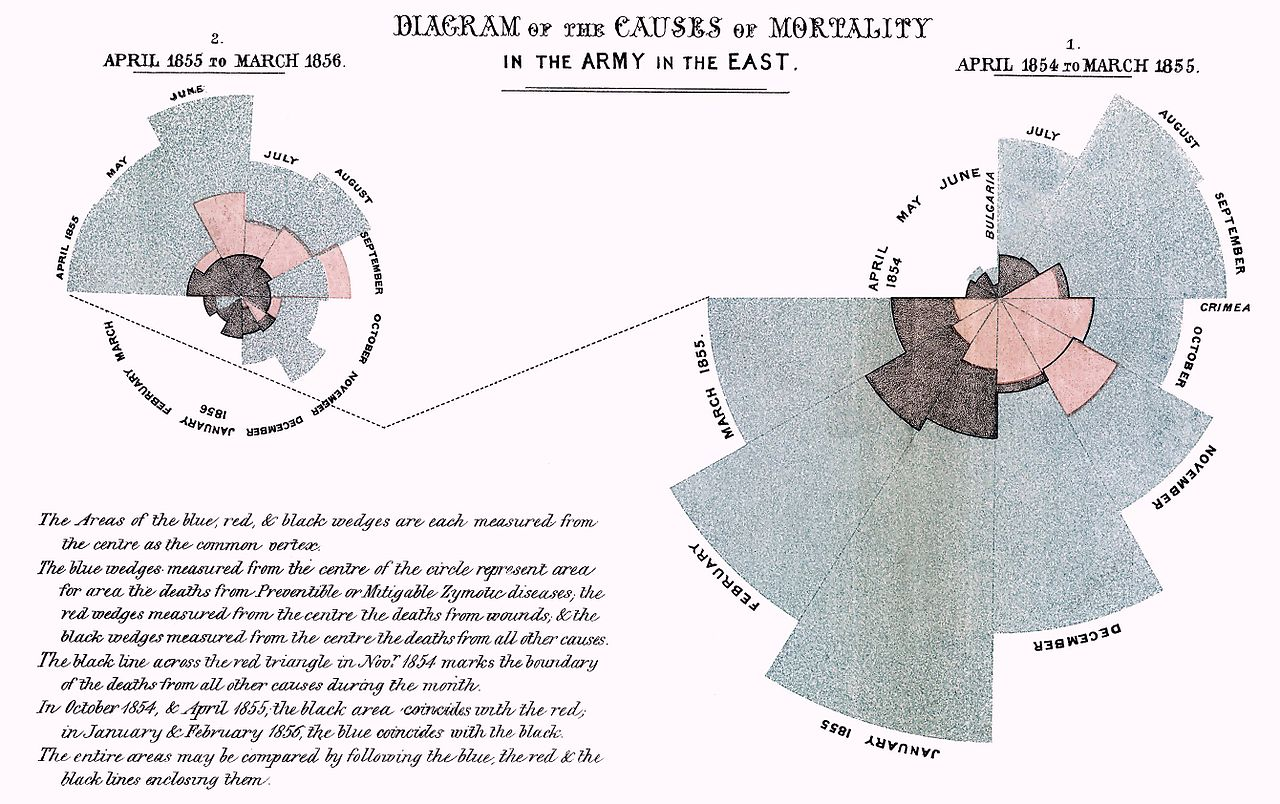
\includegraphics[width=0.8\columnwidth]{Nightingale_mortality.jpg}
   \caption{上图是南丁格尔玫瑰图。两幅图分别表示1854年和1855年军队的伤
     亡人数,
     一年12个月在极坐标上被分为12等分,每一个花瓣表示一个月;不同颜色表示死亡原因\\
     南丁格尔通过这幅图使英国政府意识到真正影响战争伤亡的并非战争本身,
     而是由于军队缺乏有效的医疗护理。由此,英国政府于1857年开设了专门的
     军医学校,培养专门的战地医护人员,\emphText{这就是统计图形在近代护
       理学最早的应用}}
 \end{figure}
\end{frame}

\subsubsection{霍乱传播之谜}
\begin{frame}{\subsecname}{\subsubsecname}
  \begin{figure}
    \begin{columns}
      \begin{column}{.6\textwidth}
        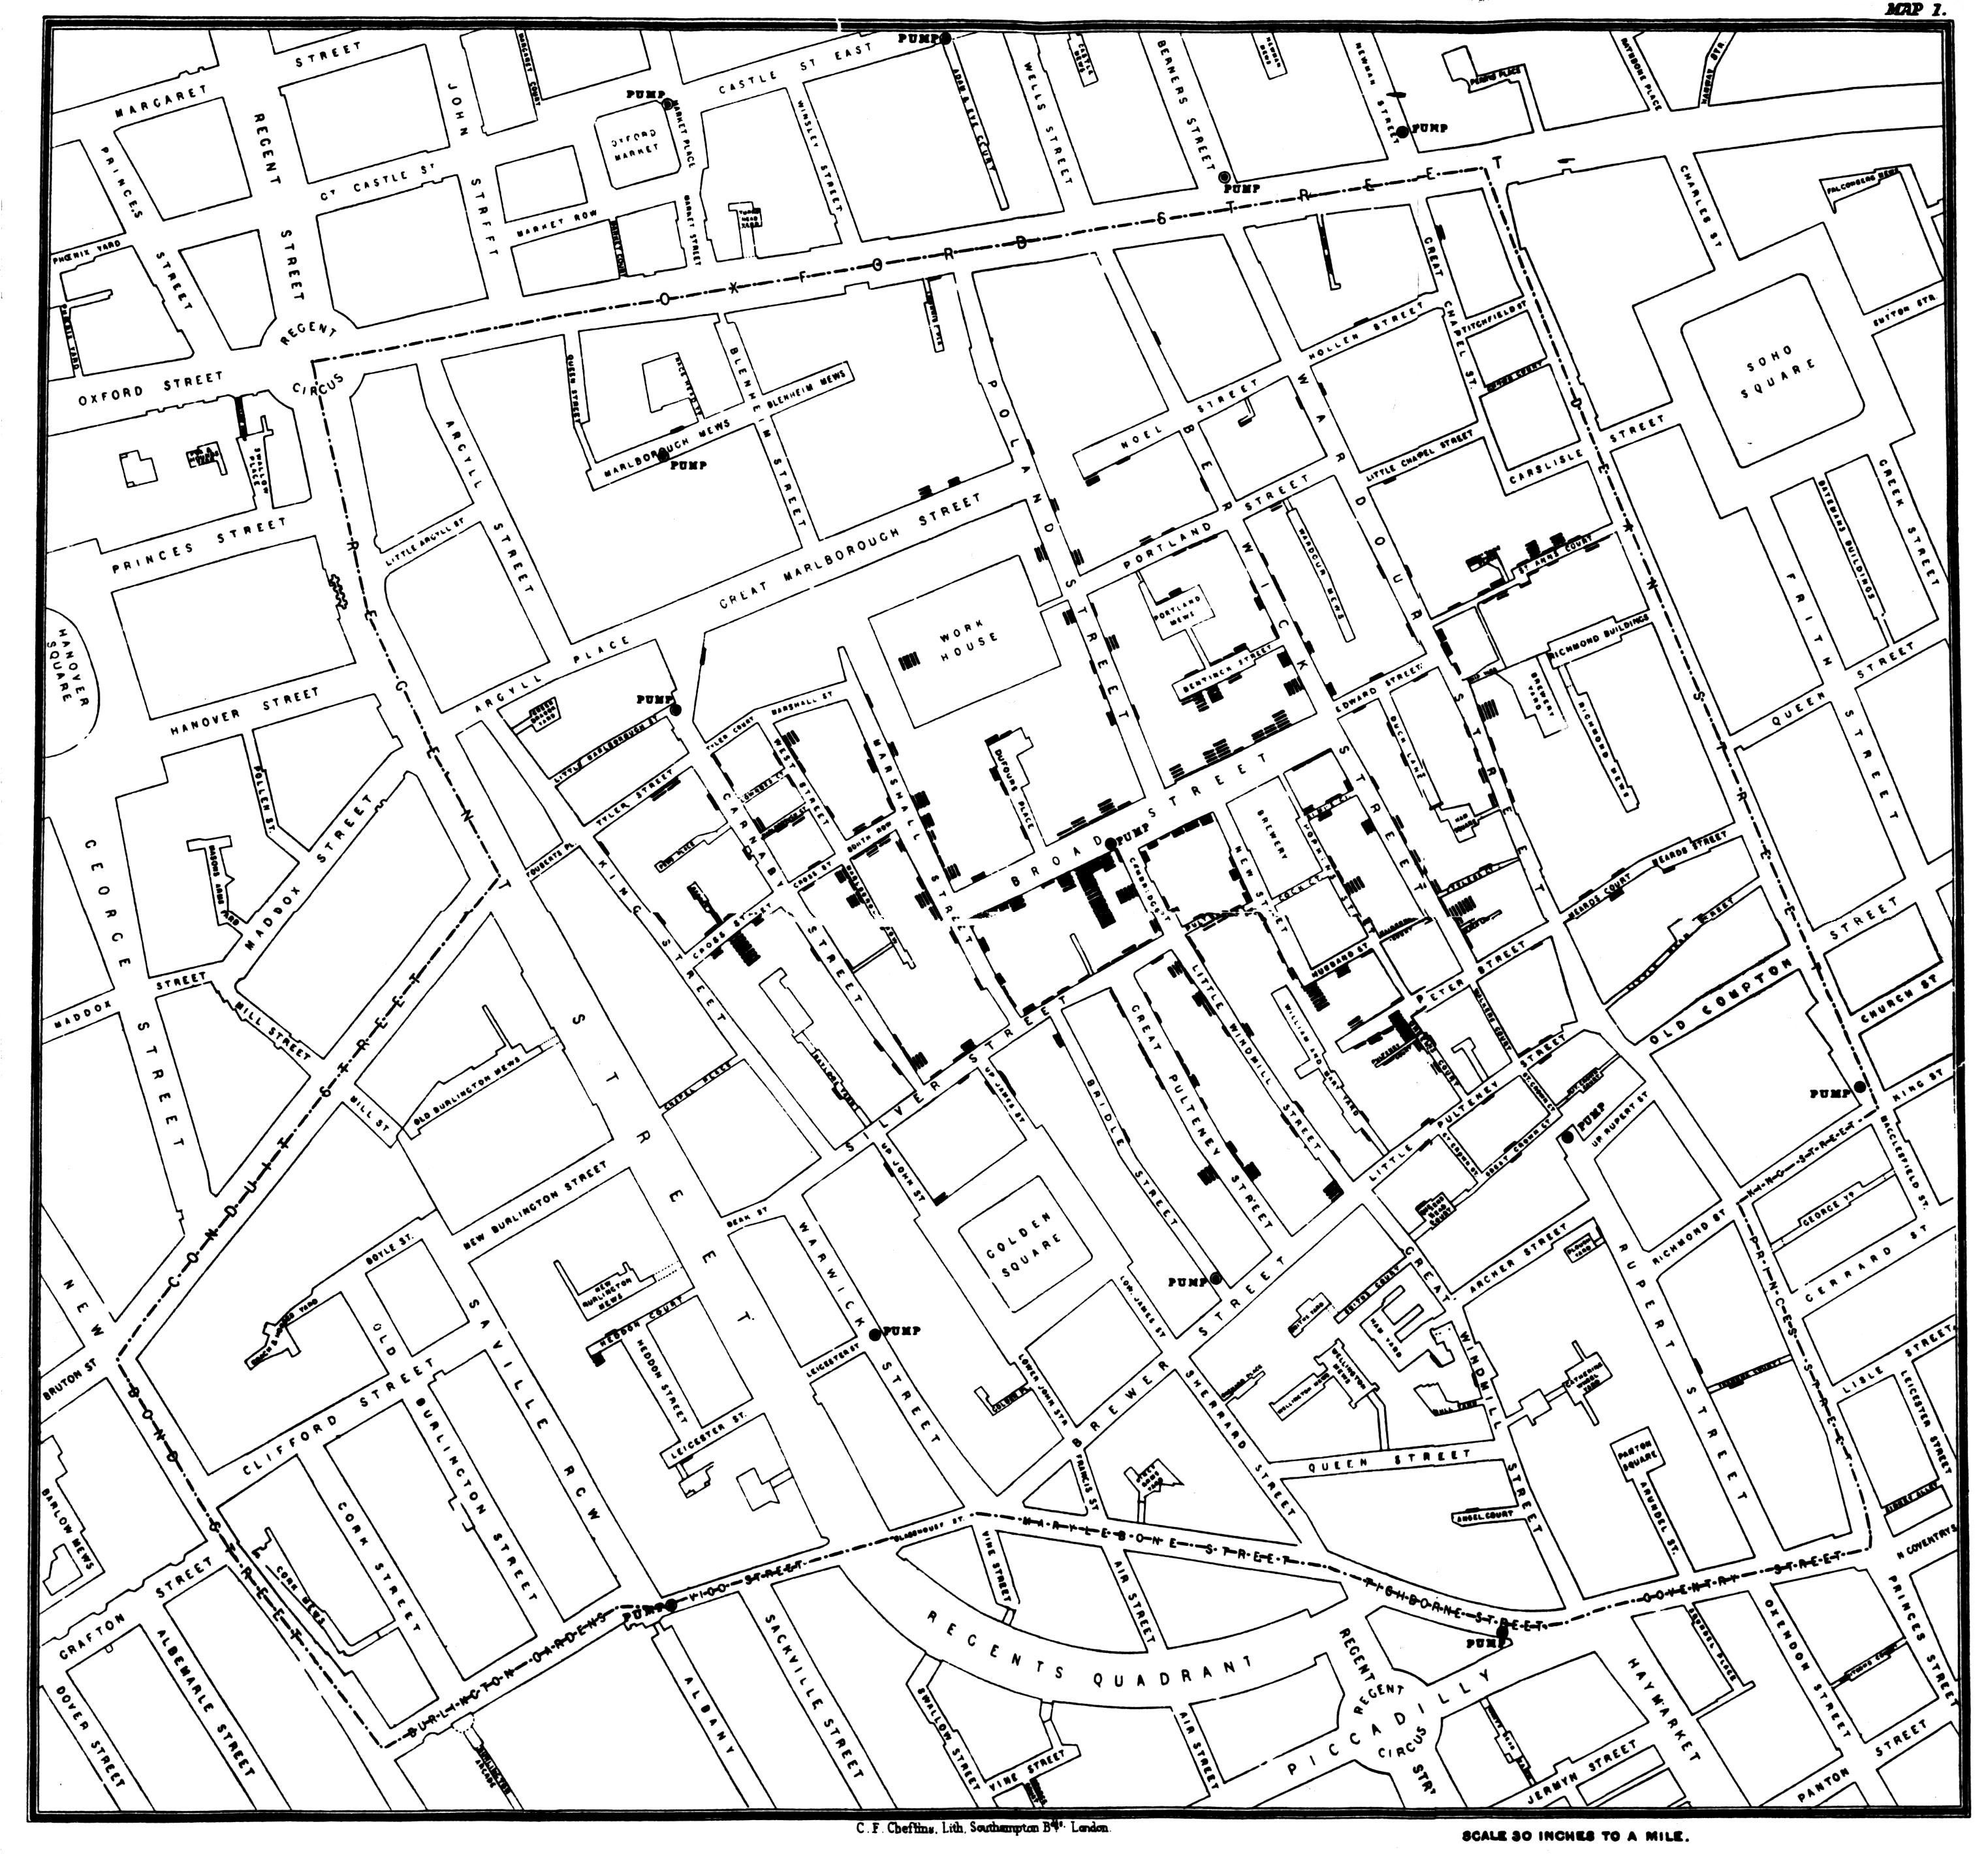
\includegraphics[width=\columnwidth]{Snow_cholera_map.jpg}
      \end{column}

      \begin{column}{.35\textwidth}
        \centering
        \caption{1854年英国Broad大街大规模爆发霍乱,流行病学家John
          Snow对此次霍乱进行了大量调研分析,并且发表了霍乱传播理论的论
          文,左图是其论文的主要依据:图中心东西
          方向的街道是Broad大街,黑点表示死亡地点\\
          这幅图形象揭示了一个重要现象,就是死亡地点都在街道中部一处水源
          (水井)周围,而市内其它水源周围极少发现死者,通过进一步调查他
          发现这些死者都饮用过这里的井水,从而发现了霍乱传播的源头是水
          井的把手,\emphText{这就是统计图形在公共卫生领域最早的应用}}
      \end{column}
    \end{columns}
  \end{figure}
\end{frame}

\begin{frame}{\subsecname}{\subsubsecname}
  \begin{figure}
    \begin{columns}
      \begin{column}{.6\textwidth}
        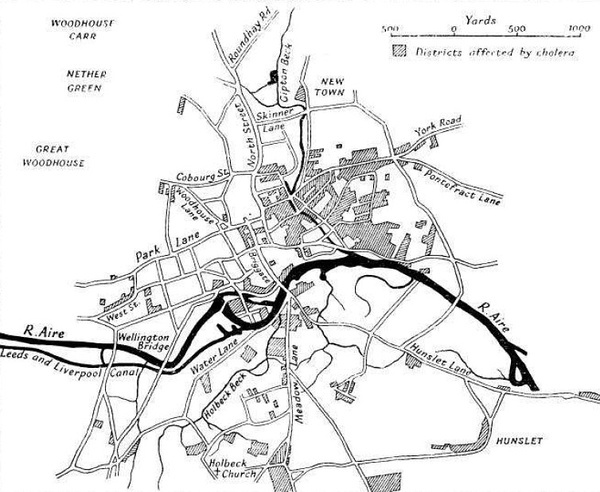
\includegraphics[width=\columnwidth]{Robert_Baker.jpg}
      \end{column}

      \begin{column}{.35\textwidth}
        \centering
        \caption{其实,在John Snow之前,有个叫Robert Baker的医生也研究
          了这个区域的霍乱问题,而且在1833年就绘制了左边这
          张霍乱的分布图。\\
          虽然Baker在这幅图中揭示了疾病和居住环境的联系:缺乏清洁用水和
          排水系统的居民点是疾病的高发区,\emphText{但是并没有显示发病
            率}。关于疾病起因的认知,他尽管方向正确但是并不完备,最终与
          伟大
          的发现擦肩而过\\
          \emphText{因此,只有充分完备的统计图形才能够真正应用于实践,
            这是一个漫长的科学过程}}
      \end{column}
    \end{columns}
  \end{figure}
\end{frame}

\subsubsection{切尔诺夫脸谱图}
\begin{frame}{\subsecname}{切尔诺夫脸谱图(Chernoff Faces)}
  \begin{figure}
    \begin{columns}
      \begin{column}{.6\textwidth}
        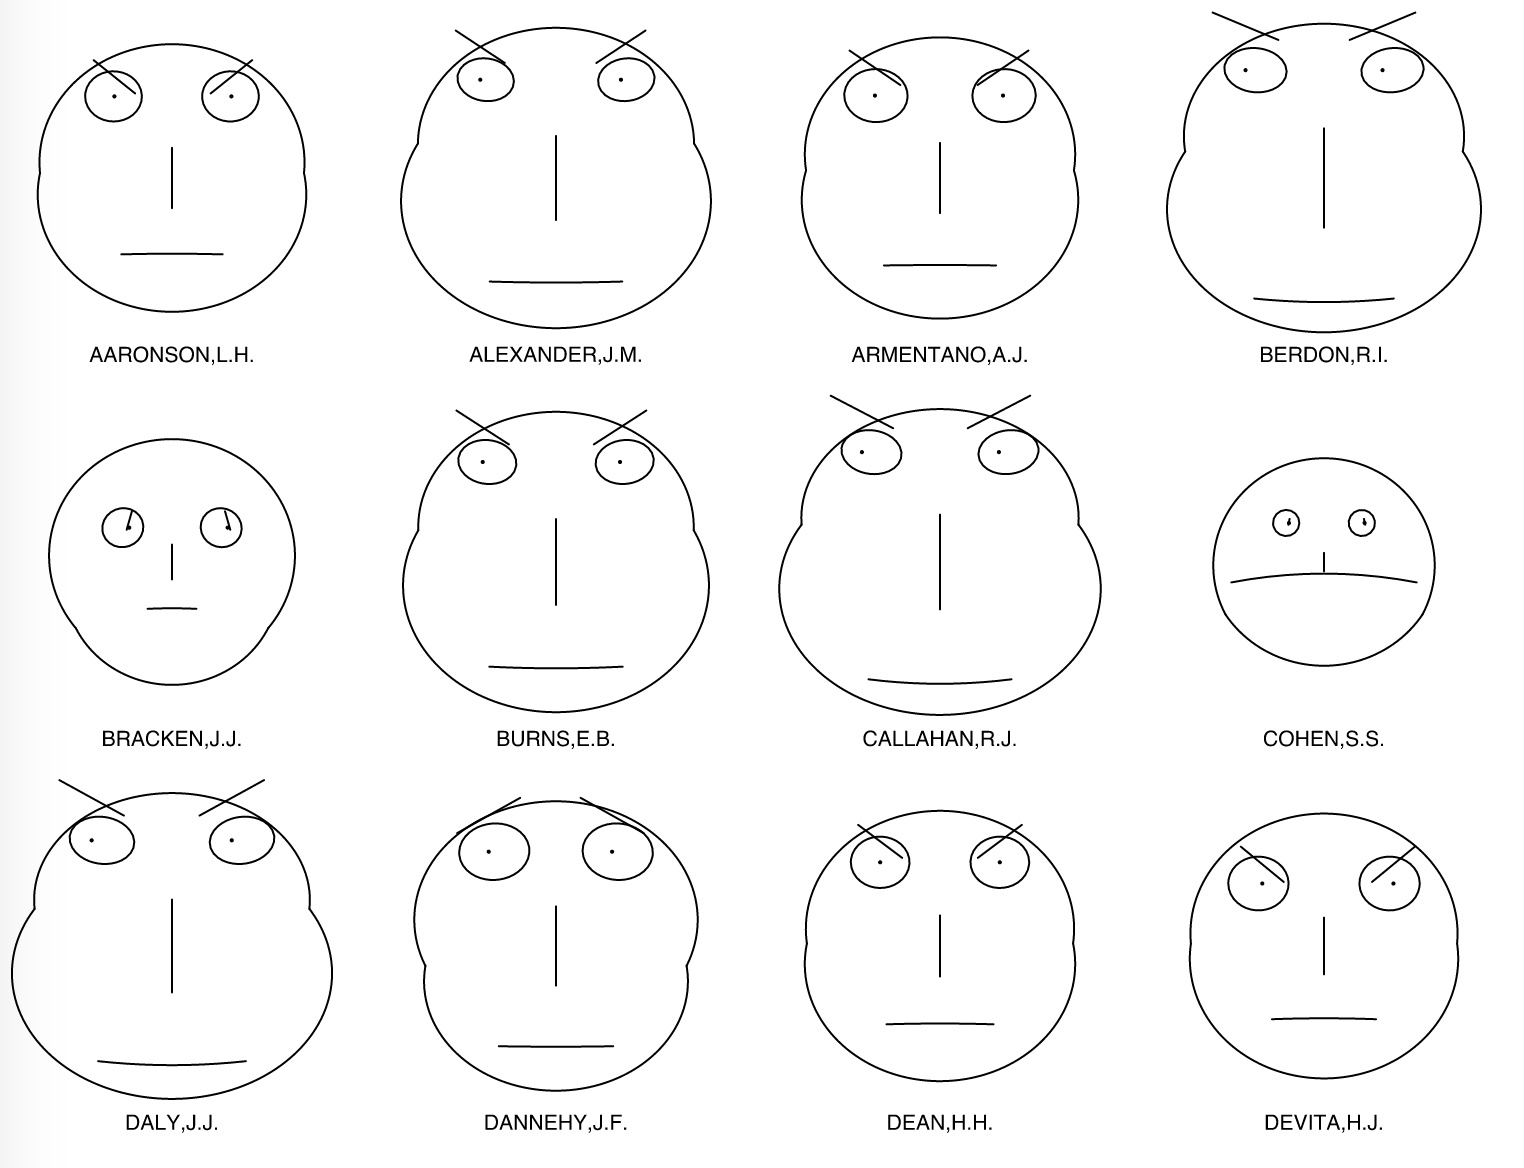
\includegraphics[width=\columnwidth]{切尔诺夫脸谱图.jpg}
      \end{column}

      \begin{column}{.35\textwidth}
        \centering
        \caption{切尔诺夫脸谱图(Herman Chernoff, 1973)\\
          这张很喜感的脸谱图其实是一种统计图,叫切尔诺夫脸谱图,是统计
          学家Herman Chernoff于1973年发明的,其基本思想是把多维数据的特
          征映射到卡通人脸中。由于人类非常善于识别脸部特征,脸谱化使得
          多维度数据容易被分析人员消化理解,有助于数据的规律和不规律性
          的可视化。\emphText{目前这种方法已被广泛应用于多地域经济战略
            指标数据分析,空间数据可视化等领域}}
      \end{column}
    \end{columns}
  \end{figure}
\end{frame}

%
%%% Local Variables:
%%% mode: latex
%%% TeX-master: "section02.tex"
%%% End:
%%%%%%%%%%%%%%%%%%%%%%%%%%%%%%%%%%%%%%%%%%%%%%%%%%%%%%%%%%%%
\section{统计绘图工具}
%%%%%%%%%%%%%%%%%%%%%%%%%%%%%%%%%%%%%%%%%%%%%%%%%%%%%%%%%%%%
\subsection{何为利器}
\begin{frame}{\subsecname}{}

  \begin{columns}
    \begin{column}{.5\textwidth}
      \begin{figure}
        \centering 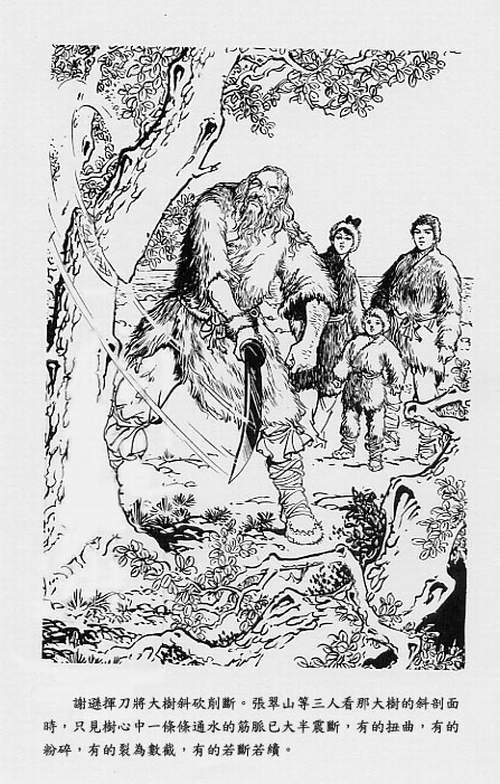
\includegraphics[width=\columnwidth]{屠龙宝刀.jpg}
      \end{figure}
    \end{column}

    \begin{column}{.5\textwidth}
      \begin{ornamentblock}
        \centering
        {君子性非异也,善假于物也\\ %工欲善其事,必先利其器《论语·卫灵公》
          \rightline{\textemdash 《荀子·劝学》}}
      \end{ornamentblock}
    \end{column}
  \end{columns}

\end{frame}

\begin{frame}[c]{\subsecname}
  
  \begin{columns}
    \begin{column}{.5\textwidth}
      \begin{figure}
        \centering 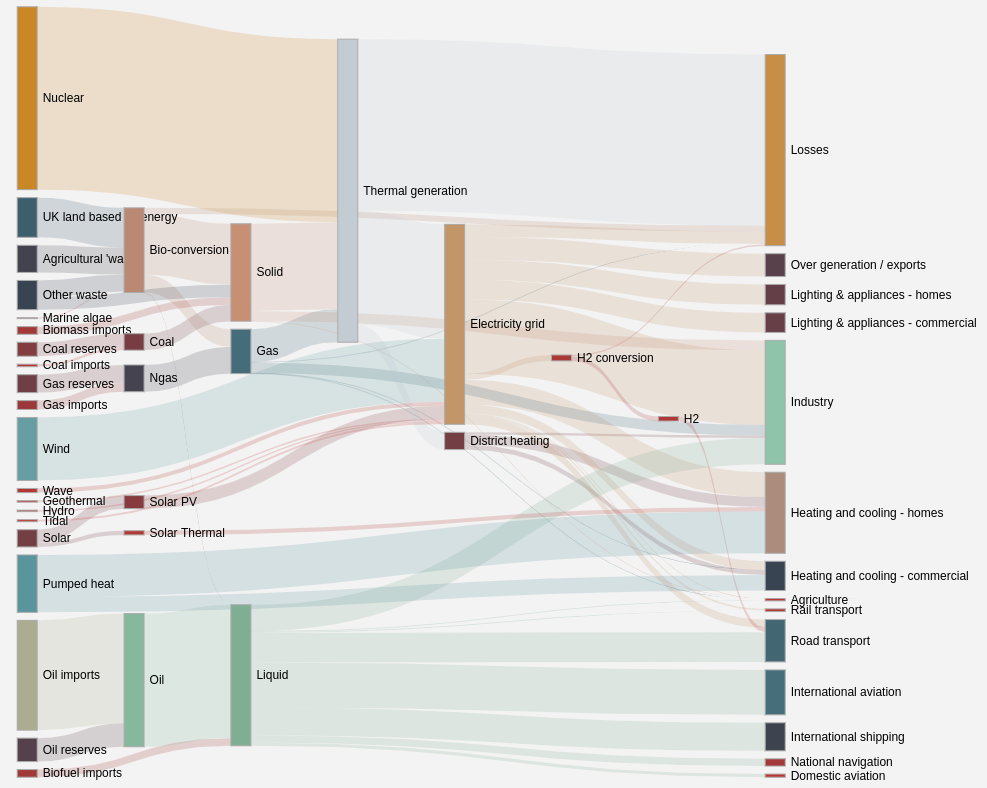
\includegraphics[width=\columnwidth]{sankey.png}
        \caption{看上去复杂但是直观的桑基图(Sankey diagram)}
      \end{figure}
    \end{column}

    \begin{column}{.5\textwidth}
      \begin{block}{\small 直观与简单} \small
        \begin{itemize}
        \item[\HandRight] \emphText{统计量是统计图形最关键的构成因素},
        因此,优秀的统计图形背后必然隐藏着重要的统计量
        \item[\HandRight] 图形的首要作用是“直观”展示统计量信息,
        但是\emphText{能够直观理解的信息未必是“简单”的}
        \item[\HandRight] 使用合适的工具可以让信息的表达既“直观”又“简单” 
        \end{itemize}
      \end{block}
    \end{column}
  \end{columns}
    
\end{frame}

%\subsection{何为利器}
\begin{frame}[t]{\subsecname}
  \begin{itemize}
    \item 统计计算功能齐全
    \item 图形元素易于控制
    \item 统计图形种类丰富
  \end{itemize}

\begin{figure}[ht]
  \centering 
\includegraphics[width=0.8\textwidth]{stat_tools.png}
  \caption{常见的一些统计绘图工具}
\end{figure}
\end{frame}

\subsection{所见即所得工具}
\subsubsection{excel}
\begin{frame}[t]{\subsecname}{\subsubsecname}
\begin{itemize}
\item<1-> 微软公司开发的电子数据表软件,从1985年发布1.0版本
    至今已经30多年历史,是电子数据表类软件的工业标准
\item<2-> 优秀的人机实时交互设计,所见即所得
\item<3-> 能够完成简单的统计功能以及数据绘图,但并不是统计软件
\end{itemize}

\begin{overlayarea}{\textwidth}{\textheight} 
  \only<1>{
    \begin{figure}\centering
      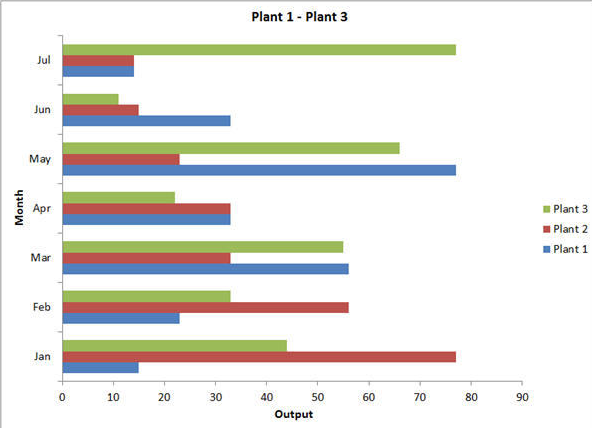
\includegraphics[width=0.65\columnwidth] {excel条形图.png}
      \caption{表示绝对数值大小的条形图}
    \end{figure}}

  \only<2>{
    \begin{figure}\centering
      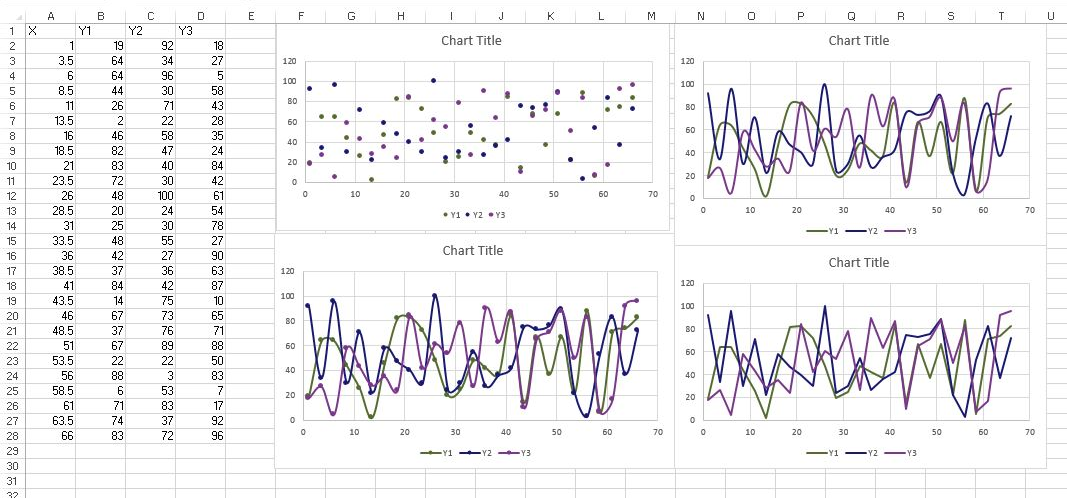
\includegraphics[width=\columnwidth] {excel折线图.png}
      \caption{表示绝对数值大小的折线图}
    \end{figure}}
  
  \only<3>{
    \begin{figure}[ht]
      \centering 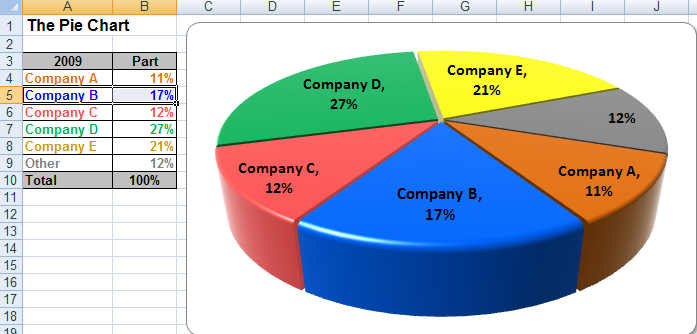
\includegraphics[width=\columnwidth]{excel饼图.png}
      \caption{表示比例大小的饼图}
    \end{figure}}

  \only<4>{
    \begin{figure}[ht]
      \centering 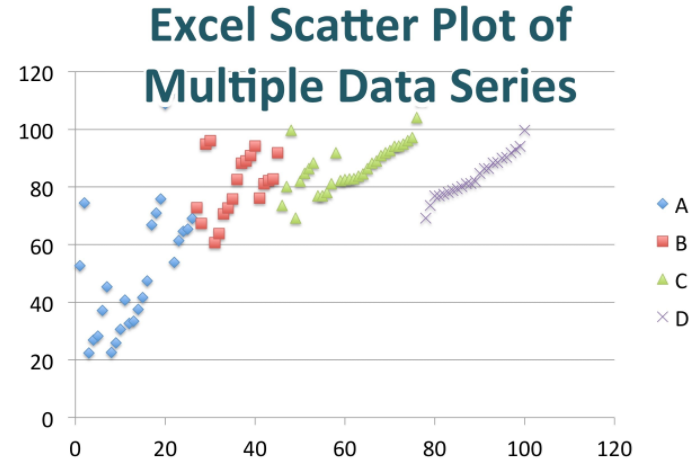
\includegraphics[width=0.7\columnwidth]{excel散点图.png}
      \caption{表示二维变量关系的散点图}
    \end{figure}}
   
  \only<5->{
    \begin{alertblock}{excel作为统计绘图工具的缺点}
      \begin{itemize} \small
        \item<6-> [\PencilLeftDown] excel并非专业统计软件,只擅长对原始数据的展示,统
        计分析和建模功能十分有限。因此,著名统计学家Leland
        Wilkinson\footnotemark[1] 说\emphText{“给统计刊物投稿时永远不要用Excel作图”}
        \item<7->[\PencilLeftDown] 只能在windows单机上运行,处理数据量有限而且速度慢,
                 不具备大规模数据管理功能
        \item<8->[\PencilLeftDown] 绘图功能十分有限,只提供部分基本统计图形 
      \end{itemize}
    \end{alertblock}
~} %使footnote看上去在“最下面”
\only<6->{
\footnotetext[1]{统计学经典书籍《The Grammar of Graphics》一书的作者,任职SPSS公司十年,而且一直领导其可视化小组}}
\end{overlayarea}  

% \renewcommand{\footnoterule}{}
% \uncover<6->{\footnoterule}

\end{frame}

\subsubsection{SPSS}
\begin{frame}[t]{\subsecname}{\subsubsecname}
  \begin{itemize}
    \item<1-> 易学易用
    \item<2-> 功能全面
    \item<3-> 界面友好
  \end{itemize}

\begin{overlayarea}  {\textwidth}{\textheight}
  \only<1-3>{
    \begin{figure}[ht]
      \centering 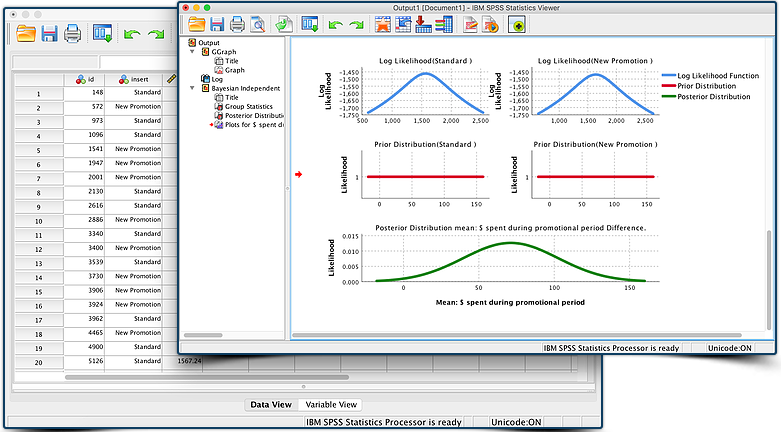
\includegraphics[width=0.9\textwidth]{SPSS.png}
      \caption{SPSS用户操作界面}
    \end{figure}}
   
  \only<4->{
    \begin{alertblock}{SPSS及其他所见即所得工具的缺陷}
      \begin{itemize} \small
        \item<4->[\PencilLeftDown] 按钮数量是有限的,而需求是无限的
        \item<5->[\PencilLeftDown] 图形要素控制缺乏灵活性和精准性
        \item<6->[\PencilLeftDown] 生成一张图易,生成N张图难
        \item<7->[\PencilLeftDown] 贫穷限制了想象力
      \end{itemize}
    \end{alertblock}}
\end{overlayarea}
\end{frame}

\subsection{所想即所得工具}
\subsubsection{SAS}
\begin{frame}[t]{\subsecname}{\subsubsecname}
  \begin{itemize}
    \item<1-> 1960年诞生于SAS软件研究所,老牌专业统计软件
    \item<2-> 基于数据库进行数据管理,具有大型数据集处理分析能力
    \item<3-> 有专门的SAS认证考试,包括程序员、业务分析师、数据挖掘、系统开发
           专家和系统管理专家五种不同角色
  \end{itemize}
  
  \begin{overlayarea} {\textwidth}{\textheight}
    \only<1-4>{
      \begin{figure}
        \centering 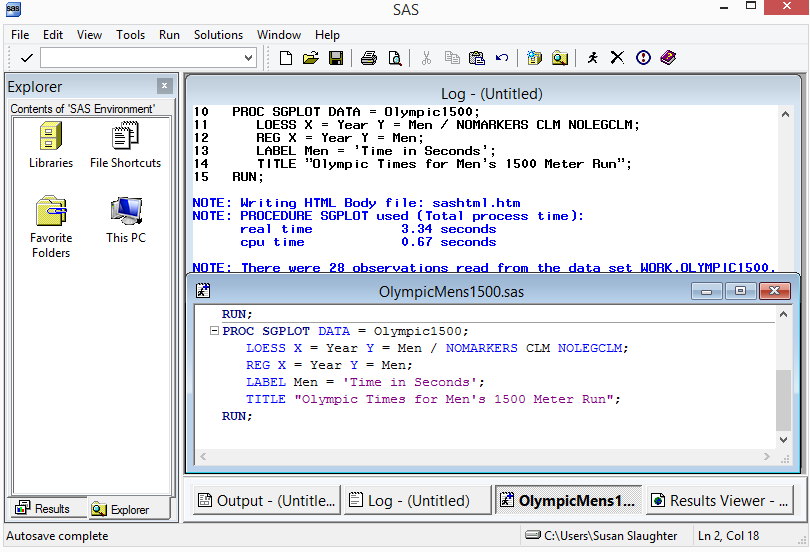
\includegraphics[width=0.7\columnwidth]{sas_ui.png}
        \caption{SAS软件界面}
      \end{figure}}
  \end{overlayarea}
\end{frame}

\begin{frame}[t, fragile]{\subsecname}{\subsubsecname}
  \begin{itemize}
    \item 200多个集成模块,涵盖了主流统计模型和分析方法,而且通过内置
           脚本语言实现统计建模和绘图等功能
  \end{itemize}
 
      \begin{columns}
        \begin{column}[c]{.5\textwidth}
          \centering 
          \begin{figure}
            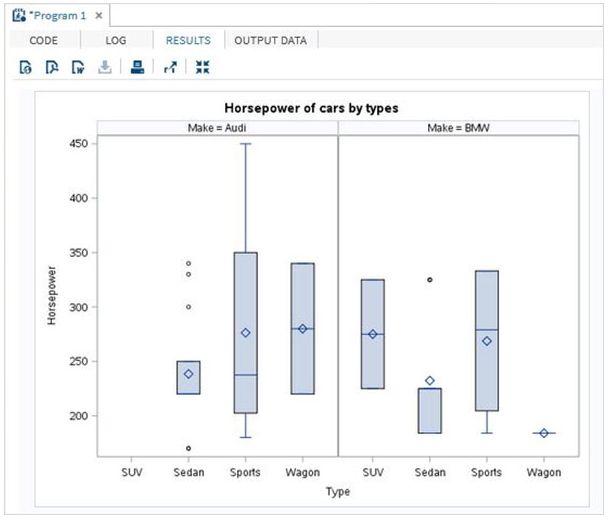
\includegraphics[width=0.8\columnwidth]{sas_boxplot.png}
            \caption{箱形图(Box plot)}
          \end{figure}
        \end{column}

        \begin{column}[c]{.5\textwidth}\centering
\begin{lstlisting}[language=SAS]
PROC SQL;
create table CARS1 as
SELECT make,model,type,invoice,horsepower,length,weight
 FROM SASHELP.CARS
WHERE make in ('Audi','BMW');
RUN;

PROC SGPLOT  DATA=CARS1;
  VBOX horsepower 
  / category = type;

   title 'Horsepower of cars by types';
RUN; 
\end{lstlisting}
        \end{column}
      \end{columns}
\end{frame}

\subsubsection{S-Plus}
\begin{frame}[t]{\subsecname}{\subsubsecname}
    \begin{itemize}
      \item S语言是1976年AT\&T贝尔实验室开发的一种用于统计计算的解释型编程语言
    \end{itemize}

    \begin{figure}
      \centering 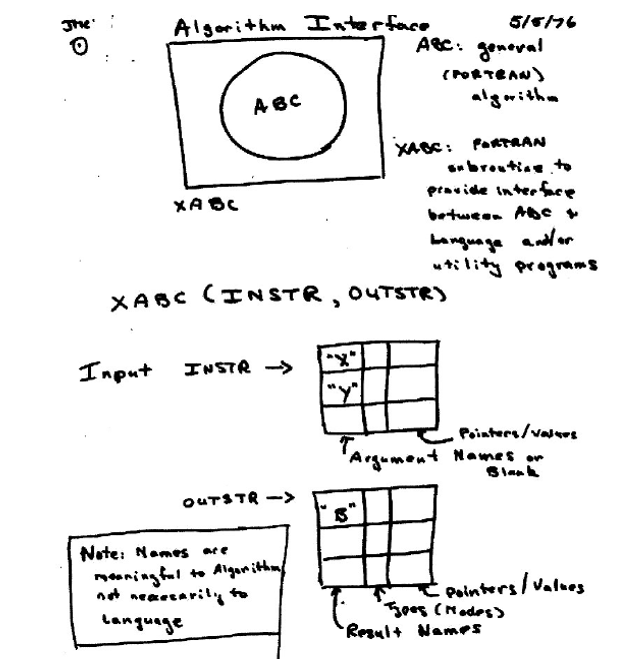
\includegraphics[width=0.5\columnwidth]{S_init.png}
      \caption{S语言的设计草图(1976.5.5)}
    \end{figure}

\end{frame}   

\begin{frame}[t, fragile]{\subsecname}{\subsubsecname}
    \begin{itemize}
      \item 与SAS内置脚本语言相比,S语言更加符合现代程序语言的设计,方便灵活控制
            图形输出,制作既精美又专业的统计图形
      \item 能够与其他主流程序语言集成
    \end{itemize}

    \begin{onlyenv}<1>
      \begin{columns}
        \begin{column}{.7\textwidth}
          \begin{figure}
            \centering
            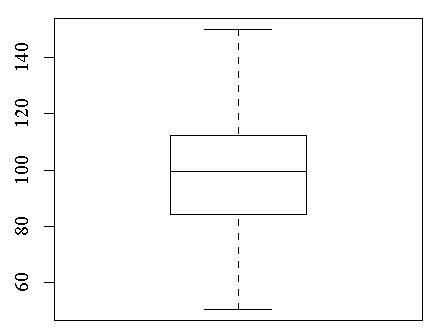
\includegraphics[width=0.8\columnwidth]{splus_boxplot.png}
            \caption{箱形图(Box plot)}
          \end{figure}
        \end{column}

        \begin{column}{.3\textwidth}
\begin{lstlisting}[language=S]
  boxplot(Weight)
\end{lstlisting}
        \end{column}
      \end{columns}
    \end{onlyenv}
\end{frame}    

\begin{frame}[t]{\subsecname}{\subsubsecname}
    \begin{itemize}
      \item S-Plus是基于S语言开发的商业化统计软件,1993年由MathSoft公司开发,
            2008年起由TIBCO负责运维
      \item 与SPSS和SAS并称世界三大统计软件,具有专业的统计功能
    \end{itemize}

    \begin{figure}
      \centering 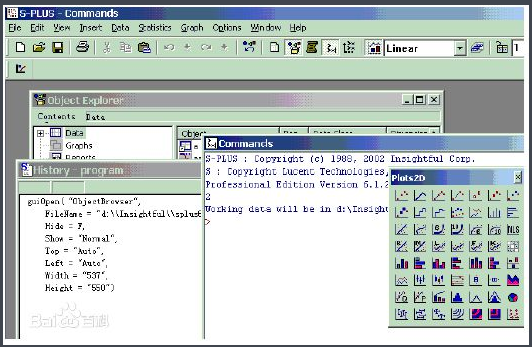
\includegraphics[width=0.8\columnwidth]{splus_ui.png}
      \caption{S-Plus软件界面}
    \end{figure}
\end{frame}    

\begin{frame}{\subsecname}{}
  % \begin{variableblock}{所想即所得工具}{bg=green!20,fg=black}{fg=white,bg=SpringGreen4}
  %   \begin{itemize}
  %   \item wowo
  %   \item sdsfs
  %   \end{itemize}
  % \end{variableblock}
\onslide<1->{
  \begin{goodbox}{所想即所得工具的优势}
     \begin{itemize}
     \item[\PencilLeftDown] 想象力有多大,世界就有多精彩
     \item[\PencilLeftDown] 花有重开日,人无再少年
     \item[\PencilLeftDown] 深入算法内核,由术至道 
     \end{itemize}
  \end{goodbox}}

\onslide<2->{
  \begin{badbox}{所想即所得工具的劣势}
     \begin{itemize}
     \item[\PencilLeftDown] 人机交互全靠指令输入,需要具备编程基础
     \item[\PencilLeftDown] 需要扎实的统计学基础,学习曲线陡峭
     \item[\PencilLeftDown] 实现简单的统计功能时不如“所见即所得工具”快捷    
     \end{itemize}
  \end{badbox}}

\end{frame} 

%
%%% Local Variables:
%%% mode: latex
%%% TeX-master: section03.tex
%%% End:
%%%%%%%%%%%%%%%%%%%%%%%%%%%%%%%%%%%%%%%%%%%%%%%%%%%%%%%%%%%
\section{R简介}
%%%%%%%%%%%%%%%%%%%%%%%%%%%%%%%%%%%%%%%%%%%%%%%%%%%%%%%%%%%%
\subsection{为什么用R}
\begin{frame}{\subsecname}{}

  \begin{columns}
    \begin{column}{.5\textwidth}
      \begin{figure}
        \centering 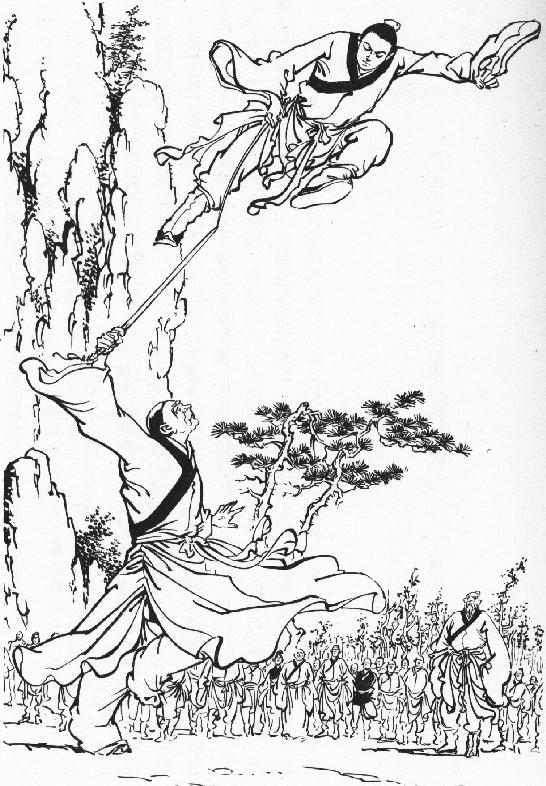
\includegraphics[width=0.9\columnwidth]{乾坤大挪移.jpg}
      \end{figure}
    \end{column}

    \begin{column}{.48\textwidth}
      \begin{ornamentblock}
        \centering
        {君子性非异也,善假于物也\\
          \rightline{\textemdash《荀子·劝学》}}
      \end{ornamentblock}
      % \curlyframe{工欲善其事,必先利其器\\
      % \rightline{-----《论语·卫灵公》}}
    \end{column}
  \end{columns}
\end{frame}

\begin{frame}[t]{\subsecname}{R的历史}

\begin{itemize}
\item<1-> R诞生于1995年,由新西兰Auckland大学统计学家\emphText{R}obert Gentleman
        和\emphText{R}oss Ihaka开发,而且完全开放源代码,是一款
        基于GNU General Public License(GPL)协议的开源软件;
由于两位开发者的名字都以“R”开头,而且为了向S语言致敬,因此命名为R
\item<2-> R是“所想即所得”工具,其核心是基于S语言设计的R语言,S语言的代码可以不经过
        任何修改就在R中运行,因此R被看做是S语言的非商业化实现  
\end{itemize}

\begin{overlayarea} {\textwidth}{\textheight}
    \begin{figure}\centering
      \captionsetup[subfigure]{labelformat=empty} 
      \subfloat[Ross Ihaka]
      {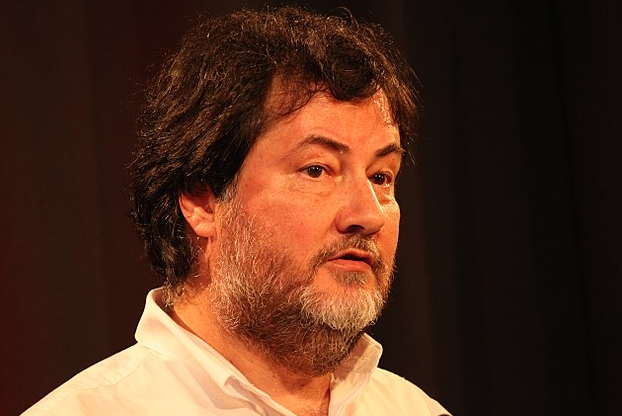
\includegraphics[width=0.45\columnwidth]{Ross_Ihaka.png}} \vspace{1pt}
      \subfloat[Robert Gentleman]
      {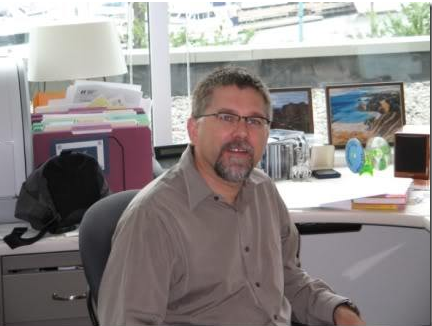
\includegraphics[width=0.4\columnwidth]{Robert_Gentleman.png}} 
    \end{figure}
\end{overlayarea}

\end{frame}

\begin{frame}[t]{\subsecname}{R的优势}
\begin{itemize}
\item<1-> R具备S-Plus几乎所有的优点,而且更加小巧轻便
\item<2-> 开源项目,完全免费,这点是其他统计软件都不具备的
\item<3-> 世界各地有大量研究机构和专业统计人员使用
                 并自愿贡献代码,具有良好的生态系统
\end{itemize}  

\begin{overlayarea}{\textwidth}{\textheight}

\only<1-2>{
  \begin{figure}[ht]
    \centering
    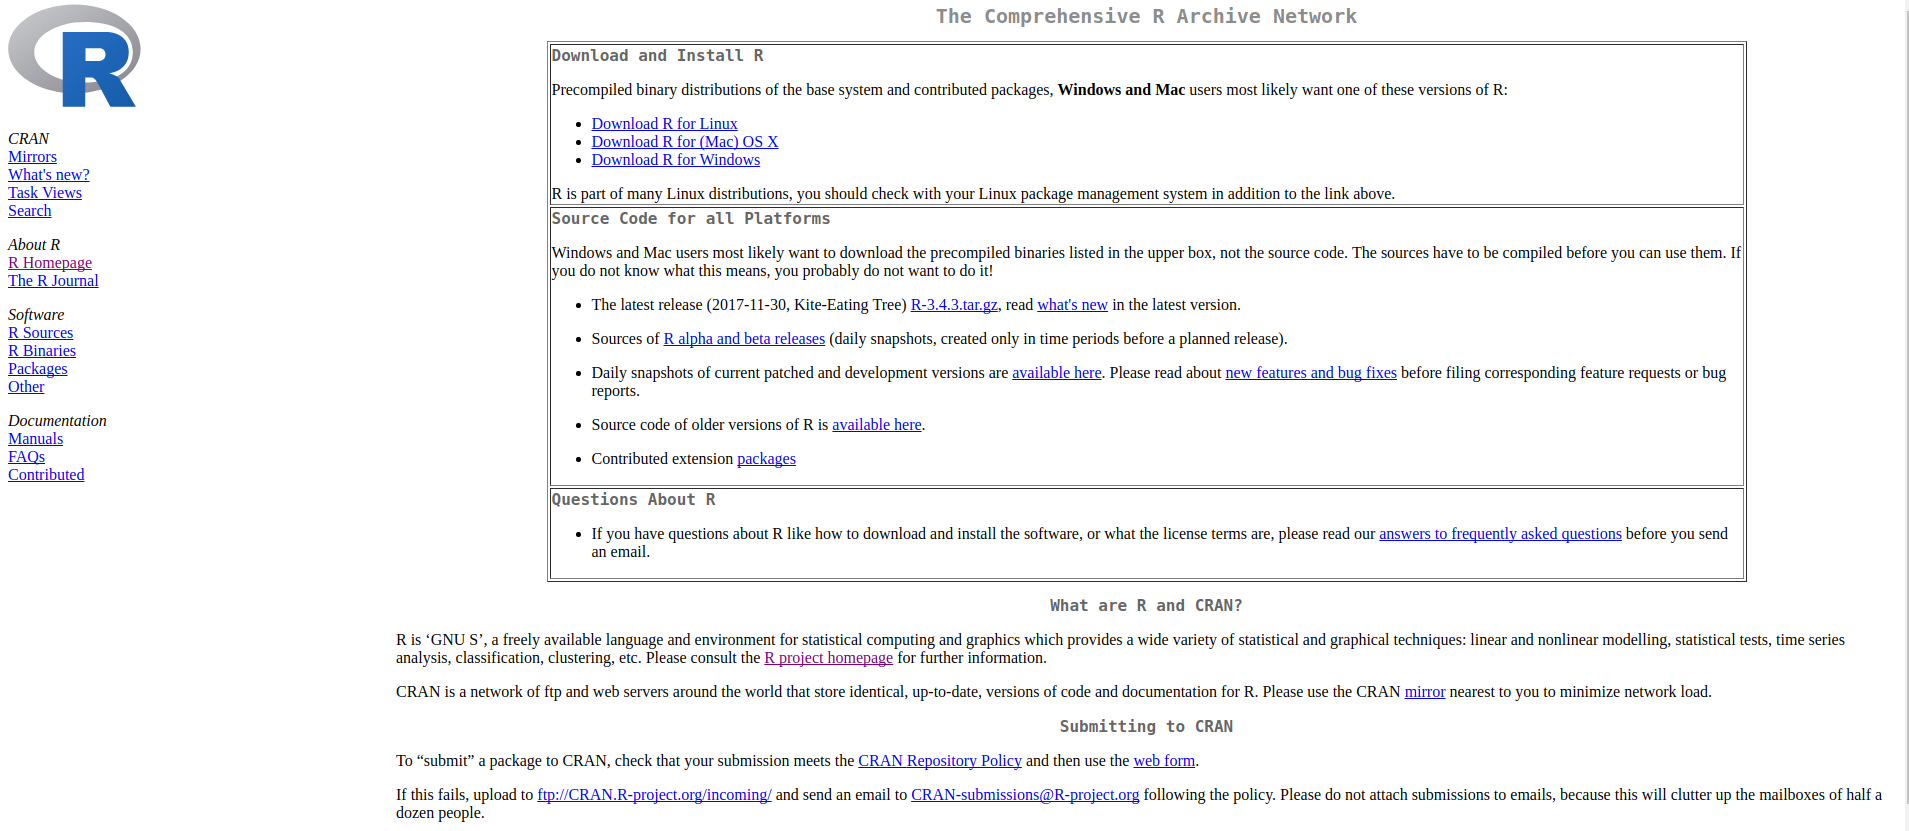
\includegraphics[width=\columnwidth]{CRAN.png}
    \caption{R的官方网站CRAN(https://cran.r-project.org/)}
  \end{figure}}

\only<3->{
  \begin{figure}[ht]
    \centering
    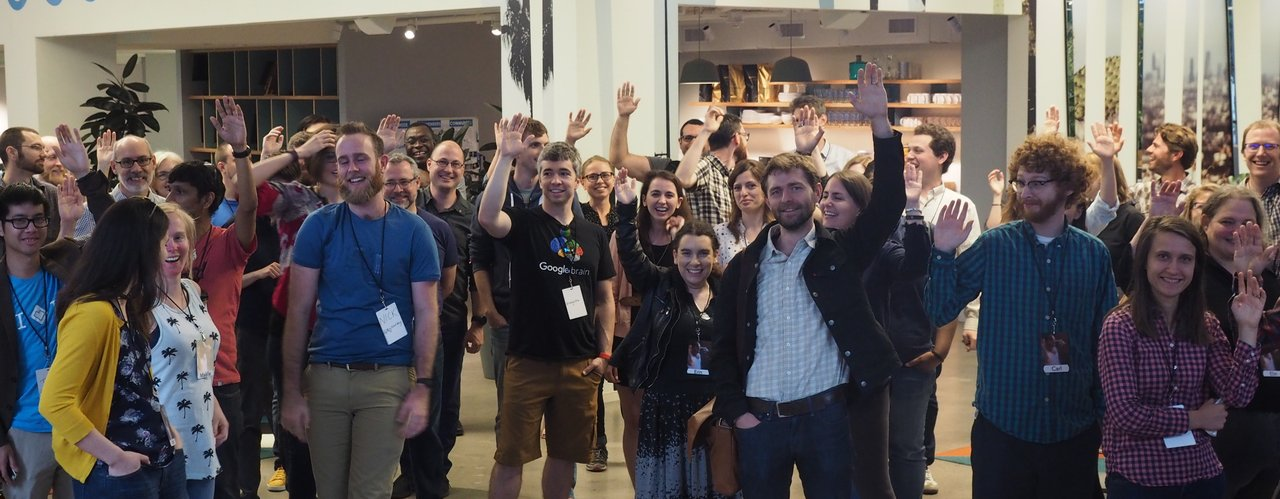
\includegraphics[width=\columnwidth]{R_community.jpg}
    \caption{来自世界各地R的无私贡献者们}
  \end{figure}}
\end{overlayarea}

\end{frame} 

\begin{frame}[t]{\subsecname}{R的优势}
\begin{itemize}
\item<1-> R是高度模块化软件,通过程序包(package)来扩展其功能;目前CRAN上
                 的程序包超过12000个,绝大多数来自自愿者的贡献
\item<2-> R语言语法简单,不需要很高的编程技巧,而且与其他语言具有极好的兼容性
\item<3-> 几乎所有的统计模型都有R语言的实现版本,因此与统计研究前沿相接轨 
\end{itemize}  

\begin{overlayarea}{\textwidth}{\textheight}
\only<1>{
  \begin{figure}[ht]
    \centering
    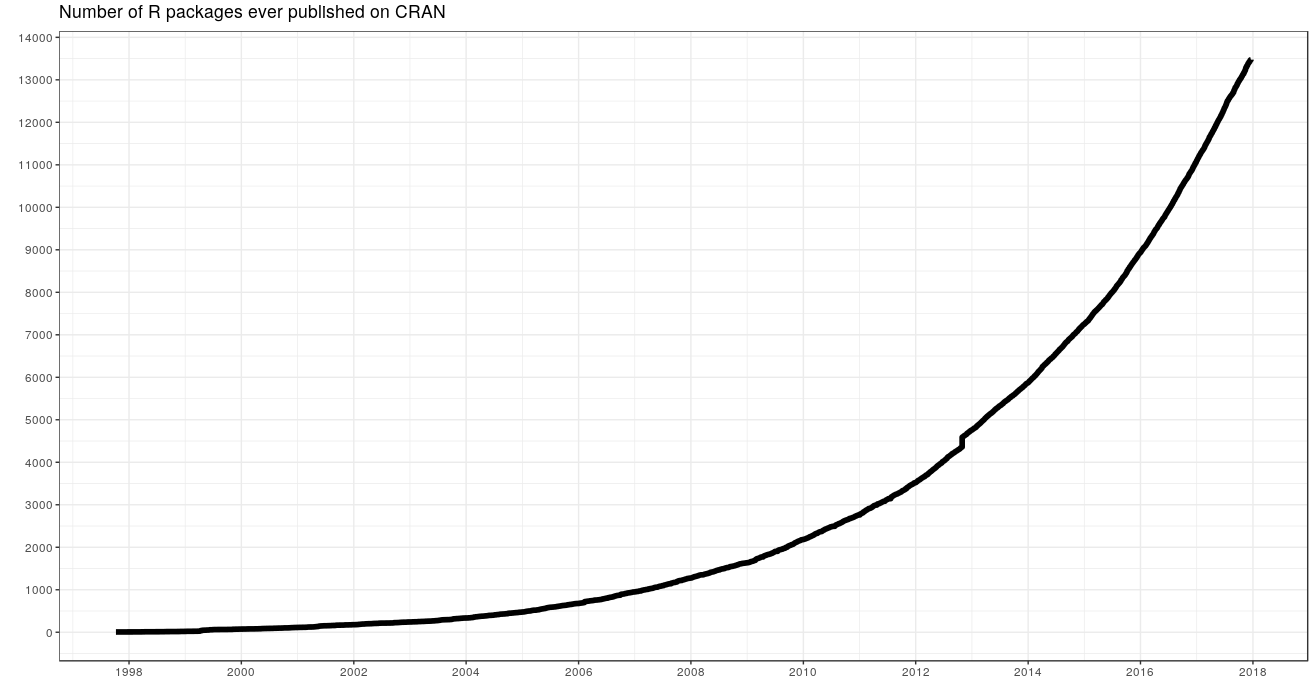
\includegraphics[width=0.7\columnwidth]{number_of_R_packages.png}
    \caption{历年R packages提交的数量统计}
  \end{figure}}

\only<2>{
\begin{block}{R语言的兼容性}
  \begin{itemize}
  \item[\PencilLeftDown] \emphText{内部兼容}:由于R语言本身是解释性语言,
    执行效率较低,因此R的底层函数有很大一部分代码是C语言和Fortran语言编
    写的
  \item[\PencilLeftDown] \emphText{外部兼容}:目前主流的编程语言,例
    如JAVA、c++、python等几乎都有相应的程序库来调用R语言编写的程序,来
    帮助这些编程语言简化统计计算和绘图相关的功能
  \end{itemize}
\end{block}}

\only<3>{
  \begin{figure}
    \centering
    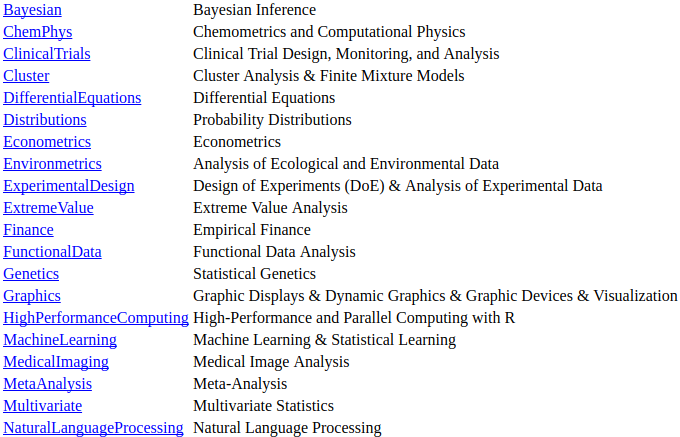
\includegraphics[width=0.55\columnwidth]{CRAN_TASK1.png}
    \caption{R packages的任务分类}
  \end{figure}}

\only<4>{
  \begin{figure}
    \centering
    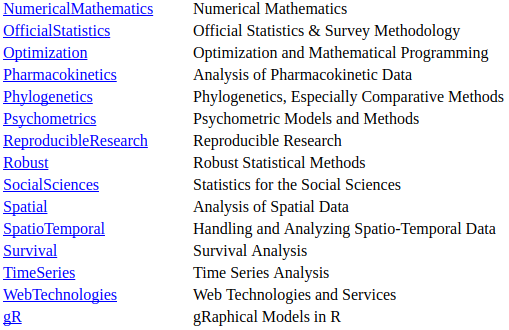
\includegraphics[width=0.55\columnwidth]{CRAN_TASK2.png}
    \caption{R packages的任务分类}
  \end{figure}}
\end{overlayarea}

\end{frame} 

\subsection{基础知识}
\begin{frame}[shrink]{\subsecname}{R的工作原理}
\begin{itemize}
\item 在R中进行的所有操作都是针对存储在\emphText{内存中的对象}
\item 用户通过输入命令调用函数,\emphText{分析结果可以被直接显示在屏幕上,也可以被存入某个对象或被
写入硬盘}(如图片对象)
\item 因为分析结果本身也是对象,所以它们也能\emphText{被视为数据并能像一般数据那样被处理分析}
\item 数据可以从本地磁盘读取,也可从远程服务器端获得 
\end{itemize} 

\begin{figure}[ht]
  \centering
  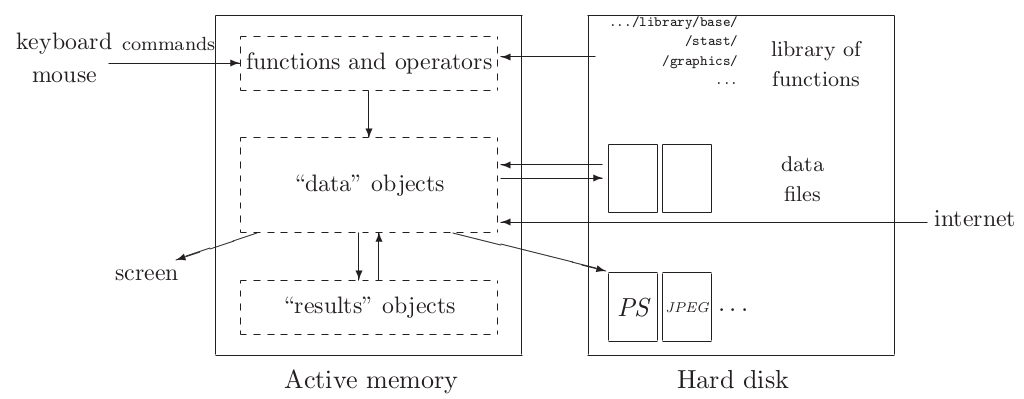
\includegraphics[width=0.9\columnwidth]{R_principle.png}
  \caption{R的工作原理}
\end{figure}
\end{frame}

\begin{frame}[t]{\subsecname}{安装运行环境}
\begin{itemize}
\item R的主安装程序由自愿者进行编译上传,基本上每个在CRAN上可以自由下载,包括windows、linux
                 和mac三大主流平台
\item 安装后的程序界面是一个交互式命令行终端,默认由一个“>”符号表示命令输入和结果
                 输出指示符
\item 在windows有一个简陋的GUI,linux和mac下默认只有CLI终端 
\end{itemize} 

\begin{overlayarea}{\textwidth}{\textheight}
\only<1>{
  \begin{figure}[ht]
    \centering
    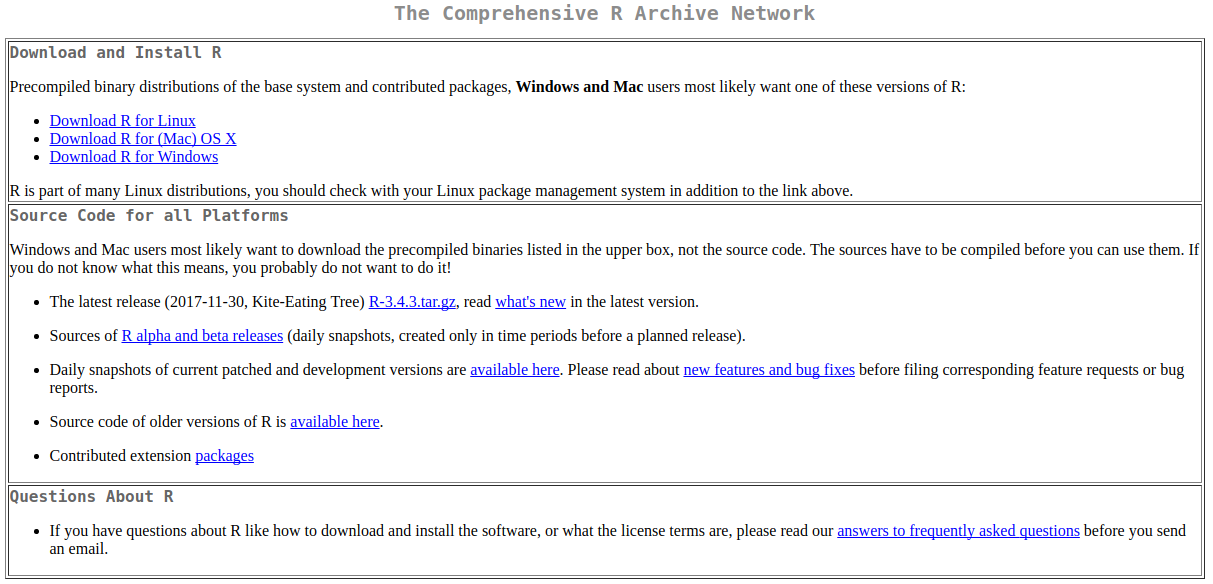
\includegraphics[width=0.8\columnwidth]{R_download.png}
    \caption{R在CRAN的下载界面}
  \end{figure}}

\only<3>{
  \begin{figure}[ht]
    \centering
    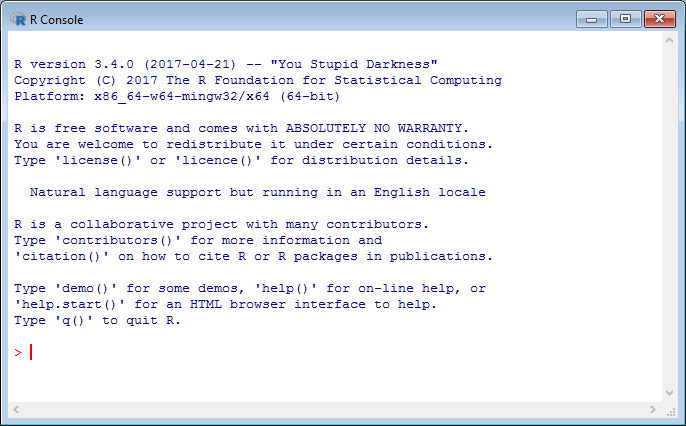
\includegraphics[width=0.6\columnwidth]{R_gui.png}
    \caption{R在windows下的GUI}
  \end{figure}}

\only<4>{
  \begin{figure}[ht]
    \centering
    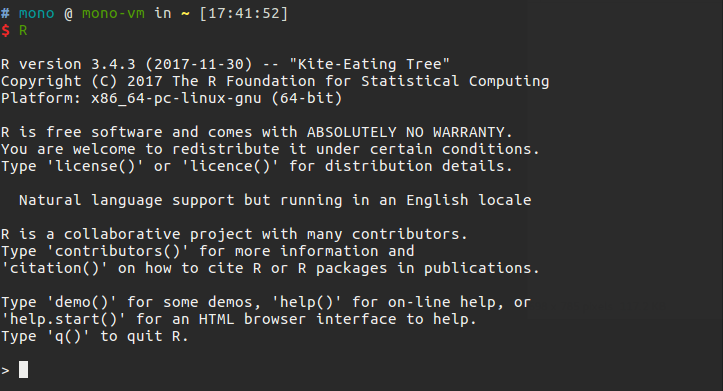
\includegraphics[width=0.7\columnwidth]{R_cli.png}
    \caption{R在linux下的cli终端}
  \end{figure}}
\end{overlayarea}
\end{frame}

\begin{frame}[t, fragile]{\subsecname}{基本操作}
\begin{itemize}
  \item R的第一种操作就是\emphText{“输入命令$\rightarrow$回车$\rightarrow$输出结果”}这种
             标准的交互式命令行方式  
\end{itemize} 

\begin{overlayarea}{\textwidth}{\textheight}
\begin{onlyenv}<1>
\begin{rcode}
> x = runif(100); y = 0.2*x + 0.1*rnorm(100)
> fit = lm(y ~ x)
> summary(fit)

Call:
lm(formula = y ~ x)

Residuals:
     Min       1Q   Median       3Q      Max 
-0.30665 -0.05002 -0.01135  0.06047  0.24599 

Coefficients:
            Estimate Std. Error t value Pr(>|t|)    
(Intercept)  0.02052    0.01670   1.229    0.222    
x            0.17510    0.03107   5.636 1.67e-07 ***
---
Signif. codes:  0 ‘***’ 0.001 ‘**’ 0.01 ‘*’ 0.05 ‘.’ 0.1 ‘ ’ 1

Residual standard error: 0.08959 on 98 degrees of freedom
Multiple R-squared:  0.2448,    Adjusted R-squared:  0.2371 
F-statistic: 31.77 on 1 and 98 DF,  p-value: 1.671e-07
\end{rcode}
\end{onlyenv}

\begin{onlyenv}<2>
\begin{rcode}
plot(x, y); abline(fit)
\end{rcode}
\begin{figure}
    \centering
    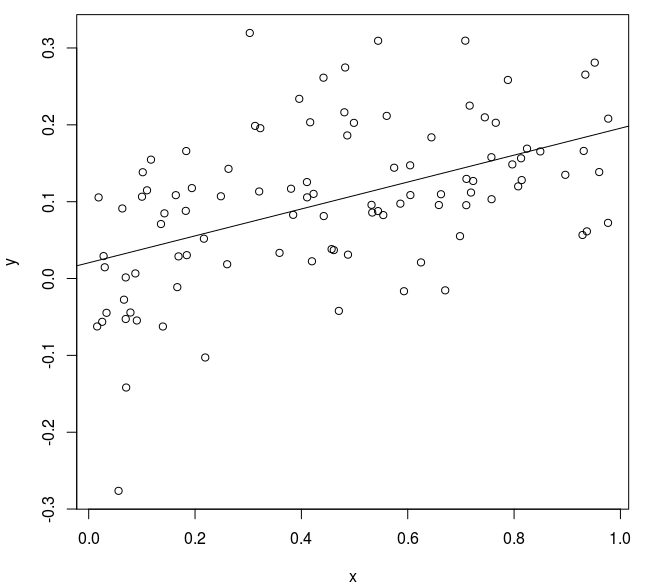
\includegraphics[width=0.55\columnwidth]{R_output.png}
\end{figure}
\end{onlyenv}
\end{overlayarea}
\end{frame}

\begin{frame}[t, fragile]{\subsecname}{基本操作}
\begin{itemize}
\item<1-> 第二种方式是将脚本代码写在文件中,然后一次性运行
\item<2-> 如果代码量很大建议使用第二种方式,因为文件比较容易修改和保存,而且目前
        有专用IDE可以辅助编写R脚本代码  
\end{itemize} 

\begin{overlayarea}{\textwidth}{\textheight}
\only<1>{
  \begin{figure}[ht]
    \centering
    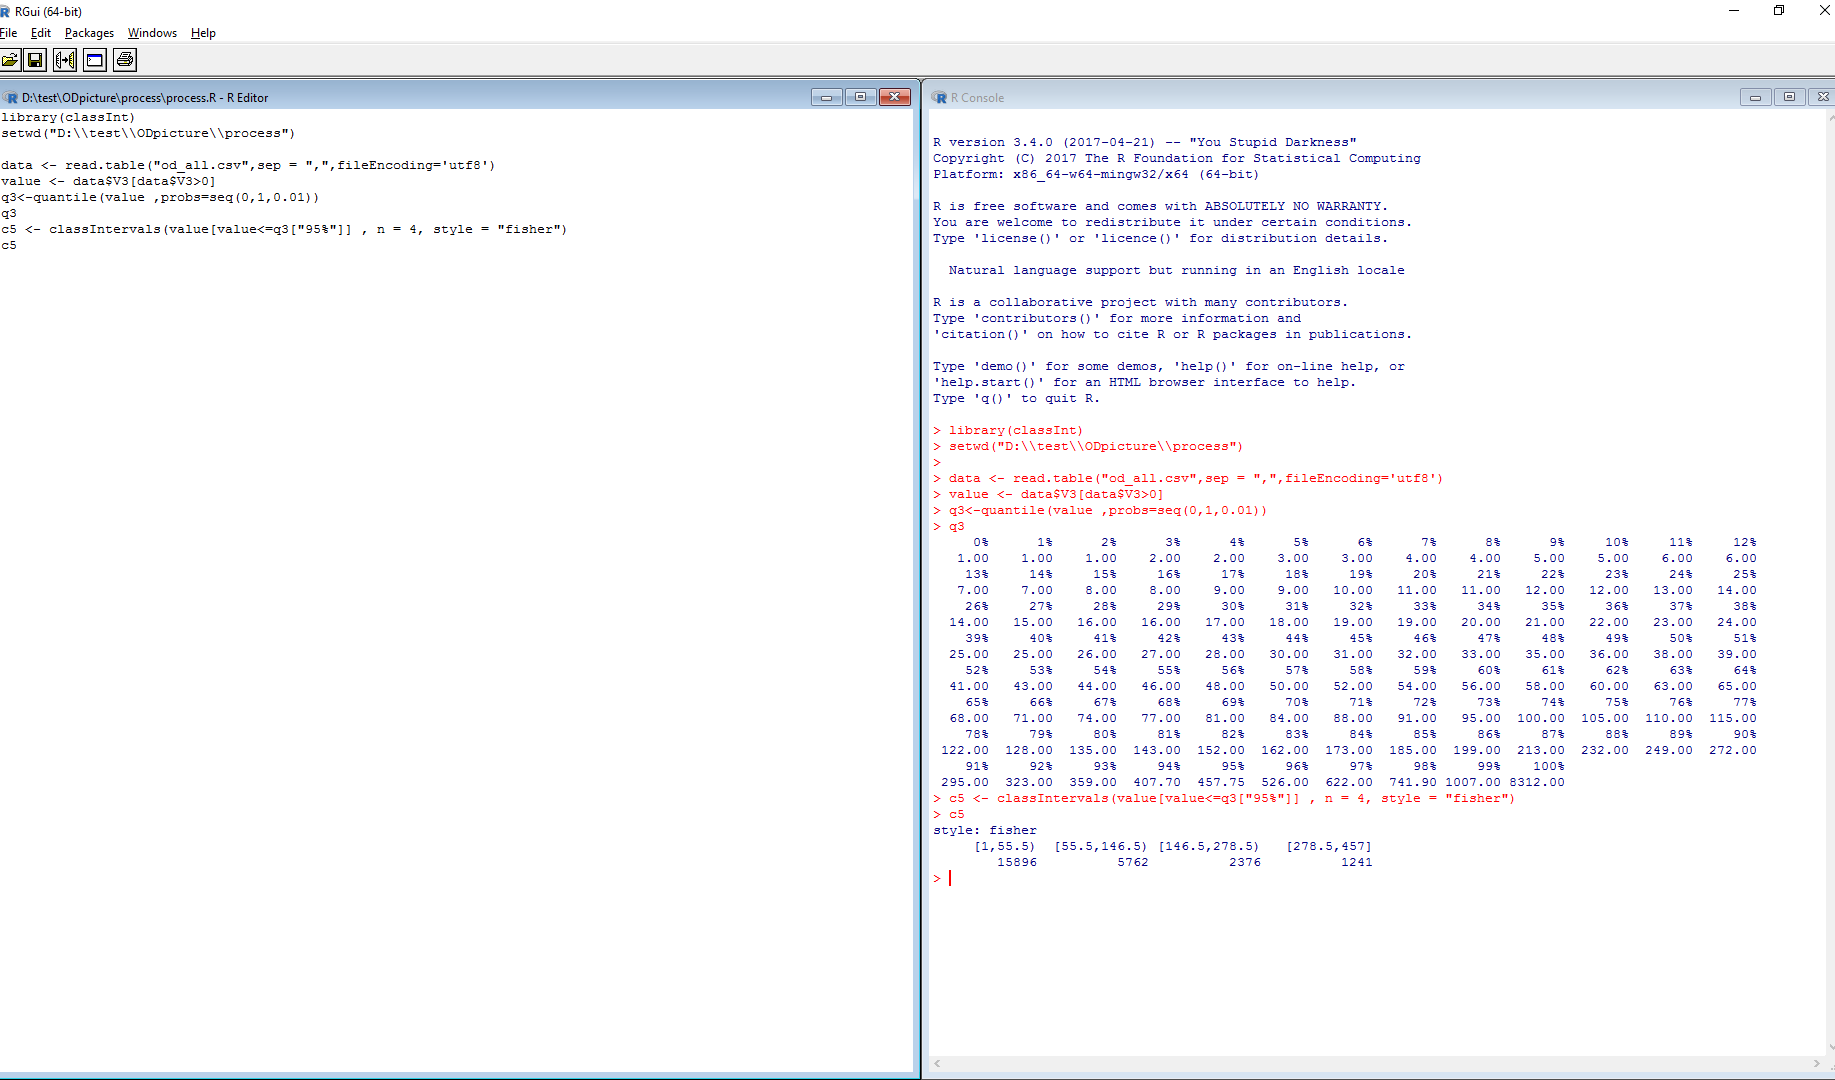
\includegraphics[width=0.8\columnwidth]{R_editor.png}
    \caption{在文本编辑器中编写脚本,然后一次性在终端运行}
  \end{figure}}   

\only<2>{
  \begin{figure}[ht]
    \centering
    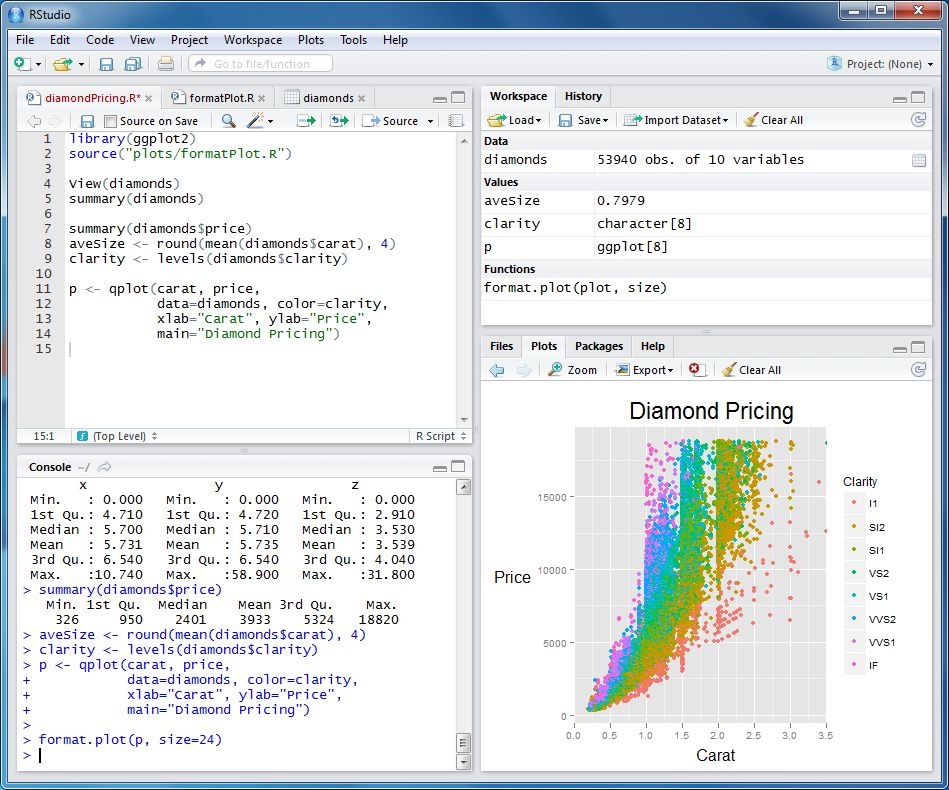
\includegraphics[width=0.6\columnwidth]{RStudio.jpg}
    \caption{\emphText{RStudio}是目前最专业的R IDE,具有大量针对R语言特点设计的功能,
             而且个人桌面版完全开源,可以免费使用}
  \end{figure}}   
\end{overlayarea}
\end{frame}

\begin{frame}[t]{\subsecname}{程序包}
\begin{itemize}
\item<1-> R的程序包分为\emphText{base包}和\emphText{contrib包}
\item<2-> base包是安装R的时候就自带的,不需要单独安装,
    这类包的质量都非常高,性能稳定
\item<3-> contrib包是自愿者上传的,质量参次不齐;其中质量好
    且用户量大的扩展包有可能会纳入下一个版本的主程序包
\end{itemize}

\begin{overlayarea}{\textwidth}{\textheight}
\only<1>{
  \begin{figure}[h]
    \centering
    
\includegraphics[width=\columnwidth]{R_packages.png}
    \caption{CRAN上下载base包和contrib包}
  \end{figure}}  

\only<2>{
  \begin{table} \centering \small
    \begin{tabular}{|c|c|}
      \toprule
      \rowcolor{LightCyan}
      名称 & 用途\\\hline
      base & R基础函数包\\\hline
      methods & 用于 R 对象和编程工具的方法和类的定义\\\hline
      datasets & R通用数据集\\\hline
      graphics & 基础统计绘图包 \\\hline
      utils & 通用函数包 \\\hline
      stats & 基础统计计算包 \\\hline
      grDevices & 基础或grid图形设备\\
      \bottomrule
    \end{tabular}
    \caption{常用的base包}
  \end{table}}

\only<3>{
  \begin{table} \centering \small 
    \begin{tabular}{|c|c|}
      \toprule
      \rowcolor{LightCyan}
      名称 & 用途\\\hline
      cluster & 聚类分析包\\\hline
      maptools & 空间数据读取和处理包\\\hline
      spatstat & 空间点数据分析包\\\hline
      sp & 空间数据基础类包\\\hline
      spdep & 空间自相关模型包\\\hline
      ggplot2 & 基于绘图语法的数据可视化包 \\\hline
      knitr & R文学编程包 \\\hline
      \bottomrule
    \end{tabular}
    \caption{常用的contrib包}
  \end{table}}
\end{overlayarea}
\end{frame}

\begin{frame}[t,fragile]{\subsecname}{程序包}
\begin{itemize}
\item<1-> base包在R启动之后自动加载,可以直接使用;而contrib包则需要通过library函数调用,如果未安装
               相应包则会报错
\item<2-> 通过\emphTextStep{2-}{install.packages}函数安装contrib包
\end{itemize}

\begin{overlayarea}{\textwidth}{\textheight}
\begin{onlyenv}<1->
\begin{rcode}
> library(sp)
Error in library(sp) : there is no package called ‘sp’
\end{rcode}
\end{onlyenv}

\begin{onlyenv}<2>
\begin{rcode}
> install.packages("sp")
Installing package into ‘/home/mono/Softwares/R/3.4’
(as ‘lib’ is unspecified)
--- Please select a CRAN mirror for use in this session ---
trying URL 'http://mirrors.tuna.tsinghua.edu.cn/CRAN/src/contrib/sp_1.2-6.tar.gz'
Content type 'application/octet-stream' length 1133739 bytes (1.1 MB)
==================================================
downloaded 1.1 MB

* installing *source* package ‘sp’ ...
\end{rcode}
\end{onlyenv}
\end{overlayarea}
\end{frame}

\begin{frame}[t,fragile]{\subsecname}{帮助系统}
\begin{itemize}
\item<1-> 通过\emphTextStep{1-}{?命令}或者\emphTextStep{1-}{help函数}
               查看程序包中函数的本地帮助文档
\item<2-> 通过\emphTextStep{2-}{help.search函数}在整个帮助系统中进行关键字搜索
\item<3-> \emphTextStep{3-}{find函数}可以根据名称精确查找对象,
               \emphTextStep{3-}{apropos函数}可以根据名称模糊查找对象
\end{itemize}

\begin{overlayarea}{\textwidth}{\textheight}
\begin{onlyenv}<1>
\begin{rcode}
> ?lm
lm               package:stats            R Documentation

Fitting Linear Models

Description:

     ‘lm’ is used to fit linear models.  It can be used to carry out regression, single stratum analysis of variance and analysis of covariance (although ‘aov’ may provide a more convenient interface for these).

Usage:

     lm(formula, data, subset, weights, na.action, method = "qr", model = TRUE, x = FALSE, y = FALSE, qr = TRUE, singular.ok = TRUE, contrasts = NULL, offset, ...)
\end{rcode}
\end{onlyenv}

\begin{onlyenv}<2>
\begin{rcode}
> help.search("data input")
Help files with alias or concept or title matching ‘data input’ using fuzzy matching:


utils::read.DIF         Data Input from Spreadsheet
utils::read.table       Data Input


Type '?PKG::FOO' to inspect entries 'PKG::FOO', or 'TYPE?PKG::FOO' for entries like 'PKG::FOO-TYPE'.
\end{rcode}
\end{onlyenv}

\begin{onlyenv}<3>
\begin{rcode}
> find("lm")
[1] "package:stats"
> appropos("lm")
 [1] "colMeans"        ".colMeans"       "confint.lm"      "contr.helmert"  
 [5] "dummy.coef.lm"   "getAllMethods"   "glm"             "glm.control"    
 [9] "glm.fit"         "KalmanForecast"  "KalmanLike"      "KalmanRun"      
[13] "KalmanSmooth"    "kappa.lm"        "lm"              ".lm.fit"        
[17] "lm.fit"          "lm.influence"    "lm.wfit"         "model.matrix.lm"
[21] "nlm"             "nlminb"          "predict.glm"     "predict.lm"     
[25] "residuals.glm"   "residuals.lm"    "summary.glm"     "summary.lm" 
\end{rcode}
\end{onlyenv}

\end{overlayarea}
\end{frame}

\subsection{数据操作}
\begin{frame}[t]{\subsecname}{对象(object)}
  \begin{itemize}
  \item R语言中操作的实体在技术上来说就是对象(object) 
  \item 语言中使用对象的好处是可以复用,提升自动化程度
  \item R的所有对象有两个内在属性:类型(mode)和长度(length)
  \end{itemize}

  \begin{columns}
    \begin{column}{.5\textwidth}
      \begin{figure}
        \centering 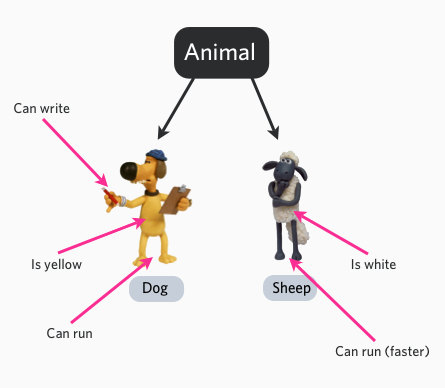
\includegraphics[width=\columnwidth]{object.png}
      \end{figure}
    \end{column}

    \begin{column}{.48\textwidth}
      \begin{ornamentblock}
        \centering
        {在R语言中,\emphText{几乎任何东西都是对象}}
      \end{ornamentblock}
    \end{column}
  \end{columns}
\end{frame}

\begin{frame}[t, fragile]{\subsecname}{数据类型(mode)}
  \begin{itemize}
  \item 实数型(real):整数(integer)、单精度(single)、双精度(double)
  \item 虚数型(complex):如10+21i
  \item 字符型(character, string):如"hello world"
  \item 逻辑型(logical):TRUE(可以简写成T),FALSE(可以简写成F)
  \item 函数(function)
  \item 表达式(expression)
  \end{itemize}

\begin{overlayarea}{\textwidth}{\textheight}
\begin{rcode}
> x <- 1
> mode(x)
[1] "numeric"
> length(x)
[1] 1
> A <- "Gomphotherium"; compar <- TRUE; z <- 1i
> mode(A); mode(compar); mode(z)
[1] "character"
[1] "logical"
[1] "complex"
# 表达式
> x <- 3; y <- 2.5; z <- 1
> exp1 <- expression(x / (y + exp(z)))
> exp1
expression(x/(y + exp(z)))
> eval(exp1)
[1] 0.5749019
\end{rcode}
\end{overlayarea}
\end{frame}

\begin{frame}[t]{\subsecname}{数据结构}
  \begin{itemize}
  \item R语言中为了提高数据的使用效率,预定义了专门用于表示数据的对象,也就是数据结构,这些数据结构支撑了R强大的统计分析能力
  \end{itemize}
% \only<1>{
%   \begin{ornamentblock}[userdefinedwidth=0.6\textwidth,align=center]
%         \centering
%         {Everything in R is an object\\
%          Every object in R has a class}
%       \end{ornamentblock}}
  \begin{table} \centering \small
    \begin{tabular}{|c|c|}
      \toprule
      \rowcolor{LightCyan}
      数据结构 & 类型\\\hline
      向量(vector) & 数值型,字符型,复数型,逻辑型\\\hline
      因子(factor) & 数值型,字符型\\\hline
      数组(array) & 数值型,字符型,复数型,逻辑型\\\hline
      矩阵(matrix) & 数值型,字符型,复数型,逻辑型 \\\hline
      数据框(data.frame) & 数值型,字符型,复数型,逻辑型 \\\hline
      列表(list) & 任意其他类型 \\\hline
      时间序列(ts) & 数值型,字符型,复数型,逻辑型\\
      \bottomrule
    \end{tabular}
    \caption{R基础数据结构}
  \end{table}
\end{frame}

\begin{frame}[t,fragile]{\subsecname}{数据结构}
  \frametitle{}{向量(vector)}
  \begin{itemize}
  \item \emphText{向量是R中最基本的数据单元},向量中的对象类型必须相同
  \item 构建向量常用的函数: rep()、c()、seq()、cbind()、rbind()等
  \item \emphText{向量的下标从1开始},这和其他计算机高级编程语言是不一样的!
  \end{itemize}  

%\begin{overlayarea}{\textwidth}{\textheight}
\begin{rcode}
> x <-1:10; x
[1]  1  2  3  4  5  6  7  8  9 10
> x[3]
[1] 3
> c(7.11, 9.11, 9.19, 1.23)
[1] 7.11 9.11 9.19 1.23
> c("B", "A")
[1] "B" "A"
> rep(1, 10)
[1] 1 1 1 1 1 1 1 1 1 1
> seq(1, 5, 0.5)
[1] 1.0 1.5 2.0 2.5 3.0 3.5 4.0 4.5 5.0
> cbind(0, rbind(1, 1:3))
     [,1] [,2] [,3] [,4]
[1,]    0    1    1    1
[2,]    0    1    2    3
\end{rcode}  
%\end{overlayarea}
\end{frame}

\begin{frame}[t,fragile]{\subsecname}{数据结构}
  \frametitle{}{因子(factor)}
  \begin{itemize}
  \item 因子是对应统计学中的分类数据(categorical data)而设计的
  \item 因子形式上是一个对等长的向量元素进行分类(分组)的向量对象
  \item 因子数据具有水平(level)和标签(label),前者即分类变量的不同取
值,后者即各类取值的名称
  \end{itemize}  

\begin{rcode}
> factor(1:3, labels=c("A", "B", "C"))
[1] A B C
Levels: A B C
> (x = factor(c(1, 2, 3, 1, 1, 3, 2, 3, 3), levels = 1:3,
+   labels = c("g1", "g2", "g3")))
[1] g1 g2 g3 g1 g1 g3 g2 g3 g3
Levels: g1 g2 g3
\end{rcode}  
\end{frame}

\begin{frame}[t,fragile]{\subsecname}{数据结构}
  \frametitle{}{数组(array)和矩阵(matrix)}
  \begin{itemize}
  \item 数组和矩阵是具有维度属性(dimension)的数据结构,
        实质是有附加属性(维数dim)的向量
  \item 矩阵是数组的特例,它的维度为2,用来指定行数和列数
  \end{itemize}  

\begin{rcode}
# 二维矩阵
> matrix(data=5, nr=2, nc=2)
     [,1] [,2]
[1,]    5    5
[2,]    5    5
# 三维数组
> array(1:24, c(3, 4, 2))
, , 1
     [,1] [,2] [,3] [,4]
[1,]    1    4    7   10
[2,]    2    5    8   11
[3,]    3    6    9   12

, , 2
     [,1] [,2] [,3] [,4]
[1,]   13   16   19   22
[2,]   14   17   20   23
[3,]   15   18   21   24
\end{rcode}  
\end{frame}

\begin{frame}[t,fragile]{\subsecname}{数据结构}
  \frametitle{}{列表(list)}
  \begin{itemize}
  \item 列表是一种灵活的数据结构,\emphText{用于生成包含不同类型对象的集合}
  \end{itemize}  

\begin{rcode}
# 创建list
> x <- 1:4; y <- 2:4; L1 <- list(A=x, B=y); L1
$A
[1] 1 2 3 4

$B
[1] 2 3 4
# list元素的引用
> L1[[1]]
[1] 1 2 3 4
> L1["A"]
$A
[1] 1 2 3 4
> L1[["A"]]
[1] 1 2 3 4
> L1$B
[1] 2 3 4
\end{rcode}  
\end{frame}

\begin{frame}[t,fragile]{\subsecname}{数据结构}
  \frametitle{}{数据框(data.frame)}
  \begin{itemize}
  \item 数据框是由许多向量组成的一个二维的对象,主要用于保存建模所需要的数据
  \item 数据框的实质是一个“整齐的”列表,它只要求各列内的数据类型相同,而列之间的可以不同
  \item \emphText{数据框是R中最重要的一种数据结构},大多数数据都是以数据框形式输到R中的
  \end{itemize}  

\begin{rcode}
# 创建数据框
# 数据框中的向量必须有相同的长度,如果其中有一个比其它的短,它将“循环”整数次(以使得其长度与其它向量相同)
> x <- 1:4; M <- c(10, 35); y <- 2:4
> data.frame(x, M)
  x  M
1 1 10
2 2 35
3 3 10
4 4 35
> data.frame(x, y)
Error in data.frame(x, y) :
   arguments imply differing number of rows: 4, 3
\end{rcode}  
\end{frame}

\begin{frame}[t,fragile]{\subsecname}{表达式(expression)}
  \begin{itemize}
  \item 表达式类型对象在R中有着很基础的地位,是R能够解释的字符序列
  \item \emphText{所有有效的R命令都是表达式},表达式分为\emphText{求值表达式和非求值表达式}
  % \item 当命令从被键盘输入后,它就将被R求值,如果是有效命令则会被R解释器执行,因此\emphText{R中
% 有效命令默认都是求值表达式};但是有些情况,需要构造非求值表达式,比如将公式作为函数参数进行传递,
% 或者在图形绘制数学公式等
  \item \emphText{R中有效命令默认都是求值表达式},可以在终端直接输入,
也可以用\emphText{eval()函数}执行;而非求值表达式通过\emphText{expression()函数}执行
  \end{itemize}  

\begin{overlayarea}{\textwidth}{\textheight}
\begin{onlyenv}<2>
\begin{rcode}
> x <- 3; y <- 2.5; z <- 1
# 创建非求值表达式
> exp1 <- expression(x / (y + exp(z)))
> exp1
expression(x/(y + exp(z)))
# 执行求值表达式
> eval(exp1)
[1] 0.5749019
\end{rcode}  
\end{onlyenv}

\begin{onlyenv}<3>
\begin{columns}
  \begin{column}[c]{.5\textwidth}
\begin{figure}
  \includegraphics[width=0.8\columnwidth]{expression-example.png}
\end{figure}
  \end{column}

  \begin{column}[c]{.5\textwidth}
\begin{rcode}
> plot(1:10, 1:10)
> text(4, 9, expression(hat(beta) == (X^t * X)^{-1} * X^t * y))
> text(4, 8.4, "expression(hat(beta) == (X^t * X)^{-1} * X^t * y)", cex = .8)
> text(4, 7, expression(bar(x) == sum(frac(x[i], n), i==1, n)))
> text(4, 6.4, "expression(bar(x) == sum(frac(x[i], n), i==1, n))", cex = .8)
> text(8, 5, expression(paste(frac(1, sigma*sqrt(2*pi)), " ", plain(e)^{frac(-(x-mu)^2, 2*sigma^2)})), cex = 1.2)
\end{rcode}  
  \end{column}
\end{columns}
\end{onlyenv}
\end{overlayarea}
\end{frame}

\begin{frame}[t,fragile]{\subsecname}{数据输入输出}
\begin{itemize}
\item<1-> R的数据可以按照数据结构手动输入,也可以通过读取外部文件自动输入
\item<2-> R base包提供了文本文件(ASCII)的读取函数:\emphTextStep{2-}{read.table}、
                     \emphTextStep{2-}{scan}和\emphTextStep{2-}{read.fwf}等
\item<3-> R base包也提供了文本文件(ASCII)的输出函数:\emphTextStep{2-}{write.table}
\item<4-> 另外,\emphTextStep{4-}{图形作为对象也可以输出},这将在后面会专门介绍
\end{itemize}

\begin{overlayarea}{\textwidth}{\textheight}
\begin{onlyenv}<2>
%\begin{minted}{R}
\begin{rcode}
# 从外部读取data.dat文件,并且将数据赋给一个名为mydata的对象,这里mydata是一个data.frame数据结构
> mydata <- read.table("data.dat")

# read.table的参数
read.table(file, header = FALSE, sep = "", quote = "\"’", dec = ".", row.names, col.names, as.is = FALSE, na.strings = "NA",colClasses = NA, nrows = -1,skip = 0, check.names = TRUE, fill =!blank.lines.skip,strip.white = FALSE, blank.lines.skip = TRUE,comment.char = "#")
\end{rcode}
%\end{rcode}
\end{onlyenv}

\begin{onlyenv}<3>
\begin{rcode}
# 函数write.table可以在文件中写入一个对象,一般是写一个数据框,也可以是其它类型的对象
write.table(x, file = "", append = FALSE, quote = TRUE, sep = " ", eol = "\n", na = "NA", dec = ".", row.names = TRUE, col.names = TRUE, qmethod = c("escape", "double"))
\end{rcode}
\end{onlyenv}

\end{overlayarea}
\end{frame}

\subsection{程序控制}
\begin{frame}{\subsecname}{控制语句}
  \begin{itemize}
  \item<1-> if (条件) {表达式}
  \item<1-> if (条件) {表达式} else {表达式}
  \item<1-> if...else if...else if... else...
  \item<1-> ifelse (条件, yes, no)
  \item<2-> for (变量 in 向量) {表达式}
  \item<2-> while (条件) {表达式} 
  \end{itemize}

\onslide<3>{
\begin{badbox}{}
循环的编程模式在R语言中效率很低,尽量避免使用,应该尽量使用基于列表的操作模式!
\end{badbox}} 
\end{frame}

\subsection{函数}
\begin{frame}[t,fragile]{\subsecname}{}
\begin{itemize}
  \item R语言中可以定义函数,以便编程中可以以不同的参数值重复使用同一段代码
  \item 定义函数:\emphText{function(arglist) expr return(value)};
其中arglist是参数列表,expr是函数的主体,return()用来返回函数值
  \item \emphText{函数是R中用于黑箱操作的重要实体}
  \item<2-> R函数的参数除了允许传递常规变量类型之外,
还\emphText{允许以匿名函数的形式将函数作为参数进行传递}
\end{itemize}  

\begin{onlyenv}<1>
\begin{rcode}
# 定义峰度函数kurtosis,该函数有两个参数,数据向量x和是否删除缺失值na.rm,后者有默认值FALSE
> kurtosis = function(x, na.rm = FALSE) {
    if (na.rm)
      x = x[!is.na(x)]
    return(sum((x - mean(x))^4)/(length(x) * var(x)^2) - 3)
  }
> # 引用函数
> kurtosis(runif(100))
[1] -1.36086
\end{rcode}  
\end{onlyenv}

\begin{onlyenv}<2>
\begin{rcode}
# xyplot函数的panel参数传递是一个匿名函数
xyplot(Murder ~ Population | state.region, data = states,
       groups = state.name,
       |colorbox{green}{panel = function(x, y, subscripts, groups)}| {
           ltext(x = x, y = y, labels = groups[subscripts], cex=1,
                 fontfamily = "HersheySans")
       })
\end{rcode}  
\end{onlyenv}
\end{frame}

\subsection{公式}
\begin{frame}[t]{\subsecname}{}
\begin{itemize}
\item<1-> 公式是R中用于统计建模的重要元素,表示统计模型中变量之间的关系,其基本形式是
\emphText{$y \sim mode$};
其中\emphText{y是响应变量},\emphText{mode是一些元素项的集合}而且要为其中一些项估计参数
\item<2-> 元素项通过一些有特殊涵义的运算符连接
\end{itemize} 

\only<2>{
\begin{table} \centering \scriptsize
  \begin{tabular}{|m{0.1\columnwidth}|m{0.8\columnwidth}|}
    \toprule
    \rowcolor{LightCyan}
%     \multicolumn{1}{|>{\centering\arraybackslash}m{0.1\columnwidth}|}{运算符}& 
% \multicolumn{1}{|>{\centering\arraybackslash}m{0.8\columnwidth}|}{含义}\\\hline
 %   \thbf{运算符} & \thbf{含义} \\\hline
\multicolumn{1}{|c|}{\textbf{运算符}} & \multicolumn{1}{c|}{\textbf{含义}} \\\hline
    a+b & a和b的相加效应,例如$y\sim x_1+x_2$表示线性模型$y=\beta_1x_1+\beta_2x_2+\alpha$\\\hline
    X & 如果X是一个矩阵, 这将反映各列的相加效应,即
$X[,1]+X[,2]+...+X[,ncol(X)]$; 还可以通过索引向量
选择特定列进行分析,如$X[,2:4]$\\\hline
    a:b & a和b的交互效应\\\hline
    a*b & 相加和交互效应,等价于a+b+a:b \\\hline
    \^{}n & 包含所有的直到n阶的交互作用,例如$(a+b+c)^2$等价于$a+b+c+a:b+a:c+b:c$ \\\hline
    b \%in\% a & b和a的嵌套分类设计,等价于a+a:b,或者a/b\\\hline
    -b & 去掉因子b的影响, 如:$(a+b+c)^2-a:b$等价于$a+b+c+a:c+b:c$\\\hline
    -1 & $y\sim x-1$表示通过原点的线性回归,等价于$y\sim x+0$或者$0+y\sim x$\\\hline
    1 & $y\sim 1$拟合一个没有因子影响的模型(仅仅是截距)\\\hline
    offset(...) & 向模型中增加一个影响因子但不估计任何参数,例如offset(3*x)\\
    \bottomrule
  \end{tabular}
\end{table}}
\end{frame}

\subsection{面向对象编程}
\begin{frame}[t]{\subsecname}{}
\begin{itemize}
\item \emphText{R语言中支持面向对象(Object-Oriented, OO)编程来提高代码的使用率},从而实现具体功能的扩展和模块化
  \item R语言作为一种统计编程语言,需要用到OO的场景主要有以下两类:
  \begin{itemize}
     \item[\PencilLeftDown] 当需要用一种新的类型来表示数据,该类型与
   已有的数据类型有区别的时候
     \item[\PencilLeftDown] 当需要一个新的函数,该函数可以根据不同的
参数类型做出不同的反应的时候
  \end{itemize}
\item R语言中有四种OO的实现系统:\emphText{S3、S4、RC(R5)和R6}
\end{itemize}  
\end{frame} 

\begin{frame}[t,fragile]{\subsecname}{S3系统}
  \begin{itemize}
  \item S3是R语言的第一种也是最简单的一种OO系统,也是\emphText{CRAN程序包中最常用的一种OO系统}
  \item S3系统中方法(method)是属于函数而不是属于类,这种函数称为\emphText{泛型函数}(generic function)
  \item 泛型函数的形式是\emphText{generic.class()},其实质是根据传入函数的第一个参数的类去调用相应的“子函数”
  \end{itemize}  

  %\begin{overlayarea}{\textwidth}{\textheight}
\begin{rcode}
> library(pryr) # 调用pryr程序包检测某个方法是否是S3系统
> df <- data.frame(x = 1:10, y = letters[1:10])
> otype(df)    # data.frame是一个S3方法
[1] "S3"
# 调用methods()来查看属于某个泛型的所有方法
> methods("mean")
[1] mean.Date   mean.default    mean.difftime   mean.POSIXct    mean.POSIXlt
# 根据传入函数的第一个参数的类去调用相应的“子函数”
> (today <- Sys.Date())
[1] "2018-01-18"
> tenweeks <- seq(today, length.out=10, by="1 week")
> class(tenweeks)
[1] "Date"
> mean(tenweeks) # 这里调用的实际上是mean.Date
[1] "2018-02-18" 
\end{rcode}  
  %\end{overlayarea}
\end{frame}

\begin{frame}[t,fragile]{\subsecname}{S3系统}
  \begin{itemize}
  \item<1-> 创建S3对象最简单的方法是给一个变量增加\emphText{class属性};也可以通过\emphText{structure()}函数创建
  \item<2-> 使用\emphText{UseMethod()}函数定义S3型泛型函数
  \item<3-> 通过\emphText{NextMethod()}函数实现继承
  \end{itemize}  

\begin{overlayarea}{\textwidth}{0.5\textheight}
\begin{onlyenv}<1>
\begin{rcode}
# 通过给变量增加class属性来创建S3型对象
> x <- 1; attr(x,'class') <- 'foo'
> x
[1] 1
attr(,"class")
[1] "foo"
> otype(x)
[1] "S3"
# 通过structure函数来创建S3型对象
> y <- structure(2, class='foo')
> y
[1] 2
attr(,"class")
[1] "foo"
> otype(y)
[1] "S3"
\end{rcode}  
\end{onlyenv}

\begin{onlyenv}<2>
\begin{rcode}
# 用UseMethod定义S3泛型函数
> teacher <- function(x,...) UseMethod("teacher")
# 定义了三个teacher的内部函数
> teacher.lecture <- function(x) print("上课")
> teacher.assignment <- function(x) print("布置作业")
> teacher.default <- function(x) print("你不是老师")
# 定义一个S3对象a,其class是lecture
> a <- structure('A', class='lecture')
# teacher泛型函数根据传入的类调取teacher.lecture()函数
> teacher(a) 
[1] "上课"
# 默认泛型函数
> teacher()
[1] "你不是老师"
\end{rcode}  
\end{onlyenv}

\begin{onlyenv}<3>
\begin{rcode}
# 定义一个S3泛型函数node
> node <- function(x) UseMethod('node', x)
# 定义node的内部函数,其中son函数通过NextMethod()指向father
> node.default <- function(x) "Default node"
> node.father <- function(x) c("father")
> node.son <- function(x) c("son", NextMethod())
# 定义对象n有两个class,调用node函数会先执行son函数,再执行father函数,模拟了子函数调用父函数的过程
> n <- structure(1, class = c("son", "father"))
> node(n)
[1] "son"    "father"
\end{rcode}
\end{onlyenv}

\begin{onlyenv}<4>
\begin{badbox}{S3系统的缺点}
\begin{itemize}
\item[\PencilLeftDown] S3系统并不是真正的OO,只是通过函数来模拟OO
\item[\PencilLeftDown] S3系统使用简单,但是很难处理复杂的对象关系
\item[\PencilLeftDown] S3系统的内部函数并没有真正封装,可以绕过泛型函数检查直接被调用
\item[\PencilLeftDown] S3系统的class属性可以被任意设置,没有检查机制
\end{itemize}
\end{badbox}
\end{onlyenv}
\end{overlayarea}
\end{frame}

\begin{frame}[c,fragile]{\subsecname}{S4系统}
  \begin{itemize}
  \item<1-> 相比S3系统,S4系统有更明确和严谨的OO系统特征
  \item<2-> S4有专门的类定义函数\emphText{setClass()}和类的实例化函数\emphText{new()}
  \item<3-> 对象类型检查函数\emphText{setValidity()}
  \item<4-> S4泛型函数实现了方法定义和实现的分离,通过\emphText{setGeneric()}函数定义接口,
    \emphText{setMethod()}函数定义实现方法;\emphText{standardGeneric}定义泛型函数,
类似S3中的UseMethod
  \end{itemize}  

\begin{overlayarea}{\textwidth}{\textheight}
\begin{onlyenv}<2>
\begin{rcode}
# 定义S4类person以及person的子类son
> setClass('person',slots=list(name="character",age="numeric"))
> setClass("son", slots=list(father="person",mother="person"),contains="person")
# 实例化对象
> father <- new("person",name="F",age=44)
> mother <- new("person",name="M",age=42)
> son <- new("son",name="S",age=16,father=father,mother=mother)
# 查看son对象的属性
> son@father
An object of class "person"
Slot "name":
[1] "F"

Slot "age":
[1] 44
\end{rcode}  
\end{onlyenv}

\begin{onlyenv}<3>
\begin{rcode}
# 定义S4类person
> setClass('person',slots=list(name="character",age="numeric"))
# 传入错误的age类型
> bad <- new("person",name="bad",age="aaa")
Error in validObject(.Object) : 
  invalid class “person” object: invalid object for slot "age" in class "person": got class "character", should be or extend class "numeric"
# 设置age属性的非负检查
> setValidity("person",function(object){
+    if(object@age <=0) stop("Age is negative.")
+ })
# 传入age属性小于0时会报错
> bad2 <- new("person",name="bad",age=-1)
Error in validityMethod(object) : Age is negative.
\end{rcode}
\end{onlyenv}

\begin{onlyenv}<4>
\begin{rcode}
# 定义person类,slots参数定义类的属性
> setClass('person',slots=list(name="character",age="numeric"))
# 定义泛型函数work,即接口
> setGeneric("work",function(obj) standardGeneric("work"))
[1] "work"
# 定义work的实现函数,并指定参数类型为person
> setMethod("work",signature(obj="person"),function(obj) cat(obj@name, "is working"))
[1] "work"
# 创建person类型对象a,并将其传入work函数
> a <- new("person",name="Conan",age=16)
> work(a)
Conan is working
\end{rcode}  
\end{onlyenv}
\end{overlayarea}
\end{frame}

\begin{frame}[t,fragile]{\subsecname}{RC和R6系统}
  \begin{itemize}
  \item<1-> RC(Reference classes),又称为R5,是从2.12版本引入的新一代OO系统
  \item<2-> \emphText{RC系统的方法是在类中定义的},而不是通过泛型函数
  \item<2-> RC系统依赖于S4系统,是对OO的进一步封装,已经非常趋于主流编程语言中的OO实现
  \item<3-> R6是一个\emphTextStep{3}{完全独立的R程序包},类似RC但不依赖于S4系统 
  \end{itemize}  

\begin{overlayarea}{\textwidth}{\textheight}
\begin{onlyenv}<2>
\begin{rcode}
# 定义一个RC类,方法包括在定义中
> user<-setRefClass("user",
+      fields=list(name="character",favorite="vector"), 
+      methods=list(                                                      
+             addFavorite=function(x){
+                 favorite<<-c(favorite,x)},
+             delFavorite=function(x){
+                 favorite<<-favorite[-which(favorite==x)]}))
# 实例化一个u对象
> u <- user$new(name="u",favorite=c('movie','football'))
# 操作方法
> u$addFavorite('shopping')
> u$favorite
[1] "movie"    "football" "shopping"
\end{rcode}  
\end{onlyenv}
\end{overlayarea}
\end{frame}
%
%%% Local Variables:
%%% mode: latex
%%% TeX-master: section04.tex
%%% End:

\section{基础绘图系统}
\begin{frame}[c]{\subsecname}
  %\vspace{40pt}
  \begin{columns}
    \begin{column}{.5\textwidth}
      \begin{figure}
        \centering \includegraphics[width=0.9\columnwidth]{招式拆解.jpg}
      \end{figure}
    \end{column}

    \begin{column}{.5\textwidth}
      \begin{ornamentblock}
        %% { 庖丁为文惠君解牛,手之所触,肩之所倚,足之所履,膝之所踦,砉然向然,奏刀騞然,莫不中音。\\
        %%  \rightline{\textemdash《庄子·养生主》}}
        {合抱之木,生于毫末;九层之台,起于累土;千里之行,始于足下\\
          \rightline{\textemdash《老子·道德经》}}
      \end{ornamentblock}
    \end{column}
  \end{columns}
\end{frame}

\subsection{绘图设备}
\begin{frame}[t, fragile]{\subsecname}{}
  \begin{itemize}
  \item<1-> 绘图设备用于管理R的图形输出,分为\emphText{窗口设备和图形设备}
  \item<2-> 窗口设备通过一个依赖于\emphTextStep{2-}{操作系统底层窗口来输出图形},在Unix/Linux系统中称为X11,在
        Windows系统中称为windows
  \item<2-> 图形设备用于将\emphTextStep{2-}{R对象输出到文件},例如jpeg、pdf、png、bmp、metafile等
  \item<3-> \emphTextStep{3-}{layout()}函数用于将绘图设备进行分割,
            图形将一次显示在不同的部分中;不再使用的绘图设备用\emphTextStep{3-}{dev.off()}函数关闭 
  \end{itemize} 

\begin{overlayarea}{\textwidth}{\textheight}
\begin{onlyenv}<2>
\begin{rcode}
# 开启三个绘图设备,X11函数用于开启窗口设备,pdf和jpeg函数用于输出图形到文件
> |\colorbox{green}{x11();pdf();jpeg()}|
> dev.list()
X11cairo      pdf     jpeg 
       2        3        4 
# 关闭2号绘图设备
> dev.off(2) 
\end{rcode}  
\end{onlyenv}

\begin{onlyenv}<3>
      \begin{columns}
        \begin{column}{.4\textwidth}
          \begin{figure}
            \centering
            \includegraphics[width=0.8\columnwidth]{layout.png}
          \end{figure}
        \end{column}

        \begin{column}{.6\textwidth}
 \centering
\begin{rcode}
> mat <- matrix(1:4, 2, 2)
> layout(mat)
> layout.show(4)
\end{rcode}
        \end{column}
      \end{columns}
\end{onlyenv}

\begin{onlyenv}<4>
      \begin{columns}
        \begin{column}{.4\textwidth}
          \begin{figure}
            \centering
            \includegraphics[width=0.8\columnwidth]{layout2.png}
          \end{figure}
        \end{column}

        \begin{column}{.6\textwidth}
 \centering
\begin{rcode}
> mat <- matrix(c(1:3, 3), 2, 2)
> layout(mat)
> layout.show(3)
\end{rcode}
        \end{column}
      \end{columns}
\end{onlyenv}
\end{overlayarea}
\end{frame} 

\subsection{绘图函数}
\begin{frame}[t, fragile]{\subsecname}{}
\begin{itemize}
\item R中的统计图形都是由相应的绘图函数生成,其包含了统计图形中各种细节的设置
\item 绘图函数分为\emphText{高级绘图函数和低级绘图函数}
\item 高级绘图函数用于快速绘制常见的统计图形,\emphText{相当于打一个底稿};
然后低级绘图函数再在高级绘图函数绘制的图形基础上进行\emphText{个性化的定制}
\end{itemize}

\begin{overlayarea}{\textwidth}{\textheight}
\begin{onlyenv}<2>
\begin{columns}
        \begin{column}{.4\textwidth}
          \begin{figure}
            \centering
            \includegraphics[width=\columnwidth]{高级绘图函数.png}
          \end{figure}
        \end{column}

        \begin{column}{.6\textwidth}
 \centering
\begin{rcode}
> x = runif(100); y = 0.2*x + 0.1*rnorm(100)
# 高级绘图函数plot绘制散点图
> plot(x, y)
\end{rcode}
        \end{column}
      \end{columns}
\end{onlyenv}

\begin{onlyenv}<3>
\begin{columns}
        \begin{column}{.4\textwidth}
          \begin{figure}
            \centering
            \includegraphics[width=\columnwidth]{低级绘图函数.png}
          \end{figure}
        \end{column}

        \begin{column}{.6\textwidth}
 \centering
\begin{rcode}
> x = runif(100); y = 0.2*x + 0.1*rnorm(100)
# 高级绘图函数plot绘制散点图
> plot(x, y)
# 回归模型拟合散点数据
> fit = lm(y ~ x)
# 低级绘图函数abline在原散点图基础上增加拟合直线
> |\colorbox{green}{abline(fit)}|
\end{rcode}
        \end{column}
      \end{columns}
\end{onlyenv}
\end{overlayarea}  
\end{frame}

\subsection{绘图参数}
\begin{frame}[t, fragile]{\subsecname}{}
\begin{itemize}
\item<1-> 除了低级绘图函数之外,图形的显示也可以用绘图参数来定制
\item<2-> 绘图函数里面可以\emphTextStep{2-}{临时设置参数},不会影响后面其他绘图函数的效果
\item<3-> \emphTextStep{3-}{par()函数可以设置全局参数},全局参数只要绘图设备不关闭就会一直起作用
\end{itemize}

\begin{overlayarea}{\textwidth}{\textheight}
\begin{onlyenv}<2>
\begin{columns}
        \begin{column}{.4\textwidth}
          \begin{figure}
            \centering
            \includegraphics[width=\columnwidth]{plot.png}
          \end{figure}
        \end{column}

        \begin{column}{.6\textwidth}
 \centering
\begin{rcode}
> x<-rnorm(10); y<-rnorm(10)
# 通过设置plot函数的参数实现临时效果
> plot(x, y, xlab="Ten random values", ylab="Ten other values",xlim=c(-2, 2), ylim=c(-2, 2), pch=22, col="red", bg="yellow", bty="l", tcl=-.25, las=1, cex=1.5, main="通过plot函数的参数来定制散点图")
\end{rcode}
        \end{column}
      \end{columns}
\end{onlyenv}

\begin{onlyenv}<3>
\begin{columns}
        \begin{column}{.4\textwidth}
          \begin{figure}
            \centering
            \includegraphics[width=\columnwidth]{par.png}
          \end{figure}
        \end{column}

        \begin{column}{.6\textwidth}
 \centering
\begin{rcode}
# 缺省绘图参数被复制到opar对象
> opar <- par()
# 通过par()函数定制图形
> par(|\colorbox{green}{bg}|="lightyellow", |\colorbox{green}{col.axis}|="blue", |\colorbox{green}{mar}|=c(4, 4, 2.5, 0.25))
> plot(x, y, xlab="Ten random values", ylab="Ten other values",
+ xlim=c(-2, 2), ylim=c(-2, 2), pch=22, col="red", bg="yellow",
+ bty="l", tcl=-.25, las=1, cex=1.5)
# 通过低级绘图函数title为上图添加定制标题
> title("通过par参数来定制散点图", font.main=3, adj=1)
# 恢复缺省绘图参数
> par(opar)
\end{rcode}
        \end{column}
      \end{columns}
\end{onlyenv}
\end{overlayarea}  
\end{frame}

\begin{frame}{\subsecname}{}
\only<1>{
  \begin{table} \centering \scriptsize
    \begin{tabular}{|c|c|}
      \toprule
      \rowcolor{LightCyan}
      \multicolumn{1}{|c|}{\textbf{参数名称}} & \multicolumn{1}{c|}{\textbf{作用}} \\\hline
      adj & 调整图中文字的相对位置\\\hline
      bg,fg & 背景颜色和前景颜色\\\hline
      bty & 设置图形边框样式\\\hline
      cex & 图上元素(文本、符号等)的缩放倍数 \\\hline
      col & 图中符号的颜色 \\\hline
      family,font & 设置文本的字体族和字体样式 \\\hline
      lab,mgp & 设置坐标轴刻度数目和边界宽度\\\hline
      lend,ljoin & 线条末端样式和线条相交处的样式\\\hline
      lheight & 图中文本行高\\\hline
      lty,lwd & 线条样式和宽度\\\hline
      mar,oma,pty & 图形区域设置\\\hline
      pch & 点符号样式\\\hline
      srt & 字符串旋转角度\\\hline
      tck,tcl & 坐标轴刻度线高度\\
      \bottomrule
    \end{tabular}
    \caption{par函数的部分参数}
  \end{table}}  

\only<2>{
\begin{figure}[ht]
  \centering
  \includegraphics[width=0.8\columnwidth]{par-example.png}
  \caption{par函数参数效果示例}
\end{figure}}
\end{frame}

\begin{frame}{\subsecname}{}
\only<1>{
  \begin{table} \centering \small
    \begin{tabular}{|c|c|}
      \toprule
      \rowcolor{LightCyan}
      \textbf{参数名称} & \textbf{作用}\\\hline
      type & 图形样式类型\\\hline
      main,sub & 主标题和副标题\\\hline
      xlab,ylab & 坐标轴标题\\\hline
      asp & 图形横轴比 \\\hline
      x,y & 散点图的两个向量 \\\hline
      xlim,ylim & 坐标系界限\\\hline
      axes & 是否画坐标轴\\\hline
      frame.plot & 是否给图形加框\\\hline
      panel.first & 作图前完成的工作\\\hline
      panel.last & 作图后要完成的工作\\
      \bottomrule
    \end{tabular}
    \caption{plot函数的部分参数}
  \end{table}}  

\only<2>{
\begin{figure}[ht]
  \centering
  \includegraphics[width=0.8\columnwidth]{plot-example.png}
  \caption{plot函数参数type的九种效果示例}
\end{figure}}
\end{frame}

\subsection{绘图元素}
\begin{frame}[t]{\subsecname}
\begin{itemize}
\item 统计图形的所有元素都可以在R语言中\emphText{通过低级绘图函数和par()函数中的绘图参数实现高度定制化},
使得统计图形的绘制在R中非常灵活
\end{itemize}

\begin{overlayarea}{\textwidth}{\textheight}
  \begin{table} \centering \small
    \begin{tabular}{|c|c|}
      \toprule
      \rowcolor{LightCyan}
      \textbf{统计图形元素} & \textbf{常用函数}\\\hline
      区域 & par\\\hline
      颜色 & colors,palette,rgb,rainbow\\\hline
      点 & points\\\hline
      线 & lines,abline,arrows,segments,xspline\\\hline
      面 & polygon,rect,box \\\hline
      网格线 & grid \\\hline
      文本 & text,title,mtext \\\hline
      图例 & legend\\\hline
      坐标轴 & axis \\   
      \bottomrule
    \end{tabular}
    \caption{统计图形的要素}
  \end{table}
\end{overlayarea}  
\end{frame}

\subsubsection{区域}
\begin{frame}[t]{\subsecname}{\subsubsecname}
\begin{itemize}
\item R的绘图设备分为三块区域:\emphText{绘图区域(Plot Region)、图形区域(Figure Region)和设备区域(Device Region)}
\item 这三个区域对应两个边界:\emphText{图形边界(Figure Margin)和外边界(Outer Margin)};图形边界由par函数的\emphText{mar参数}设置,外边界由\emphText{oma参数}设置
\end{itemize}  

\begin{figure}
  \centering
  \includegraphics[width=0.5\columnwidth]{plot_region.png}
  \caption{最大的灰色区域是\emphText{设备区域},设备区域内的白色实框区域是\emphText{图形区域},
最里面的灰色虚框区域是\emphText{作图区域},\emphText{所有的统计图形都是在作图区域内绘制}}
\end{figure}
\end{frame}

\subsubsection{颜色}
\begin{frame}[t]{\subsecname}{\subsubsecname}
\begin{itemize}
\item<1-> 颜色元素由\emphText{grDevices包}支持,其内部编写了大量颜色函数
\item<2-> 颜色函数分为\emphTextStep{2}{固定颜色选择函数、颜色生成函数和特定颜色主题调色板}
\end{itemize}

\begin{figure}
  \centering
  \includegraphics[width=0.7\columnwidth]{colors-example.png}
  \caption{R中的部分颜色} 
\end{figure}  
\end{frame}

\begin{frame}[t,fragile]{\subsecname}{\subsubsecname}
\begin{itemize}
\item<1-> 固定颜色选择函数:\emphText{colors()}、\emphText{palette()}
\item<2-> colors()函数直接通过英文名称来调取预设颜色
\item<3-> palette()函数用来设置调色板或者获得调色板颜色值。和colors不同的是palette函数结果并不是固定颜色;
但是只要一旦设置了调试板,它的取值在下一次设置前会一直保存
\end{itemize}

\begin{overlayarea}{\textwidth}{\textheight}
\begin{onlyenv}<2>
  \begin{columns}
    \begin{column}{.4\textwidth}
\centering
      \begin{figure}
        \includegraphics[width=\columnwidth]{colors-bar.png} 
      \end{figure}
    \end{column}

    \begin{column}{.6\textwidth}
\centering
\begin{rcode}
# 通过colors函数随机生成20种预设颜色
> sample(|\colorbox{green}{colors()}|, 20)
 [1] "tomato"       "lightcyan4"   "navajowhite1" "gray5"        "seagreen3"   
 [6] "ghostwhite"   "grey60"       "cornsilk4"    "linen"        "darkblue"    
[11] "gray26"       "steelblue1"   "grey"         "plum4"        "violet"      
[16] "gray83"       "red"          "thistle1"     "palegreen4"   "oldlace" 
\end{rcode}
    \end{column}
  \end{columns}
\end{onlyenv}

\begin{onlyenv}<3>
\begin{rcode}
# palette默认颜色
> |\colorbox{green}{palette()}|
[1] "black"   "red"     "green3"  "blue"    "cyan"    "magenta" "yellow" 
[8] "gray" 

# 更改后的调色板颜色
> palette(colors()[1:10])
> palette()
 [1] "white"         "aliceblue"     "antiquewhite"  "antiquewhite1"
 [5] "antiquewhite2" "antiquewhite3" "antiquewhite4" "aquamarine"   
 [9] "aquamarine"    "aquamarine2"  

> # 恢复默认调色板
> palette("default")
> palette()
[1] "black"   "red"     "green3"  "blue"    "cyan"    "magenta" "yellow" 
[8] "gray" 
\end{rcode}
\end{onlyenv}
\end{overlayarea}  
\end{frame}

\begin{frame}[t,fragile]{\subsecname}{\subsubsecname}
\begin{itemize}
\item R中还提供利用颜色生成原理构造颜色,如RGB模型(红绿蓝三原色)、
          HSV色彩模型(色调、饱和度和纯度)、HCL色彩模型(色调、色度和亮度)等
\item 对应的颜色生成函数:\emphText{rgb()}、\emphText{hsv()}、
      \emphText{hcl()}、\emphText{gray()}等;相比固定颜色函数,颜色生成函数更加灵活,可以调配出任意颜色
\end{itemize}

\begin{overlayarea}{\textwidth}{\textheight}
\begin{onlyenv}<2>
\begin{rcode}
# 在rgb()函数中用一元线性函数控制绿色在[0, 1]上的取值,同时将红色和蓝色分别控制为1和0,那么我们将得到从纯红色到黄色的一个颜色渐变
> (x = |\colorbox{green}{rgb}|(1, seq(0, 1, length = 20), 0))
 [1] "#FF0000" "#FF0D00" "#FF1B00" "#FF2800" "#FF3600" "#FF4300" 
 [7] "#FF5100" "#FF5E00" "#FF6B00" "#FF7900" "#FF8600" "#FF9400" 
[13] "#FFA100" "#FFAE00" "#FFBC00" "#FFC900" "#FFD700" "#FFE400" 
[19] "#FFF200" "#FFFF00"
> barplot(rep(1, 20), col = x)
\end{rcode}
\begin{figure}\centering
  \includegraphics[width=0.8\columnwidth]{rgb-bar.png}
\end{figure}
\end{onlyenv}

\begin{onlyenv}<3>
\begin{rcode}
# 利用rgb()函数的透明度参数alpha生成半透明的显示效果
> library(MSG)
> data(BinormCircle)
> par(mfrow = c(1, 2), pch = 20, ann = FALSE, mar = c(2, 2 + 2, 0.5, 0.2))
> plot(BinormCircle, col = rgb(1, 0, 0))
> plot(BinormCircle, col = rgb(1, 0, 0, |\colorbox{green}{alpha}| = 0.01))
\end{rcode}
\begin{figure}\centering
  \includegraphics[width=0.9\columnwidth]{color-example.png}
\end{figure}
\end{onlyenv}
\end{overlayarea}  
\end{frame}

\begin{frame}[t,fragile]{\subsecname}{\subsubsecname}
\begin{itemize}
\item 由于基于颜色生成原理构造颜色过于专业,因此R中还提供了一种比较简单的\emphText{特定颜色主题调试板}
\item 特定颜色主题调试板用\emphText{渐变的颜色}来表现特定的主题
\end{itemize}

\begin{overlayarea}{\textwidth}{\textheight}
\only<1>{
  \begin{table} \centering \small
    \begin{tabular}{|>{\centering\arraybackslash} m{0.2\columnwidth}|m{0.7\columnwidth}|}
      \toprule
      \rowcolor{LightCyan}
      \multicolumn{1}{|c|}{\textbf{函数名称}} & \multicolumn{1}{c|}{\textbf{效果}} \\\hline
      %\textbf{函数名称} & \textbf{效果}\\\hline
      rainbow() & 彩虹颜色(红橙黄绿青蓝紫)\\\hline
      heat.colors() & 从红色渐变到黄色再变到白色,适合表示“高温”、“白热化”\\\hline
      terrain.colors() & 从绿色渐变到黄色再到棕色最后到白色,适合表示地理地形\\\hline
      topo.colors() & 从蓝色渐变到青色再到黄色最后到棕色\\\hline
      cm.colors() & 从青色渐变到白色再到粉红色 \\\hline
      gray() & 灰度(由黑渐变到白) \\
      \bottomrule
    \end{tabular}
    \caption{常用的特定颜色主题调色板}
  \end{table}}

\begin{onlyenv}<2>
  \begin{columns}
    \begin{column}{.4\textwidth}
\centering
\begin{figure}
  \includegraphics[width=\columnwidth]{terrain_colors.png}
  %\caption{terrain.colors()渲染的等高线图}
\end{figure}
    \end{column}

    \begin{column}{.6\textwidth}
\centering
\begin{rcode}
> x <- 10*(1:nrow(volcano))
> x.at <- seq(100, 800, by=100)
> y <- 10*(1:ncol(volcano))
> y.at <- seq(100, 600, by=100)
# 使用Terrain Colors 
> image(x, y, volcano, axes=FALSE, xlab="",ylab="",|\colorbox{green}{col=terrain.colors(100)}|)
> contour(x, y, volcano, levels=seq(90, 200, by=5), add=TRUE, col="brown")
> axis(1, at=x.at)
> axis(2, at=y.at)
> box()
\end{rcode}
    \end{column}
  \end{columns}
\end{onlyenv}

\begin{onlyenv}<3>
  \begin{columns}
    \begin{column}{.4\textwidth}
\centering
\begin{figure}
  \includegraphics[width=\columnwidth]{heat_colors.png}
  %\caption{terrain.colors()渲染的等高线图}
\end{figure}
    \end{column}

    \begin{column}{.6\textwidth}
\centering
\begin{rcode}
> x <- 10*(1:nrow(volcano))
> x.at <- seq(100, 800, by=100)
> y <- 10*(1:ncol(volcano))
> y.at <- seq(100, 600, by=100)
# 使用Heat Colors 
> image(x, y, volcano, axes=FALSE, xlab="",ylab="",|\colorbox{green}{col=heat.colors(100)}|)
> contour(x, y, volcano, levels=seq(90, 200, by=5), add=TRUE, col="brown")
> axis(1, at=x.at)
> axis(2, at=y.at)
> box()
\end{rcode}
    \end{column}
  \end{columns}
\end{onlyenv}

\begin{onlyenv}<4>
  \begin{columns}
    \begin{column}{.4\textwidth}
\centering
\begin{figure}
  \includegraphics[width=\columnwidth]{gray_colors.png}
  %\caption{terrain.colors()渲染的等高线图}
\end{figure}
    \end{column}

    \begin{column}{.6\textwidth}
\centering
\begin{rcode}
> x <- 10*(1:nrow(volcano))
> x.at <- seq(100, 800, by=100)
> y <- 10*(1:ncol(volcano))
> y.at <- seq(100, 600, by=100)
# 使用Gray Colors 
> image(x, y, volcano, axes=FALSE, xlab="",ylab="",|\colorbox{green}{col=gray(100:200/200)}|)
> contour(x, y, volcano, levels=seq(90, 200, by=5), add=TRUE, col="brown")
> axis(1, at=x.at)
> axis(2, at=y.at)
> box()
\end{rcode}
    \end{column}
  \end{columns}
\end{onlyenv}

\end{overlayarea}  
\end{frame}

\begin{frame}[t]{\subsecname}{\subsubsecname}
\begin{itemize}
\item 另外,\emphText{RColorBrewer}包还提供了更简化的颜色生成函数,只需要指定调色板名称,
再通过brewer.pal()函数就可以自动生成符合色彩科学的预设组合
\end{itemize}

\begin{overlayarea}{\textwidth}{\textheight}
\only<1>{
  \begin{table} \centering \small
    \begin{tabular}{|m{0.3\columnwidth}|m{0.6\columnwidth}|}
      \toprule
      \rowcolor{LightCyan}
      %\textbf{调色板} & \textbf{作用}\\\hline
      \multicolumn{1}{|c|}{\textbf{调色板}} & \multicolumn{1}{c|}{\textbf{作用}} \\\hline
      \tabincell{l}{连续型调色板\\(Sequential palettes)} & 生成一系列连续渐变的颜色,通常用来
标记连续型数值的大小\\\hline
      \tabincell{l}{极端化调色板\\(Diverging palettes)} & 生成用深色强调两端、浅色标示中部的
系列颜色,可用来标记数据中的离群点\\\hline
      \tabincell{l}{离散型调色板\\(Qualitative palettes)} & 生成一系列彼此差异比较明显的颜色,
通常用来标记分类数据\\
      \bottomrule
    \end{tabular}
    \caption{RColorBrewer提供的调色板}
  \end{table}}

\only<2>{
\begin{figure}
    \begin{columns}
      \begin{column}{.6\textwidth}
        \includegraphics[width=0.9\columnwidth]{rcolorbrewer.png}
      \end{column}

      \begin{column}{.4\textwidth}
        \centering
        \caption{RColorBrewer包中所有调色板颜色的演示:从上至下依次是连续
型(18种)、极端型(9种)和离散型(8种)调色板}
      \end{column}
    \end{columns}
\end{figure}}
\end{overlayarea}  
\end{frame}

\subsubsection{点}
\begin{frame}[t,fragile]{\subsecname}{\subsubsecname}
\begin{itemize}
\item 点元素可以通过部分高级绘图函数中的pch参数绘制,也可以通过低级绘图函数\emphText{points()}绘制
\item points函数有两个重要参数\emphText{pch}和\emphText{col},前者用于设置点的
样式,后者用于设置点的颜色;另外,\emphText{bg}可以设置部分点类型的背景色,\emphText{lwd}可以设置点边缘的宽度
\end{itemize}

\begin{overlayarea}{\textwidth}{\textheight}
\only<1>{
\begin{figure}
    \begin{columns}
      \begin{column}{.6\textwidth}
        \includegraphics[width=\columnwidth]{pch-example.png}
      \end{column}

      \begin{column}{.4\textwidth}
        \centering
        \caption{pch参数不同取值的点类型,其中col=“red3”,pch=21-25的bg="gold"}
      \end{column}
    \end{columns}
\end{figure}}

\begin{onlyenv}<2>
  \begin{columns}
    \begin{column}{.4\textwidth}
\centering
\begin{figure}
  \includegraphics[width=\columnwidth]{points-art01.png}
  \caption{点的艺术}
\end{figure}
    \end{column}

    \begin{column}{.6\textwidth}
\centering
\begin{rcode}
# 利用随机数在随机位置生成随机样式的点
> set.seed(711)
> plot.new()
> size = c(replicate(n, 1/rbeta(2, 1.5, 4)))
> center = t(replicate(n, runif(2)))
> center = center[rep(1:n, each = 2), ]
> color = apply(replicate(2 * n, sample(c(0:9, LETTERS[1:6]),8, replace = TRUE)),
              2, function(x) sprintf("#%s",paste(x, collapse = "")))
> |\colorbox{green}{points}|(center, cex = size, pch = rep(20:21, n), col = color)
\end{rcode}
    \end{column}
  \end{columns}
\end{onlyenv}

\begin{onlyenv}<3>
  \begin{columns}
    \begin{column}{.4\textwidth}
\centering
\begin{figure}
  \includegraphics[width=\columnwidth]{points-art02.png}
  \caption{点的艺术}
\end{figure}
    \end{column}

    \begin{column}{.6\textwidth}
\centering
\begin{rcode}
# 利用随机数在随机位置生成随机样式的点
> set.seed(711)
> plot.new()
> size = c(replicate(n, 1/rbeta(2, 1.5, 4)))
> center = t(replicate(n, runif(2)))
> center = center[rep(1:n, each = 2), ]
> color = apply(replicate(2 * n, sample(c(0:9, LETTERS[1:6]),8, replace = TRUE)),
              2, function(x) sprintf("#%s",paste(x, collapse = "")))
> |\colorbox{green}{points}|(center, cex = size, pch = rep(20:21, n), col = color)
\end{rcode}
    \end{column}
  \end{columns}
\end{onlyenv}

\begin{onlyenv}<4>
  \begin{columns}
    \begin{column}{.4\textwidth}
\centering
\begin{figure}
    \includegraphics[width=\columnwidth]{points-art03.png}
    \caption{点的艺术}
\end{figure}
    \end{column}

    \begin{column}{.6\textwidth}
\centering
\begin{rcode}
# 利用随机数在随机位置生成随机样式的点
> set.seed(711)
> plot.new()
> size = c(replicate(n, 1/rbeta(2, 1.5, 4)))
> center = t(replicate(n, runif(2)))
> center = center[rep(1:n, each = 2), ]
> color = apply(replicate(2 * n, sample(c(0:9, LETTERS[1:6]),8, replace = TRUE)),
              2, function(x) sprintf("#%s",paste(x, collapse = "")))
> |\colorbox{green}{points}|(center, cex = size, pch = rep(20:21, n), col = color)
\end{rcode}
    \end{column}
  \end{columns}
\end{onlyenv}

\begin{onlyenv}<5>
  \begin{columns}
    \begin{column}{.4\textwidth}
\centering
\begin{figure}
    \includegraphics[width=\columnwidth]{points-art04.png}
    \caption{点的艺术}
\end{figure}
    \end{column}

    \begin{column}{.6\textwidth}
\begin{rcode}
# 利用随机数在随机位置生成随机样式的点
> set.seed(711)
> plot.new()
> size = c(replicate(n, 1/rbeta(2, 1.5, 4)))
> center = t(replicate(n, runif(2)))
> center = center[rep(1:n, each = 2), ]
> color = apply(replicate(2 * n, sample(c(0:9, LETTERS[1:6]),8, replace = TRUE)),
              2, function(x) sprintf("#%s",paste(x, collapse = "")))
> |\colorbox{green}{points}|(center, cex = size, pch = rep(20:21, n), col = color)
\end{rcode}
    \end{column}
  \end{columns}
\end{onlyenv}
\end{overlayarea}  
\end{frame}

\subsubsection{线}
\begin{frame}[t,fragile]{\subsecname}{\subsubsecname}
\begin{itemize}
\item<1-> R中的线元素包括\emphText{直线、线段、多段线、箭头和样条曲线}
\item<2-> 直线:\emphText{abline()}函数
\item<3-> 线段:\emphText{segment()}函数
\item<4-> 多段线:\emphText{lines()}函数
\item<5-> 箭头:\emphText{arrows()}函数
\item<6-> 样条曲线:\emphText{xspline()}函数
\end{itemize}

\begin{onlyenv}<2>
\begin{rcode}
# 主要参数:a是截距,b是斜率,h是画水平线时的纵轴值,v是画垂直线时的横轴值,reg是一个能用函数coef()提取系数
(包含斜率和截距)的R对象,典型的就是用线性模型(回归)生成的对象,系数是一个长度为2的向量,分别为截距和斜率
abline(a = NULL, b = NULL, h = NULL, v = NULL, reg = NULL, coef = NULL, untf = FALSE, ...)
\end{rcode}
\end{onlyenv}  

\begin{onlyenv}<3>
\begin{rcode}
#主要参数:前四个参数表示线段的起点和终点坐标
segments(x0, y0, x1 = x0, y1 = y0, col = par("fg"), lty = par("lty"), lwd = par("lwd"), ...)
\end{rcode}
\end{onlyenv} 

\begin{onlyenv}<4>
\begin{rcode}
# 主要参数:x和y是元素个数相同的向量,表示n组多段线的节点
lines(x, y = NULL, type = "l", ...)
\end{rcode}
\end{onlyenv} 

\begin{onlyenv}<5>
\begin{rcode}
#主要参数:前四个参数表示箭头的起点和终点坐标,length表示箭头尖上短线的长度(单位:英寸),angle表示箭头尖短线的角度,code表示箭头的样式(整数1~3分别表示尾部箭头、首部箭头和两端都带箭头)
arrows(x0, y0, x1 = x0, y1 = y0, length = 0.25, angle = 30, code = 2, col = par("fg"), lty = par("lty"), lwd = par("lwd"), ...)
\end{rcode}
\end{onlyenv} 

\begin{onlyenv}<6>
\begin{rcode}
# 主要参数:前两个参数给定点的位置,shape为样条的形状,取值在[-1, 1]之间,当取值为负数时,曲线穿过给定的点,负值绝对值越小则曲线的角度越尖锐,反之角度越圆滑,shape取值为正数时,曲线脱离给定的点,正值越小越靠近给定点;open决定是否样条曲线封闭;repEnds为逻辑值,当样条曲线不封闭时,该参数决定是否重复使用端点上的点;draw决定是否画线,若为FALSE,则仅仅计算曲线的坐标位置而不画线;border为曲线的颜色;col为封闭曲线的填充颜色
xspline(x, y = NULL, shape = 0, open = TRUE, repEnds = TRUE, draw = TRUE, border = par("fg"), col = NA, ...)
\end{rcode}
\end{onlyenv} 

\begin{onlyenv}<7>
\begin{block}{\small 特殊参数}\footnotesize 
% \HandPencilLeft~线的lty参数相当灵活,除了取值0-6之外,还可以根据一个十六进制的数字串来设定线条的虚实,
% 具体原理是:\emphText{奇数位上的数字表示画相应长度的实线,偶数位上的数字则表示空缺相应的长度},这样可以实现几乎无数种线条样式;例如,’711911’表示:7单位长实线、1单位长空白、1单位长实线、
% 9单位长空白、1单位长实线、1单位长空白\\
\begin{itemize}
\item[\HandPencilLeft] 线的lty参数相当灵活,除了取值0-6之外,还可以根据一个十六进制的数字串来设定线的虚实,
具体原理是:\emphText{奇数位上的数字表示画相应长度的实线,偶数位上的数字则表示空缺相应的长度},这样可以实现几乎无数种线条样式;例如,711911表示:7单位长实线、1单位长空白、1单位长实线、
9单位长空白、1单位长实线、1单位长空白
\item[\HandPencilLeft] \emphText{当设定type='h'时,col参数可以使用向量,此时各条竖线都将使用
不同的颜色};除此之外,若其它参数使用了向量,那么只有向量的第
一个元素会被使用,其它元素都将被忽略掉
\end{itemize}
\end{block}
\end{onlyenv}  
\end{frame}

\begin{frame}[c,fragile]{\subsecname}{\subsubsecname}
\begin{onlyenv}<1>
    \begin{figure}
 \begin{columns}
    \begin{column}[c]{.4\textwidth}
        \includegraphics[width=\columnwidth]{line-example.png}
    \end{column}

    \begin{column}[c]{.6\textwidth}
\begin{rcode}
# 不作图,只画出框架,且指定坐标轴范围
> plot(1:10, type = "n", xlim = c(0, 10), ylim = c(0,10))
# 10个正态随机数绝对值的波动线
> |\colorbox{green}{lines}|(1:10, abs(rnorm(10)))
# 不同的直线
> |\colorbox{green}{abline}|(a = 0, b = 1, col = "gray")
> |\colorbox{green}{abline}|(v = 2, lty = 2)
> |\colorbox{green}{abline}|(h = 2, lty = 2)
# 添加文本
> text(8, 3, "abline(a = 0, b = 1)")
# 添加箭头
> |\colorbox{green}{arrows}|(8, 3.5, 6, 5.7, angle = 40)
# 参数用了向量:不同灰度的线段
> |\colorbox{green}{segments}|(rep(3, 4), 6:9, rep(5, 4), 6:9, col = gray(seq(0.2,0.8, length = 4)))
> text(4, 9.8, "segments")
\end{rcode}
    \end{column}
  \end{columns}
  \caption{直线、曲线、线段和箭头示例}
\end{figure}
\end{onlyenv}

\begin{onlyenv}<2>
\begin{figure}
  \begin{columns}
    \begin{column}[c]{.4\textwidth}
        \includegraphics[width=\columnwidth]{open-xspline.png}
    \end{column}

    \begin{column}[c]{.6\textwidth}
\begin{rcode}
> xsplineTest <- function(s, open = TRUE, x = c(1,1,3,3)/4, y = c(1,3,3,1)/4, ...) {
  plot(c(0,1), c(0,1), type = "n", axes = FALSE, xlab = "", ylab = "")
  points(x, y, pch = 19)
  |\colorbox{green}{xspline}|(x, y, s, open, ...)
  text(x+0.05*c(-1,-1,1,1), y+0.05*c(-1,1,1,-1), s)}
> xsplineTest(c(0, -1, -1, 0))
> xsplineTest(c(0, -1,  0, 0))
> xsplineTest(c(0, -1,  1, 0))
> xsplineTest(c(0,  0, -1, 0))
> xsplineTest(c(0,  0,  0, 0))
> xsplineTest(c(0,  0,  1, 0))
> xsplineTest(c(0,  1, -1, 0))
> xsplineTest(c(0,  1,  0, 0))
> xsplineTest(c(0,  1,  1, 0))
> title("Open X-splines", outer = TRUE)
\end{rcode}
    \end{column}
  \end{columns}
  \caption{样条曲线示例}
\end{figure}
\end{onlyenv}  
\end{frame}

\begin{frame}[c,fragile]{\subsecname}{\subsubsecname}
\begin{onlyenv}<1>
\begin{figure}
  \begin{columns}
    \begin{column}[c]{.4\textwidth}
        \includegraphics[width=\columnwidth]{line-art1.png}
    \end{column}

    \begin{column}[c]{.6\textwidth}
\begin{rcode}
> theta = 1:100
> x = sin(theta)
> y = cos(theta)
> op = par(bg = 'black', mar = rep(0.5, 4))
> plot.new()
> plot.window(xlim = c(-1, 1), ylim = c(-1, 1), asp = 1)
> lines(x, y, col = hsv(0.65, 1, 1))
> lines(0.8*x, 0.8*y, col = hsv(0.8, 1, 1))
> lines(0.6*x, 0.6*y, col = hsv(0.9, 1, 1))
> lines(0.4*x, 0.4*y, col = hsv(0.95, 1, 1))
\end{rcode}
    \end{column}
  \end{columns}
  \caption{线的艺术}
\end{figure}
\end{onlyenv} 

\begin{onlyenv}<2>
\begin{figure}
  \begin{columns}
    \begin{column}[c]{.4\textwidth}
        \includegraphics[width=\columnwidth]{line-art2.png}
    \end{column}

    \begin{column}[c]{.6\textwidth}
\begin{rcode}
> x = seq(-50, 50, by = 1)
> y = -(x^2)
> par(bg = 'black', mar = rep(0.5, 4))
> plot(y, x, type = 'n')
> lines(y, x, lwd = 2*runif(1), col = hsv(0.08, 1, 1, alpha = runif(1, 0.5, 0.9)))
> for(i in seq(10, 2500, 10)){
      lines(y-i, x, lwd = 2*runif(1), col = hsv(0.08, 1, 1, alpha = runif(1, 0.5, 0.9)))
  }
> for(i in seq(500, 600, 10)){
      lines(y-i, x, lwd = 2*runif(1), col = hsv(0, 1, 1, alpha = runif(1, 0.5, 0.9)))
  }
> for(i in seq(2000, 2300, 10)){
      lines(y-i, x, lwd = 2*runif(1), col = hsv(0, 1, 1, alpha = runif(1, 0.5, 0.9)))
  }
> for(i in seq(100, 150, 10)){
      lines(y-i, x, lwd = 2*runif(1), col = hsv(0, 1, 1, alpha = runif(1, 0.5, 0.9)))
  }
\end{rcode}
    \end{column}
  \end{columns}
  \caption{线的艺术}
\end{figure}
\end{onlyenv} 

\begin{onlyenv}<3>
\begin{figure}
  \begin{columns}
    \begin{column}[c]{.4\textwidth}
        \includegraphics[width=\columnwidth]{line-art3.png}
    \end{column}

    \begin{column}[c]{.6\textwidth}
\begin{rcode}
> theta = seq(0, pi, length = 300)
> x = cos(theta)
> y = sin(theta)
> op = par(bg = "black", mar = rep(0.5, 4))
> plot(x, y, type = 'n')
> segments(rep(0, 299), rep(0, 299), x[1:299] * runif(299, 0.7), y[1:299] * runif(299, 0.7), col = hsv(runif(299, 0.45, 0.55), 1, 1, runif(299, 0.5)), lwd = 5*runif(299))
\end{rcode}
    \end{column}
  \end{columns}
  \caption{线的艺术}
\end{figure}
\end{onlyenv}
\end{frame}

\subsubsection{面}
\begin{frame}[t,fragile]{\subsecname}{\subsubsecname}
\begin{itemize}
\item \emphText{polygon()}函数用于绘制多边形
\item 矩形是多边形的特例,有专门绘制矩形的函数\emphText{rect()}
\item 整幅图形的边框也是一种特殊的矩形,用\emphText{box()}函数绘制
\end{itemize}

\begin{onlyenv}<1>
\begin{rcode}
# rect函数用于绘制矩形
# 主要参数:前四个参数分别绘制左下角和右上角的坐标;angle参数设置填充线条的角度;col设置填充颜色;border设置边框颜色
rect(xleft, ybottom, xright, ytop, density = NULL, angle = 45, col = NA, border = NULL, lty = par("lty"), lwd = par("lwd"), ...)
\end{rcode}
\begin{rcode}
# polygon函数用于绘制多边形
# 主要参数:density参数设置阴影线的填充密度;angle参数设置填充线条的角度;col设置填充颜色;border设置边框颜色
polygon(x, y = NULL, density = NULL, angle = 45, border = NULL, col = NA, lty = par("lty"), ..., fillOddEven = FALSE)
\end{rcode}
\end{onlyenv}

\begin{onlyenv}<2>
\begin{figure}
 \begin{columns}
    \begin{column}[c]{.4\textwidth}
        \includegraphics[width=\columnwidth]{polygon-example.png}
    \end{column}

    \begin{column}[c]{.6\textwidth}
\begin{rcode}
# 产生40个正态随机数
> x = rnorm(40)
# 画线图
> plot(x, xlab = "", type = "l")
# 绘制多边形的连线路径,用红色填充
> |\colorbox{green}{polygon}|(c(1, 1:40, 40), c(0, x, 0), col = "red")
# 获取当前图形区域坐标范围,以便下用
> xy = par("usr")
# 用红色矩形挡住了0以下的部分
> |\colorbox{green}{rect}|(xy[1], xy[3], xy[2], 0, col = "red")
# 重画一遍x的线条
> lines(x)
# 添加水平线
> abline(h = 0, col = "lightgray")
\end{rcode}
    \end{column}
  \end{columns}
  \caption{多边形和矩形函数示例(0上下数值分别用不同颜色填充)}
\end{figure}
\end{onlyenv}  
\end{frame}

\subsubsection{网格线}
\begin{frame}[t,fragile]{\subsecname}{\subsubsecname}
\begin{itemize}
\item 网格线用\emphText{对齐坐标轴的横纵直线}来辅助获取更精确的元素位置
\item \emphText{grid()}函数是专门用于绘制网格线的函数
\item par()函数的\emphText{tcl}参数也可以用于绘制网格线;或者是通过
直线函数abline()的\emphText{h}和\emphText{v}参数绘制横纵直线来表示网格线
\end{itemize}

\begin{onlyenv}<1>
\begin{rcode}
# 主要参数:网格线默认颜色col为浅灰色,线条样式lty为点线,这是一种比较美观的设置;参数nx和ny分别表示横纵轴上网格线的条数;equilogs参数意思是,当坐标取了对数之后,是依然使用等距的网格线(TRUE)还是根据对数函数使用不等距的网格线(FALSE)
grid(nx = NULL, ny = nx, col = "lightgray", lty = "dotted", lwd = par("lwd"), equilogs = TRUE)
\end{rcode}
\end{onlyenv} 

\begin{onlyenv}<2>
\begin{figure}
 \begin{columns}
    \begin{column}[c]{.4\textwidth}
        \includegraphics[width=\columnwidth]{grid-example.png}
    \end{column}

    \begin{column}[c]{.6\textwidth}
\begin{rcode}
> with(iris,
   {
   plot(Sepal.Length, Sepal.Width, col = as.integer(Species), panel.first = |\colorbox{green}{grid}|(8, lty = 1, lwd = 2))
   })
\end{rcode}
    \end{column}
  \end{columns}
  \caption{grid函数示例}
\end{figure}
\end{onlyenv} 
\end{frame} 

\subsubsection{文本}
\begin{frame}[t,fragile]{\subsecname}{\subsubsecname}
\begin{itemize}
\item R中把统计图形中的文本分为三类:\emphText{标题}、\emphText{任意文本}和\emphText{图形周边文本}
\item 对应的函数分别为:\emphText{title()}、\emphText{text()}和\emphText{mtext()}
\end{itemize}

\begin{onlyenv}<1>
\begin{rcode}
# 主要参数:前四个参数分别是主标题、副标题、x轴和y轴标题;line设置一个距离图形边缘的距离(line×行高);outer表示是否将文本放在外边界中
title(main = NULL, sub = NULL, xlab = NULL, ylab = N, line = NA, outex=FALSE, ...

# 主要参数:label是添加的文本;pos取值1-4,表示文本位置在坐标点的下、左、上、右方;offset在会pos基础上向相应方向再偏移一定比例的距离;vfont是用Hershey矢量字体设置文本的字体式样
text(x, y = NULL, label= seq_along(x), adj = NULL, pos = NULL, offset = 0.5, vfont = NULL, cex = 1, col = NULL font = NULL, ...)

# 主要参数:side取值为1-4, 表示周边文本绘制在图形的下、左、上、右边
mtext(text, side = 3, line = 0, outer = FALSE, at = NA, adj = NA, padj = NA, cex = NA, col = NA, font = NA, ...)
\end{rcode}
\end{onlyenv}  

\begin{onlyenv}<2>
\begin{figure}
 \begin{columns}
    \begin{column}[c]{.4\textwidth}
        \includegraphics[width=\columnwidth]{text-example.png}
    \end{column}

    \begin{column}[c]{.6\textwidth}
\begin{rcode}
> par(mar = c(4, 4, 4, 3))
> plot(0:10, type = "n", xlab = "", ylab = "", xlim = c(0,12))
> grid(col = "gray")
> |\colorbox{green}{title}|(main = "Demonstration of text in R Graphics", xlab = "X-axis title", ylab = "Y-axis title")
> |\colorbox{green}{mtext}|("Here is \"side = 4\"", side = 4, line = 1)
> x = c(6, 4, 6, 8)
> y = c(8, 5, 2, 5)
> s = c(0, 90, 180, 270)
> for (i in 1:4) |\colorbox{green}{text}|(x[i], y[i], sprintf("srt = %d",s[i]), srt = s[i])
> segments(c(6, 0, 6, 12), c(10, 5, 0, 5), c(0, 6,12, 6), c(5, 0, 5, 10), lty = c(2, 1, 1, 2))
\end{rcode}
    \end{column}
  \end{columns}
  \caption{文本函数示例}
\end{figure}
\end{onlyenv}
\end{frame}

\subsubsection{图例}
\begin{frame}[t,fragile]{\subsecname}{\subsubsecname}
\begin{itemize}
\item 图例是统计图形中很重要的辅助解释信息,其作用将不同的对象分组为不同的样式
\item R中绘制图例的函数是\emphText{legend()}
\end{itemize}

\begin{onlyenv}<1>
\begin{rcode}
# 主要参数:前两个参数x和y表示图例的坐标位置(左上角顶点的坐标);legend通常为一个字符向量,表示图例中的文字;fill指定一个与图例字符向量对应的颜色向量用以在文本左边绘制一个颜色填充方块;col设置图例中点和线的颜色;lty、lwd和pch指定图例中点线的样式;angle和density效果类似于fill参数,只是换成指定角度和密度的阴影线填充方块;bty数设置图例框的样式;title设定图例的标题
legend(x, y = NULL, legend, fill = NULL, col = par("col"), border = "black", lty, lwd, pch, angle = 45, density = NULL, bty = "o", bg = par("bg"), box.lwd = par("lwd"), box.lty = par("lty"), box.col = par("fg"), pt.bg = NA, cex = 1, pt.cex = cex, pt.lwd = lwd, xjust = 0, yjust = 1, x.intersp = 1, y.intersp = 1, adj = c(0, 0.5), text.width = NULL, text.col = par("col"), merge = do.lies && has.pch, trace = FALSE, plot = TRUE, ncol = 1, horiz = FALSE,title = NULL, inset = 0, xpd, title.col = text.col)
\end{rcode}
\end{onlyenv}  

\begin{onlyenv}<2>
\begin{figure}
 \begin{columns}
    \begin{column}[c]{.4\textwidth}
        \includegraphics[width=\columnwidth]{legend-example.png}
    \end{column}

    \begin{column}[c]{.6\textwidth}
\begin{rcode}
> par(mar = c(4, 4, 4, 3))
> plot(0:10, type = "n", xlab = "", ylab = "", xlim = c(0,12))
> grid(col = "gray")
> title(main = "Demonstration of text in R Graphics",
+ xlab = "X-axis title", ylab = "Y-axis title")
> mtext("Here is \"side = 4\"", side = 4, line = 1)
> x = c(6, 4, 6, 8)
> y = c(8, 5, 2, 5)
> s = c(0, 90, 180, 270)
> for (i in 1:4) text(x[i], y[i], sprintf("srt = %d",s[i]), srt = s[i])
> segments(c(6, 0, 6, 12), c(10, 5, 0, 5), c(0, 6,12, 6), c(5, 0, 5, 10), lty = c(2, 1, 1, 2))
> |\colorbox{green}{legend}|(-0.2, 9.8, c("Upper", "Lower"), lty = 2:1, cex = 0.8, bty = "n", text.col="red", col="red")
\end{rcode}
    \end{column}
  \end{columns}
  \caption{文本函数示例}
\end{figure}
\end{onlyenv}
\end{frame}

\subsubsection{坐标轴}
\begin{frame}[t,fragile]{\subsecname}{\subsubsecname}
\begin{itemize}
\item 坐标轴是统计图形中元素数值大小的参照物
\item R中绘制图例的函数是\emphText{axis()}
\end{itemize}

\begin{onlyenv}<1>
\begin{rcode}
# 主要参数:side参数与mtext()函数中的参数类似,表示将坐标轴画在哪条边上;at参数表示在什么位置画坐标轴标记线;labels参数指定坐标轴刻度标记的字符;tick参数表示是否绘制刻度线
axis(side, at = NULL, labels = TRUE, tick = TRUE, line = NA, pos = NA, outer = FALSE, font = NA, lty = "solid", lwd = 1, lwd.ticks = lwd, col = NULL, col.ticks = NULL, hadj = NA, padj = NA, ...)
\end{rcode}
\end{onlyenv}  

\begin{onlyenv}<2>
\begin{figure}
 \begin{columns}
    \begin{column}[c]{.4\textwidth}
        \includegraphics[width=\columnwidth]{axis-example.png}
    \end{column}

    \begin{column}[c]{.6\textwidth}
\begin{rcode}
> x <- 1:2; y <- runif(2, 0, 100)
> plot(x, y, type="n", xlim=c(0.5, 2.5), ylim=c(-10, 110), axes=FALSE, ann=FALSE)
> axis(2, at=seq(0, 100, 20))
> mtext("Temperature (Centigrade)", side=2, line=3)
# 绘制双坐标轴
> |\colorbox{green}{axis}|(1, at=1:2, labels=c("Treatment 1", "Treatment 2"))
> |\colorbox{green}{axis}|(4, at=seq(0, 100, 20), labels=seq(0, 100, 20)*9/5 + 32)
> mtext("Temperature (Fahrenheit)", side=4, line=3)
> box()
> segments(x, 0, x, 100, lwd=20, col="dark grey")
> segments(x, 0, x, 100, lwd=16, col="white")
> segments(x, 0, x, y, lwd=16, col="red")
\end{rcode}
    \end{column}
  \end{columns}
  \caption{坐标轴函数示例(摄氏度双坐标轴)}
\end{figure}
\end{onlyenv}
\end{frame}

\subsection{统计图形库}
\begin{frame}[t]{\subsecname}{}
\begin{itemize}
\item R中通过\emphText{高级绘图函数}来绘制统计图形
\item R的base包中提供标准绘图程序包\emphText{graphics},除了包括前面介绍的所有统计元素之外,
还包含预置的统计图形库
\item graphics包中预置的统计图形库已经涵盖了绝大多数常见的统计图形;
但除此之外,\emphText{contrib包中也包括大量绘图程序包来进一步扩展统计图形库}
\end{itemize}
\end{frame}

\begin{frame}{\subsecname}{}
\begin{table} \centering \footnotesize
  \begin{tabular}{|c|c|c|}
    \toprule
    \rowcolor{LightCyan}
    统计图形 & 程序包 & 绘图函数\\\hline
    直方图 & graphics & hist\\\hline
    箱线图 & graphics & boxplot\\\hline
    等高线图 & graphics & contour\\\hline
    颜色图 & graphics & image\\\hline
    散点图矩阵 & graphics & pairs \\\hline
    三维透视图 & graphics & persp\\\hline
    饼图 & graphics & pie \\\hline
    热图 & stats & heatmap\\\hline
    分类和回归线图 & rpart & plot.rpart\\\hline
    小提琴图 & vioplot & vioplot \\\hline
    地图 & maps & map\\\hline
    脸谱图 & TeachingDemos & faces2\\\hline
    平行坐标图 & MASS & parcoord \\
    \bottomrule
  \end{tabular}
  \caption{部分统计图形和对应的绘图函数}
\end{table}  
\end{frame}

\begin{frame}[c,fragile]{\subsecname}{}
\begin{figure}
 \begin{columns}
    \begin{column}[c]{.4\textwidth}
        \includegraphics[width=\columnwidth]{hist-example.png}
    \end{column}

    \begin{column}[c]{.6\textwidth}
\begin{rcode}
> data(geyser, package = "MASS")
> par(mar = c(1.8, 3, 0.5, 0.1), mgp = c(2, 0.5, 0))
> data(geyser, package = "MASS")
> hst = |\colorbox{green}{hist}|(geyser$waiting, probability = TRUE, main = "", xlab = "waiting")
> d = |\colorbox{green}{density}|(geyser$waiting)
> polygon(c(min(d$x), d$x, max(d$x)), c(0, d$y, 0),
+ col = "lightgray", border = NA)
> lines(d)
> ht = NULL
> brk = seq(40, 110, 5)
> for (i in brk) ht = c(ht, d$y[which.min(abs(d$x -i))])
> segments(brk, 0, brk, ht, lty = 3)
\end{rcode}
    \end{column}
  \end{columns}
  \caption{直方图与密度曲线的结合:借助函数density()可以计算出数据的核
密度估计,然后利用低层作图函数lines()将核密度估计曲线添加到直方图中}
\end{figure}
\end{frame}

\begin{frame}[c,fragile]{\subsecname}{}
\begin{figure}
 \begin{columns}
    \begin{column}[c]{.4\textwidth}
        \includegraphics[width=\columnwidth]{boxplot-example.png}
    \end{column}

    \begin{column}[c]{.6\textwidth}
\begin{rcode}
> |\colorbox{green}{boxplot}|(len ~ dose, data = ToothGrowth,
          boxwex = 0.25, at = 1:3 - 0.2,
          subset = supp == "VC", col = "yellow",
          main = "Guinea Pigs' Tooth Growth",
          xlab = "Vitamin C dose mg",
          ylab = "tooth length",
          xlim = c(0.5, 3.5), ylim = c(0, 35), yaxs = "i")
> |\colorbox{green}{boxplot}|(len ~ dose, data = ToothGrowth, add = TRUE,
          boxwex = 0.25, at = 1:3 + 0.2,
          subset = supp == "OJ", col = "orange")
> legend(2, 9, c("Ascorbic acid", "Orange juice"), fill = c("yellow", "orange"))
\end{rcode}
    \end{column}
  \end{columns}
  \caption{箱线图示例:几内亚猪牙齿增长数据}
\end{figure}
\end{frame}

\begin{frame}[c,fragile]{\subsecname}{}
\begin{figure}
 \begin{columns}
    \begin{column}[c]{.5\textwidth}
        \includegraphics[width=\columnwidth]{barplot-example.png}
    \end{column}

    \begin{column}[c]{.5\textwidth}
\begin{rcode}
> library(RColorBrewer)
> par(mfrow = c(2, 1), mar = c(3, 2.5, 0.5, 0.1))
> death = t(VADeaths)[, 5:1]
> |\colorbox{green}{barplot}|(death, col = brewer.pal(4, "Set1"))
> |\colorbox{green}{barplot}|(death, col = brewer.pal(4, "Set1"), beside = TRUE, legend = TRUE)
\end{rcode}
    \end{column}
  \end{columns}
  \caption{堆砌和并列的条形图示例:弗吉尼亚死亡率数据}
\end{figure}
\end{frame}

\begin{frame}[c,fragile]{\subsecname}{}
\begin{figure}
 \begin{columns}
    \begin{column}[c]{.5\textwidth}
        \includegraphics[width=\columnwidth]{contour-example.png}
    \end{column}

    \begin{column}[c]{.5\textwidth}
\begin{rcode}
> data(ChinaLifeEdu, package="MSG")
> x = ChinaLifeEdu
> plot(0, 0, type = "n", xlim = range(x[, 1]), ylim = range(x[,2]), xlab = "预期寿命", ylab ="高学历人数")
> u = par("usr")
> rect(u[1], u[3], u[2], u[4], col = "antiquewhite", border = "red")
> library(KernSmooth)
> est = bkde2D(x, apply(x, 2, dpik))
> |\colorbox{green}{contour}|(est$x1, est$x2, est$fhat, nlevels = 15, col = "darkgreen", add = TRUE, vfont = c("sans serif", "plain"))
> points(x)
\end{rcode}
    \end{column}
  \end{columns}
  \caption{等高线图示例:2005年中国31地区国民预期寿命和高学历人数密度数据}
\end{figure}
\end{frame}

\begin{frame}[c,fragile]{\subsecname}{}
\begin{figure}
 \begin{columns}
    \begin{column}[c]{.4\textwidth}
        \includegraphics[width=\columnwidth]{persp-example.png}
    \end{column}

    \begin{column}[c]{.6\textwidth}
\begin{rcode}
> data(ChinaLifeEdu, package="MSG")
> x = ChinaLifeEdu
> library(KernSmooth)
> est = bkde2D(x, apply(x, 2, dpik))
> |\colorbox{green}{persp}|(est[["x1"]], est[["x2"]], est[["fhat"]], shade = 0.75, border = NA, col = "lightblue", phi = 20, theta = 15, box = FALSE)
\end{rcode}
    \end{column}
  \end{columns}
  \caption{三维透视图示例:2005年中国31地区国民预期寿命和高学历人数密度数据}
\end{figure}
\end{frame}

\begin{frame}[c,fragile]{\subsecname}{}
\begin{figure}
 \begin{columns}
    \begin{column}[c]{.5\textwidth}
        \includegraphics[width=\columnwidth]{pairs-example.png}
    \end{column}

    \begin{column}[c]{.5\textwidth}
\begin{rcode}
> panel.hist = function(x, ...) {
     usr = par("usr")
     on.exit(par(usr))
     par(usr = c(usr[1:2], 0, 1.5))
     h = hist(x, plot = FALSE)
     nB = length(breaks <- h$breaks)
     y = h$counts/max(h$counts)
     rect(breaks[-nB], 0, breaks[-1], y, col = "beige")
  }
> idx = as.integer(iris[["Species"]])
> |\colorbox{green}{pairs}|(iris[1:4], upper.panel = function(x, y, ...) points(x, y, pch = c(17, 16, 6)[idx], col = idx), pch = 20, oma = c(2, 2, 2, 2), lower.panel = panel.smooth, diag.panel = panel.hist)
\end{rcode}
    \end{column}
  \end{columns}
  \caption{散点矩阵图示例:鸢尾花数据}
\end{figure}
\end{frame}

\begin{frame}[c,fragile]{\subsecname}{}
\begin{figure}
 \begin{columns}
    \begin{column}[c]{.5\textwidth}
        \includegraphics[width=\columnwidth]{smoothscatter-example.png}
    \end{column}

    \begin{column}[c]{.5\textwidth}
\begin{rcode}
> data(BinormCircle, package="MSG")
> |\colorbox{green}{smoothScatter}|(BinormCircle)
\end{rcode}
    \end{column}
  \end{columns}
  \caption{平滑散点图示例:基于核密度估计找出散点图中暗含的圆圈}
\end{figure}
\end{frame}

\begin{frame}[c,fragile]{\subsecname}{}
\begin{figure}
 \begin{columns}
    \begin{column}[c]{.5\textwidth}
        \includegraphics[width=\columnwidth]{heatmap-example.png}
    \end{column}

    \begin{column}[c]{.5\textwidth}
\begin{rcode}
> |\colorbox{green}{heatmap}|(as.matrix(mtcars), col = brewer.pal(9, "RdYlBu"), scale = "column", margins = c(4, 8))
\end{rcode}
    \end{column}
  \end{columns}
  \caption{热图示例:Motor Trend杂志1974年汽车数据}
\end{figure}
\end{frame}

\begin{frame}[c,fragile]{\subsecname}{}
\begin{figure}
 \begin{columns}
    \begin{column}[c]{.4\textwidth}
        \includegraphics[width=\columnwidth]{vioplot-example.png}
    \end{column}

    \begin{column}[c]{.6\textwidth}
\begin{rcode}
> library(vioplot)
> x <- rnorm(100)
> y <- rnorm(100)
> plot(x, y, xlim=c(-5,5), ylim=c(-5,5))
> |\colorbox{green}{vioplot}|(x, col="tomato", horizontal=TRUE, at=-4, add=TRUE,lty=2, rectCol="gray")
> |\colorbox{green}{vioplot}|(y, col="cyan", horizontal=FALSE, at=-4, add=TRUE,lty=2))
\end{rcode}
    \end{column}
  \end{columns}
  \caption{小提琴图示例}
\end{figure}
\end{frame}

\begin{frame}[c,fragile]{\subsecname}{}
\begin{figure}
 \begin{columns}
    \begin{column}[c]{.5\textwidth}
        \includegraphics[width=\columnwidth]{map-example.png}
    \end{column}

    \begin{column}[c]{.5\textwidth}
\begin{rcode}
> library(maps)
> |\colorbox{green}{map}|("state", interior = FALSE)
> |\colorbox{green}{map}|("state", boundary = FALSE, lty = 2, add = TRUE)
\end{rcode}
    \end{column}
  \end{columns}
  \caption{地图示例:美国50个州边界数据}
\end{figure}
\end{frame}

\begin{frame}[c,fragile]{\subsecname}{}
\begin{figure}
 \begin{columns}
    \begin{column}[c]{.5\textwidth}
        \includegraphics[width=\columnwidth]{teachingdemos-example.png}
    \end{column}

    \begin{column}[c]{.5\textwidth}
\begin{rcode}
> library(TeachingDemos)
> |\colorbox{green}{faces2}|(mtcars[, c("hp", "disp", "mpg", "qsec", "wt")], which = c(14, 9, 11, 6, 5), adj = c(0.5, 0))
\end{rcode}
    \end{column}
  \end{columns}
  \caption{脸谱图示例:汽车数据mtcars中5个变量的脸谱图,这5个变量分别为马
力hp、气缸排量disp、每加仑行驶英里数mpg、行驶1/4英里时间qsec和车重wt}
\end{figure}
\end{frame}

\begin{frame}[c,fragile]{\subsecname}{}
\begin{figure}
 \begin{columns}
    \begin{column}[c]{.5\textwidth}
        \includegraphics[width=\columnwidth]{parcoord-example.png}
    \end{column}

    \begin{column}[c]{.5\textwidth}
\begin{rcode}
> library(MASS)
> ir <- rbind(iris3[,,1], iris3[,,2], iris3[,,3])
> |\colorbox{green}{parcoord}|(log(ir)[, c(3, 4, 2, 1)], col = 1 + (0:149)%/%50)
\end{rcode}
    \end{column}
  \end{columns}
  \caption{平行坐标图示例:鸢尾花数据包括50个样本和4个属性}
\end{figure}
\end{frame}
%
%%% Local Variables:
%%% mode: latex
%%% TeX-master: ".."
%%% End:

\section{grid绘图系统}
% \subsection{为什么使用grid绘图系统}
% \begin{frame}{\subsecname}{}
%   \begin{minipage}{\textwidth}
%       \begin{ornamentblock}
%         { 林尽水源,便得一山,山有小口,仿佛若有光。便舍船,从口入。初极狭,才通人。复行数十步,豁然开朗。土地平旷,屋舍俨然,有良田美池桑竹之属。阡陌交通,鸡犬相闻。其中往来种作,男女衣着,悉如外人。黄发垂髫,并怡然自乐。\\
%           \rightline{\textemdash《陶渊明·桃花源记》}}
%       \end{ornamentblock}
%   \end{minipage}
%   \begin{minipage}{\textwidth}
%      \centering \includegraphics[width=0.6\columnwidth]{桃花源记.png}
%   \end{minipage}
% \end{frame}

% \begin{frame}[t,fragile]{\subsecname}{}
% \begin{itemize}
% \item<1-> 前面介绍的graphics程序包是R的标准绘图系统,也称为\emphText{graphics绘图系统},
%   除此之外R中还有另一套截然不同的\emphText{grid绘图系统}
% \item<1-> 使用grid绘图系统前需要先用\emphText{library(grid)}加载grid程序包,
% 该程序包由\href{https://www.stat.auckland.ac.nz/~paul/}{\uline{Paul Murrell}}开发维护
% %\textsuperscript{\underline{\href{https://www.stat.auckland.ac.nz/~paul/}{主页}}} 
% \item<2-> grid绘图系统的\emphText{设计初衷是为了克服graphics系统中元素不能动态修改的弱点}
% \end{itemize}

% \vspace{-10pt}
% \begin{overlayarea}{\textwidth}{\textheight}
% \only<1>{
% \begin{figure}\centering
%   \captionsetup[subfigure]{labelformat=empty} 
%   \subfloat[]
%   {\includegraphics[height=0.4\textheight]{paul_murrell.jpg}} \vspace{1pt}
%   \subfloat[]
%   {\includegraphics[height=0.4\textheight]{R_graphics_cover.jpg}} \vspace{-10pt}
%   \caption{左图是grid作者Paul Murrell,目前是奥克兰大学统计系副教授;右图是他在2005年写的
% 书—《R Graphics》,现在已成为R领域的经典入门书籍}  
% \end{figure}}

% \only<3>{
% \begin{block}{\small grid系统和graphics系统的区别} \footnotesize
% \begin{itemize} 
% \item[\HandRight] grid用\emphText{视口(viewports)}将绘图设备分割为不同的区域,
% 绘图对象(grob)可以在不同的视口中进行共享,比graphics中的处理方式更加灵活
% \item[\HandRight] grid绘图对象可以被修改或者从一个图形中移除,\emphText{而不需要重新绘制所有的图形},
% 但是在graphics中则必须重绘 
% \item[\HandRight] grid绘图系统是一个绘图框架,其原生的grid程序包仅提供低级绘图函数用于绘制统计图形中的元素,
% 不像graphis程序包还集成了高级绘图函数用于绘制常用的统计图形,
% 因此\emphText{直接用grid程序包绘制统计图形比较繁琐}
% \item[\HandRight] \emphText{两套系统的绘图函数和绘图参数完全不同,不能混用!}
% \end{itemize}
% \end{block}}

% \begin{onlyenv}<2>
% \begin{columns}
%   \begin{column}[t]{.5\textwidth}
%     \begin{rcode}
% # 基础统计图形库处理方式
% plot(0:1, 0:1)
% rect(0, 0, 1, 1, col = "red")
% # 为了改变颜色,必须重画整幅图形
% plot(0:1, 0:1)
% # 虽然可以用新的矩形覆盖旧的,但旧矩形仍然存在
% rect(0, 0, 1, 1, col = "blue")
%     \end{rcode} 
%   \end{column}

%   \begin{column}[t]{.5\textwidth}
%     \begin{rcode}
% # grid绘图系统的处理方式
% grid.rect(name = "rect0")
% # 修改它的填充颜色为红色
% grid.edit("rect0", gp = gpar(fill = "red"))
% # 修改为蓝色,不需要重新用grid.rect()画矩形
% grid.edit("rect0", gp = gpar(fill = "blue"))
%     \end{rcode} 
%   \end{column}
% \end{columns} 
% \end{onlyenv}

% \only<4>{
% \begin{figure}[t]
% \centering
% \includegraphics[width=0.45\columnwidth]{grid_system.png}
% \caption{\emphText{lattice}和\emphText{ggplot2}是基于grid包开发的绘图程序包,这样就在grid
% 绘图系统中使用高级绘图函数来简化统计图形的绘制过程}
% \end{figure}}
% \end{overlayarea}
% \end{frame} 

% \subsection{lattice程序包}
% \begin{frame}[t,fragile]{\subsecname}{}
% \begin{itemize}
% \item lattice程序包是基于grid包的编写的一套统计图形库,2000年发布了第一个版本,由
% \href{https://www.isid.ac.in/~deepayan/}{\uline{Deepayan Sarkar}}等人开发维护,从R 3.0版本开始纳入base包,\emphText{不需要再单独安装}
% \item lattice设计理念来自S-PLUS中的Trellis图形,是一种\emphText{多元数据可
% 视化的方法}:首先将多元数据分类组织,然后将绘图元素都 保存在一个\emphText{trellis对象}中,最后在\emphText{嵌板(panel)}区域绘制该对象,并且在panel上方用
% \emphText{条板(strip)}区域来描述分类信息
% \end{itemize}

% \vspace{-8pt}
% \begin{overlayarea}{\textwidth}{\textheight}
% \only<1>{
% \begin{figure}[ht]
%   \centering
%   \includegraphics[width=0.7\columnwidth]{deepayan_sarkar.png}
%   \caption{lattice程序包作者Deepayan Sarkar,目前是印度统计研究院的研究员}
% \end{figure}}

% \only<2>{
% \begin{figure}[ht]
%   \centering
%   \includegraphics[width=0.7\columnwidth]{lattice-example1.png}
%   \caption{不同的GvHD病患者在细胞检测中的FSC-H结果数据}
% \end{figure}}

% \only<3>{
% \begin{figure}[ht]
%   \centering
%   \includegraphics[width=0.7\columnwidth]{lattice-example2.png}
%   \caption{泰坦尼克号生存率的交叉分类数据}
% \end{figure}}
% \end{overlayarea}  
% \end{frame} 

% \begin{frame}[t]{\subsecname}{公式参数}
% \begin{itemize}
% \item lattice的绘图函数都会\emphText{用公式作为第一位置参数}
% \item<2-> 如果在不同panel中绘制多元数据,公式参数根据\emphText{“|”}符号后的变量对数据进行分类
% \item<3-> 如果是在同一panel中绘制多元数据,则使用\emphText{group参数}对数据进行分类
% \end{itemize}

% \begin{overlayarea}{\textwidth}{\textheight}
% \only<2>{
%   \begin{table} \centering \footnotesize
%     \begin{tabular}{|>{\centering\arraybackslash} m{0.2\columnwidth}|m{0.7\columnwidth}|}
%       \toprule
%       \rowcolor{LightCyan}
%       \multicolumn{1}{|c|}{\textbf{公式参数}} & \multicolumn{1}{c|}{\textbf{含义}} \\\hline
%       $\sim y$ & 单变量数据\\\hline
%       $\sim y|z$ & 根据z变量对单变量数据划分panel\\\hline
%       $y\sim x$ & 二元变量数据\\\hline
%       $y\sim x|z $ & 根据z变量对二元变量数据划分panel\\\hline
%       $y\sim x|a+b$ & 根据多条件变量划分panel,等价于$y\sim x|a$和$y\sim x|b$ \\\hline
%       $y_1+y_2\sim x$ & 多元变量数据绘图,等价于$y_1\sim x$,和$y_2\sim x$\\\hline
%       $z\sim x*y$ & 绘制三维图形(x,y,z)\\
%       \bottomrule
%     \end{tabular}
%     \caption{lattice中的公式参数}
%   \end{table}}
% \end{overlayarea}
% \end{frame} 

% \begin{frame}[t,fragile]{\subsecname}{公式参数}
% \begin{onlyenv}<1>
% \begin{rcode}
% > densityplot(|\colorbox{green}{$\sim$mpg}|, data=mtcars)
% \end{rcode}
% \begin{figure}
%   \includegraphics[width=0.6\columnwidth]{lattice-parameter1.png}
%   \caption{在panel中绘制单变量数据}
% \end{figure}
% \end{onlyenv}

% \begin{onlyenv}<2>
% \begin{rcode}
% > densityplot(|\colorbox{green}{$\sim$mpg\textbar cyl}|, data=mtcars, layout=c(1,3))
% \end{rcode}
% \begin{figure}
%   \includegraphics[width=0.6\columnwidth]{lattice-parameter2.png}
%   \caption{在不同panel中绘制单变量分类数据}
% \end{figure}
% \end{onlyenv}

% \begin{onlyenv}<3>
% \begin{rcode}
% > densityplot(~mpg, data=mtcars, |\colorbox{green}{group=cyl}|)
% \end{rcode}
% \begin{figure}
%   \includegraphics[width=0.6\columnwidth]{lattice-parameter3.png}
%   \caption{在同一panel中绘制单变量分类数据}
% \end{figure}
% \end{onlyenv}

% \begin{onlyenv}<4>
% \begin{rcode}
% > EE <- equal.count(ethanol$E, number=9, overlap=1/4)
% > xyplot(|\colorbox{green}{NOx$\sim$ C \textbar EE}|, data = ethanol)
% \end{rcode}
% \begin{figure}
%   \includegraphics[width=0.6\columnwidth]{lattice-parameter4.png}
%   \caption{在不同panel中绘制多变量分类数据}
% \end{figure}
% \end{onlyenv}
% \end{frame} 

% \begin{frame}[t]{\subsecname}{标准高级绘图函数}
% \begin{itemize}
% \item lattice包中提供了大量标准高级绘图函数用于直接绘制常用的统计图形
% \end{itemize}
% \vspace{-5pt}
% \begin{figure}\centering
%     \includegraphics[width=0.6\columnwidth]{lattice-all.png}
%     \caption{lattice中的标准高级绘图函数}
% \end{figure}
% \end{frame} 

% \begin{frame}[t]{\subsecname}{标准高级绘图函数}
%   \begin{table} \centering \scriptsize
%     \begin{tabular}{|>{\centering\arraybackslash} m{0.2\columnwidth}|>{\centering\arraybackslash} m{0.2\columnwidth}|>{\centering\arraybackslash} m{0.2\columnwidth} |>{\centering\arraybackslash} m{0.2\columnwidth}|}
%       \toprule
%       \rowcolor{LightCyan}
%       \multicolumn{1}{|c|}{\textbf{lattcie函数}} & \multicolumn{1}{c|}{\textbf{公式参数}} &
% \multicolumn{1}{c|}{\textbf{描述}} & \multicolumn{1}{c|}{\textbf{graphics对应函数}} \\\hline
%       barchart() & $y\sim x$ & 条形图 & barplot() \\\hline
%       bwplot() & $y\sim x$ & 箱线图 & boxplot() \\\hline
%       densityplot() & $\sim y$ & 核密度图 & plot.density()\\\hline
%       dotplot() & $\sim y$ & Cleveland点图 & dotchart()\\\hline
%       histogram() & $\sim x$ & 直方图 & hist()\\\hline
%       stripplot() & $\sim y$ & 带状图 & stripchart()\\\hline
%       xyplot() & $y\sim x$ & 散点图 & plot()\\\hline
%       contourplot() & $z\sim x*y$ & 等高线图 & contour()\\\hline
%       cloud() & $z\sim x*y$ &三维散点图 & 无\\\hline
%       levelplot() & $z\sim x*y$ & 颜色图 & image()\\\hline
%       wireframe() & $z\sim x*y$ & 三维透视图 & persp()\\\hline
%       qq() & $\sim x$ & QQ图 & qqnorm()\\\hline
%       splom() & $\sim data.frame$ & 散点图矩阵 & pairs()\\\hline
%       parallel() & $\sim data.frame$ & 平行坐标图 & 无 \\
%       \bottomrule
%     \end{tabular}
%     \caption{lattice包与graphics包的对应函数}
%   \end{table}
% \end{frame} 

% \begin{frame}[t,fragile]{\subsecname}{panel函数和strip函数}
% \begin{itemize}
% \item lattice中每个高级绘图函数都有默认的panel参数和strip参数,
% 实质上对应的是两个匿名函数:\emphText{panel()和strip()}
% \item 这两个函数可以用来对panel区域和strip区域需要绘制图形以及显示的
% 分类描述信息进行自定义扩展
% %\item lattice也可以通过\emphText{update()}函数修改既有trellis对象中的绘图要素,从而达到修改图形的目的
% \end{itemize}
% \end{frame} 

% \begin{frame}[c,fragile]{\subsecname}{panel函数和strip函数}
% \begin{onlyenv}<1>
% \begin{rcode}
% # 在高级绘图函数中自定义panel和strip的示例
% types.plain <- c("p", "l", "o", "r", "g", "s", "S", "h", "a", "smooth")
% types.horiz <- c("s", "S", "h", "a", "smooth")
% horiz <- rep(c(FALSE, TRUE), c(length(types.plain), length(types.horiz)))
% types <- c(types.plain, types.horiz)
% x <- sample(seq(-10, 10, length.out = 15), 30, TRUE)
% y <- x + 0.25 * (x + 1)^2 + rnorm(length(x), sd = 5)

% xyplot(y ~ x |\textbar| gl(1, length(types)),
%        xlab = "type", 
%        ylab = list(c("horizontal=TRUE", "horizontal=FALSE"), y = c(1/6, 4/6)), as.table = TRUE, layout = c(5, 3), between = list(y = c(0, 1)),
%        # 自定义strip函数,...参数表示直接继承xyplot中的其他参数       
%        |\colorbox{green}{strip = function(...)}|{
%            # 调用标准panel函数panel.fill填充每个strip的颜色
%            |\colorbox{green}{panel.fill}|(trellis.par.get("strip.background")$col[1])
%            type <- types[panel.number()]
%            # 调用底层grid绘图函数
%            grid::grid.text(label = sprintf('"%s"', type), x = 0.5, y = 0.5)
%            grid::grid.rect()
%        },
%        scales = list(alternating = c(0, 2), tck = c(0, 0.7), draw = FALSE),
%        par.settings = list(layout.widths = list(strip.left = c(1, 0, 0, 0, 0))),
%        # 自定义panel函数,...参数表示直接继承xyplot中的其他参数       
%        |\colorbox{green}{panel = function(...)}| {
%            type <- types[panel.number()]
%            horizontal <- horiz[panel.number()]
%            # 调用标准panel函数panel.xyplot按照预设参数每个panel中绘制图形  
%            |\colorbox{green}{panel.xyplot}|(..., 
%                         type = type,
%                         horizontal = horizontal)
%        })[rep(1, length(types))]
% \end{rcode}
% \end{onlyenv}

% \begin{onlyenv}<2>
% \begin{figure}\centering
%     \includegraphics[width=0.7\columnwidth]{panel-example1.png}
%     \caption{在高级绘图函数xyplot中自定义panel和strip}
% \end{figure}
% \end{onlyenv} 
% \end{frame}

% \begin{frame}[c,fragile]{\subsecname}{panel函数和strip函数}
% \begin{figure}
%  \begin{columns}
%     \begin{column}[c]{.45\textwidth}
%         \includegraphics[width=\columnwidth]{panel-example2.png}
%     \end{column}

%     \begin{column}[c]{.55\textwidth}
% \begin{rcode}
% # 自定义一个panel函数绘制内旋轮线
% # 注意:这个函数的所有参数都不是必选参数,而且没有...参数,这意味外部数据无法传入该函数参与绘图
% > panel.hypotrochoid <- function(r, d, cycles = 10, density = 30)
%  {
%      if (missing(r)) r <- runif(1, 0.25, 0.75)
%      if (missing(d)) d <- runif(1, 0.25 * r, r)
%      t <- 2*pi*seq(0,cycles,by = 1/density)
%      x <- (1-r)*cos(t)+d*cos((1-r)*t/r)
%      y <- (1-r)*sin(t)-d*sin((1-r)*t/r)
%      panel.lines(x, y)
%  }
% # 自定义prepanel函数来绘制panel的外框
% > prepanel.hypocycloid <- function(x, y) {
%      list(xlim=c(-1, 1),ylim = c(-1, 1))
%  }

% # 将xyplot函数传递给一个trellis对象p,这里传入的x参数其实并没有参与绘图
% > p <- xyplot(x=c(-1, 1) ~ c(-1, 1), aspect = 1, cycles = 15, scales = list(draw = FALSE), xlab = "", ylab = "", panel = |\colorbox{green}{panel.hypotrochoid}|)
% # 对象p循环绘图
% > p[rep(1, 9)]
% \end{rcode}
%     \end{column}
%   \end{columns}
%   \caption{通过外部自定义panel函数来绘制图形}
% \end{figure}
% \end{frame} 

% \begin{frame}[t,fragile]{\subsecname}{主题和图形参数设置}
% \begin{itemize}
% \item 在lattice中,所有的trellis对象都有一个主题(theme),theme中包含完整的图形要素:颜色、线宽、字体等
% \item 当前theme的参数可以直接通过\emphText{trellis.par.get()}函数获取,通过
% \emphText{trellis.par.set()}函数直接修改;\emphText{对theme参数的设置作用于当前绘图设备中的
% 所有高级绘图函数}
% \end{itemize}
% %\vspace{-10pt}

% \begin{overlayarea}{\textwidth}{\textheight}
% \begin{onlyenv}<1>
% \begin{rcode}
% # 罗列trellis对象中的所有图形参数
% > names(trellis.par.get())
%  [1] "grid.pars"         "fontsize"          "background"       
%  [4] "panel.background"  "clip"              "add.line"         
%  [7] "add.text"          "plot.polygon"      "box.dot"          
% [10] "box.rectangle"     "box.umbrella"      "dot.line"         
% [13] "dot.symbol"        "plot.line"         "plot.symbol"      
% [16] "reference.line"    "strip.background"  "strip.shingle"    
% [19] "strip.border"      "superpose.line"    "superpose.symbol" 
% [22] "superpose.polygon" "regions"           "shade.colors"     
% [25] "axis.line"         "axis.text"         "axis.components"  
% [28] "layout.heights"    "layout.widths"     "box.3d"           
% [31] "par.xlab.text"     "par.ylab.text"     "par.zlab.text"    
% [34] "par.main.text"     "par.sub.text"    
% \end{rcode}
% \end{onlyenv}

% \vspace{-10pt}
% \begin{onlyenv}<2>
% \begin{figure}[ht]
%   \centering
%   \includegraphics[width=0.7\columnwidth]{show_settings.png}
%   \caption{trellis对象中所有的图形参数}
% \end{figure}
% \end{onlyenv}

% \begin{onlyenv}<3>
% \begin{figure}
%  \begin{columns}
%     \begin{column}[c]{.4\textwidth}
%         \includegraphics[width=\columnwidth]{trellis_par_set1.png}
%     \end{column}

%     \begin{column}[c]{.6\textwidth}
% \begin{rcode}
% # 绘制dotplot传递给trellis对象vad.plot
% > vad.plot <- 
%     dotplot(reorder(Var2, Freq)~Freq |\textbar| Var1,
%             data = as.data.frame.table(VADeaths), 
%             origin = 0, type = c("p", "h"),
%             main = "Death Rates in Virginia - 1940", 
%             xlab = "Number of deaths per 100")
% > vad.plot
% \end{rcode}
%     \end{column}
%   \end{columns}
%   \caption{通过直接修改trellis对象的图形参数实现修改图形}
% \end{figure}
% \end{onlyenv}

% %\vspace{-10pt}
% \begin{onlyenv}<4>
% \begin{figure}
%  \begin{columns}
%     \begin{column}[c]{.4\textwidth}
%         \includegraphics[width=\columnwidth]{trellis_par_set2.png}
%     \end{column}

%     \begin{column}[c]{.6\textwidth}
% \begin{rcode}
% # 在上图基础上修改绘图参数
% # 获得当前主题的dot.line设置
% > dot.line.settings <- |\colorbox{green}{trellis.par.get}|("dot.line")
% # 将dot.line的颜色设置为透明不可见
% > dot.line.settings$col <- "transparent"
% # 应用新的参数设置
% > |\colorbox{green}{trellis.par.set}|("dot.line", dot.line.settings)
% # 获得当前主题的plot.line设置
% > plot.line.settings <- |\colorbox{green}{trellis.par.get}|("plot.line")
% # 将plot.line的线宽设置为3,默认是1
% > plot.line.settings$lwd <- 3
% # 应用新的参数设置
% > |\colorbox{green}{trellis.par.set}|("plot.line", plot.line.settings)
% > vad.plot
% \end{rcode}
%     \end{column}
%   \end{columns}
%   \caption{通过直接修改trellis对象的图形参数实现修改图形}
% \end{figure}
% \end{onlyenv}
% \end{overlayarea}
% \end{frame}

% \begin{frame}[t,fragile]{\subsecname}{主题和图形参数设置}
% \begin{itemize}
% \item 除了设置theme参数之外,还可以通过\emphText{par.settings参数}仅对当前图形进行图形参数调整,
% 这比较类似par()函数的作用
% \item 另外,lattice中提供了\emphText{update.trellis}函数来更新trellis对象的参数,
% 配合par.settings参数可以在不重绘图形的情况下实现图形的修改
% \end{itemize}

% \begin{overlayarea}{\textwidth}{\textheight}
% \begin{onlyenv}<2>
% \begin{figure}
%  \begin{columns}
%     \begin{column}[c]{.4\textwidth}
%         \includegraphics[width=\columnwidth]{update-example1.png}
%     \end{column}

%     \begin{column}[c]{.6\textwidth}
% \begin{rcode}
% # 首先定义一个三维散点图,并将其传入trellis对象p
% > p <-
%   cloud(depth ~ long + lat, quakes, zlim = c(690, 30), pch = ".", cex = 4, zoom = 1, xlab = NULL, ylab = NULL, zlab = NULL,scales = list(draw = FALSE),
%         # 用par.settings参数设置坐标线为透明
%         |\colorbox{green}{par.settings}|=list(axis.line = list(col = "transparent")))
% > p
% \end{rcode}
%     \end{column}
%   \end{columns}
%   \caption{通过update函数和par.settings对象修改图形}
% \end{figure}
% \end{onlyenv}

% \vspace{-10pt}
% \begin{onlyenv}<3>
% \begin{figure}
%  \begin{columns}
%     \begin{column}[c]{.4\textwidth}
%         \includegraphics[width=\columnwidth]{update-example2.png}
%     \end{column}

%     \begin{column}[c]{.6\textwidth}
% \begin{rcode}
% > npanel <- 2
% # 设置三维散点图的旋转视角
% > rotz <- seq(-30, 30, length = npanel)
% > roty <- c(3, 0)
% # 用update.trellis函数更改原有图形
% # 注意:由于update.trellis函数是一个继承自update函数的S3型对象,而传入的p是trellis对象,因此这里直接可以写update
% > |\colorbox{green}{update}|(p[rep(1, 2 * npanel)], 
%          layout = c(2, npanel),
%          panel = function(..., screen) {
%            crow <- current.row()
%            ccol <- current.column()
%          panel.cloud(..., screen = list(z = rotz[crow], x = -60, y = roty[ccol]))},
%          # 用par.settings参数设置坐标线颜色为红 
%          |\colorbox{green}{par.settings}|=list(axis.line=list(col="red")))
% \end{rcode}
%     \end{column}
%   \end{columns}
%   \caption{通过trellis对象的图形参数实现修改图形}
% \end{figure}
% \end{onlyenv}
% \end{overlayarea}
% \end{frame}

%%%https://www.cnblogs.com/nxld/p/6059603.html
%%%https://www.zhihu.com/question/24779017

\subsection{ggplot2程序包}
\begin{frame}{\subsecname}{}
\begin{itemize}
\item<1-> ggplot2是grid绘图系统的另一个广泛使用的实现包,由\href{http://hadley.nz/}{\uline{Hadley Wickham}}开发维护,\emphText{目前该包尚未纳入base包,需要单独下载} 
\item<2-> ggplot2的设计理念来自Leland Wilkinson的\emphText{《The Grammar of Graphics》}一书,其吸取了书中提出的绘图理论和优雅的绘图语法:\emphText{将绘图与数据分离,数据相关绘图与数据无关绘图分离}
\end{itemize}

%\vspace{-5pt}
\begin{overlayarea}{\textwidth}{\textheight}
\only<1>{
\begin{figure}[ht]
  \centering
  \includegraphics[width=0.8\columnwidth]{hadley_wickham.png}
  \caption{ggplot2程序包的作者Hadley Wickham,目前是RStudio公司首席科学家}
\end{figure}}

\only<2->{
\begin{figure}[ht]
  \centering
  \includegraphics[width=0.55\columnwidth]{the_grammar_of_graphics.png}
  \caption{统计图形领域经典著作《The Grammar of Graphics》的第一版(1999)和第二版(2005),ggplot2的命名就取自这本书的首字母缩写再加上plot}
\end{figure}}
\end{overlayarea}
\end{frame}

\begin{frame}[t,fragile]{\subsecname}{绘图原理}
\begin{itemize}
\item<1-> 将绘图与数据分离,数据相关绘图与数据无关绘图分离
\item<2-> 按照\emphText{图层(layer)}概念绘图,图层之间的叠加通过“+”符号实现,越往后的图层越高
\item<2-> 有明确的起始(ggplot函数)与终止,\emphText{一条语句绘制一张图}
\item<3-> 和lattice包一样,所有绘图内容都保存在一个绘图对象中
\item<4-> 保留标准绘图系统的命令式调整函数,对图形做个性化修改
\item<4-> 将常见的统计变换融入到了绘图过程中
\end{itemize}

\begin{overlayarea}{\textwidth}{\textheight}
\begin{onlyenv}<2>
\begin{minipage}{\textwidth}
\begin{rcode}
# graphics中的实现
# 以plot开始,可以以任何方式结束,每加上一个元素,实际上都是一句单独的命令,这与人类对于画图的认识有冲突,而且由于没有停止绘图的标志,使得后续操作会产生困惑
> x <- rnorm(100,10,5)
> y <- x + rnorm(100,0,1)
> plot(x,y)   #绘制散点图
> text(15,20, expression(x[1] == x[2])) #添加注释
\end{rcode} 
\end{minipage}

\begin{minipage}{\textwidth}
\begin{rcode}
# ggplot2中的实现
# 1、有明确的起始(以ggplot函数开始)与终止(一句语句一幅图)
# 2、图层之间的叠加是靠“+”号实现的,越往后的图层越高
> x <- rnorm(100,10,5) 
> y <- x + rnorm(100,0,1) 
> |\colorbox{green}{ggplot}|(data= NULL, aes(x = x, y = y)) +  #开始绘图
  |\colorbox{green}{geom\_point}|(color = "darkred") +  #添加点
  |\colorbox{green}{annotate}|("text",x =15, y = 20,parse = T,label = "x[1] == x[2]") #添加注释
\end{rcode}
\end{minipage}
\end{onlyenv}
\end{overlayarea}
\end{frame}

\begin{frame}[t,fragile]{\subsecname}{数据无关的图形要素}
\begin{itemize}
\item 数据无关的图形要素\emphText{负责实现图形的结构化外观}
\item 通过\emphText{theme()}函数对数据无关的图形要素进行统一设置,包括四个基础类型:文本、线、矩形和空白
\end{itemize}

\begin{overlayarea}{\textwidth}{\textheight}
\only<1>{
\begin{figure}[ht]
  \centering
  \includegraphics[width=0.9\columnwidth]{ggplot_theme.png}
  \caption{数据无关的图形要素}
\end{figure}}

\only<2>{
\begin{table} \centering \scriptsize
    \renewcommand\arraystretch{0.8}
    \begin{tabular}{>{\centering\arraybackslash} m{0.3\columnwidth} >{\centering\arraybackslash} m{0.1\columnwidth} >{\centering\arraybackslash} m{0.5\columnwidth}}
      \toprule
      \rowcolor{LightCyan}
      \multicolumn{1}{c}{\textbf{要素}} & \multicolumn{1}{c}{\textbf{函数}} &
\multicolumn{1}{c}{\textbf{描述}} \\\hline
      axis.line & element\_line & axis的线 \\
      axis.text.x(y) & element\_text & x,y轴标签\\
      axis.ticks & element\_line & axis刻度线 \\
      axis.title.x(y) & element\_text & axis刻度标签\\
      legend.background & element\_rect & legend背景\\
      legend.key & element\_rect & legend标示背景\\
      legend.text & element\_text & legend标签\\
      legend.title & element\_text & legend标题\\
      panel.background & element\_rect & panel背景\\
      panel.grid.major(minor) & element\_line & panel网格线样式\\
      plot.background & element\_rect & plot背景\\
      plot.title & element\_text & plot标题\\
      strip.background & element\_rect & strip背景\\
      strip.text.x(y) & element\_text & strip文字\\
      \bottomrule
    \end{tabular}
    \caption{theme要素(详见?theme帮助)}
\end{table}}
\end{overlayarea}
\end{frame}

\begin{frame}[t,fragile]{\subsecname}{数据相关的图形要素}
\begin{itemize}
\item 数据相关的图形要素\emphText{负责构造统计数据的绘制图形},大致可以分为数据层、几何图形层和美学层三类
\end{itemize}

\begin{overlayarea}{\textwidth}{\textheight}
\only<1>{
\begin{table} \centering \scriptsize
    \begin{tabular}{|>{\centering\arraybackslash} m{0.3\columnwidth}|>{\centering\arraybackslash} m{0.35\columnwidth}|>{\centering\arraybackslash} m{0.25\columnwidth}|}
      \toprule
      \rowcolor{LightCyan}
      \multicolumn{1}{|c|}{\textbf{语法要素}} & \multicolumn{1}{c|}{\textbf{描述}} &
\multicolumn{1}{c|}{\textbf{对应函数}} \\\hline
      数据(data) & 绘图的数据,必须是data.frame类型 & data.frame() \\\hline
      映射(mapping) & 将数据按变量映射为图形要素 & aes()\\\hline
      几何对象(geometric object) & 用来展示数据的几何对象 & geom\_XXX()、annotate() \\\hline
      统计变换(statistical transformations) & 对原始数据进行统计变换计算 & stat\_XXX()\\\hline
      标度(scales) & 变量映射到图形要素的标度,体现为图例和坐标刻度 & scale\_XXX()、labs()、guides()\\\hline
      坐标系(coordinate system) & 绘图坐标系统 & coord\_XXX()\\\hline
      位置调整(position adjustments) & 对图形元素位置做精细控制 & position\_XXX()\\\hline
      分面(faceting) & 在不同网格中绘制图形,类似lattice & facet\_XXX()\\
      \bottomrule
    \end{tabular}
    %\caption{ggplot2中的语法要素}
\end{table}}
\end{overlayarea}
\end{frame}

\begin{frame}[t,fragile]{\subsecname}{数据(data)}
\begin{itemize}
\item ggplot2对数据的要求是\emphText{必须是data.frame类型}
\item ggplot2从给定的data.frame中提取绘图所需变量\emphText{生成新的数据集},而不是直接在原数据上进行变换
\item ggplot2允许\emphText{用相同代码、不同数据集进行绘图},只需要用\emphText{“\%+\%”}
添加新的数据集代替原数据集
\end{itemize}

\begin{onlyenv}<2>
\begin{rcode}
# 将绘图内容保存在一个绘图对象p中
> p <- ggplot(mtcars, aes(mpg, wt, colour = cyl)) + geom_point()

# 通过变换重新生成一份新的数据集
> mtcars_new <- transform(mtcars, mpg = mpg ^ 2)

# 按照原来的绘图设定对新数据集进行绘制
> p |\colorbox{green}| mtcars_new
\end{rcode}
\end{onlyenv}
\end{frame}

\begin{frame}[t,fragile]{\subsecname}{映射(mapping))}
\begin{itemize}
\item<1-> \emphText{aes()}函数用来将数据变量映射到图形中,使变量成为可以被感知的图形属性
\item<1-> \emphText{最好不要使用指定数据集之外的变量},这不利于将绘图所需数据都封装到一个对象中
\item<3-> 通过\emphText{group}参数将数据按照变量映射到不同分组进行绘图
\end{itemize}

\begin{onlyenv}<1>
\begin{rcode}
> p <- ggplot(mtcars)
> summary(p)
# mtcars数据集中包括wt和hp两个变量
> data: mpg, cyl, disp, hp, drat, wt, qsec, vs, am, gear, carb [32x11]
  faceting: <ggproto object: Class FacetNull, Facet>
# 将wt和hp两个变量分别映射到x坐标和y坐标
> p <- p + aes(x=wt,y=hp)
> summary(p)
> data: mpg, cyl, disp, hp, drat, wt, qsec, vs, am, gear, carb [32x11]
  |\colorbox{green}{mapping:  x = wt, y = hp}|
  faceting: <ggproto object: Class FacetNull, Facet>
\end{rcode}
\end{onlyenv}

\begin{onlyenv}<2>
\begin{minipage}{\textwidth}
\begin{rcode}
# 按照cyl变量将颜色映射到散点 
> ggplot(mtcars,|\colorbox{green}{aes(mpg,wt,colour=cyl)}|) + geom_point()
\end{rcode}
\end{minipage}

\begin{minipage}{\textwidth}
\centering
\includegraphics[width=0.8\columnwidth]{ggplot_mapping1.pdf}
\end{minipage}
\end{onlyenv}

\begin{onlyenv}<3>
\begin{minipage}{\textwidth}
\begin{rcode}
# 对Oxboys数据集按照Subject变量分为26个分组
> ggplot(Oxboys, aes(age,height,|\colorbox{green}{group=Subject}|)) + geom_line() +
     geom_smooth(aes(group=1), method = "lm", size = 2, se=F)
\end{rcode}
\end{minipage}

\begin{minipage}{\textwidth}
\centering
\includegraphics[width=0.8\columnwidth]{ggplot_mapping2.pdf}
\end{minipage}
\end{onlyenv}
\end{frame}

\begin{frame}[t,fragile]{\subsecname}{标度(scales)}
\begin{itemize}
\item 标度是\emphText{从数据空间的定义域到图形属性空间值域的映射},
将数据转化为视觉上可以感知的颜色、大小、位置和形状
\item ggplot2将标度分为位置标度、颜色标度、手动离散标度和同一型标度,标度函数统一形式为
\emphText{scale\_图形属性\_类型}
\end{itemize}

\begin{overlayarea}{\textwidth}{\textheight}
\only<1>{
\begin{table} \centering \scriptsize
    \renewcommand\arraystretch{0.8}
    \begin{tabular}{>{\centering\arraybackslash} m{0.4\columnwidth} >{\centering\arraybackslash} m{0.2\columnwidth} >{\centering\arraybackslash} m{0.2\columnwidth}}
      \toprule
      \rowcolor{LightCyan}
      \multicolumn{1}{c}{\textbf{图形属性}} & \multicolumn{1}{c}{\textbf{离散型}} & \multicolumn{1}{c}{\textbf{连续型}}\\\hline
      颜色(colour)和填充色(fill) & brewer & \textbf{gradient}\\
      & grey & gradient2 \\
      & \textbf{hue} & gradientn \\
      & identity,manual &\\
      位置(x,y) & \textbf{discrete} & \textbf{continuous}\\
      & & date\\
      形状(shape) & \textbf{shape} & \\
      & identity,manual &\\
      线类型(line type) & \textbf{linetype} & \\
      & identity,manual &\\
      大小(size) & identity,manual & \textbf{size}\\
      \bottomrule
    \end{tabular}
    \caption{按图形属性和变量类型组成的标度函数,默认值为粗体,详见ggplot帮助}
\end{table}}

\begin{onlyenv}<2>
\begin{minipage}{\textwidth}
\begin{rcode}
> p <- qplot(sleep_total, sleep_cycle, data = msleep, colour = vore)
# 通过标度函数scale\_colour\_hue对离散型分类数据集按变量进行颜色值映射
> p + |\colorbox{green}{scale\_colour\_hue}|("What does\nit eat?", breaks = c("herbi", "carni", "omni", NA), labels = c("plants", "meat", "both", "don’t know"))
\end{rcode}
\end{minipage}

\begin{minipage}{\textwidth}
\centering
\includegraphics[width=0.9\columnwidth]{ggplot_scales.pdf}
\end{minipage}
\end{onlyenv}
\end{overlayarea}
\end{frame}

\begin{frame}[t,fragile]{\subsecname}{几何对象(geometric object)}
\begin{itemize}
\item 几何对象简称geom,负责执行图形的实际渲染,控制生成的图形类型,
几何对象函数的命名规则是\emphText{geom\_加上几何对象名字}
\end{itemize}
\begin{table} \centering \scriptsize
    \renewcommand\arraystretch{0.8}
    \begin{tabular}{>{\centering\arraybackslash} m{0.3\columnwidth} >{\centering\arraybackslash} m{0.6\columnwidth}}
      \toprule
      \rowcolor{LightCyan}
      \multicolumn{1}{c}{\textbf{函数}} & \multicolumn{1}{c}{\textbf{描述}} \\\hline
      geom\_abline & 由斜率和截距确定的线图\\
      geom\_bar & 条形图\\
      geom\_blank & 空对象,即什么都不绘制\\
      geom\_boxplot & 箱线图\\
      geom\_contour & 等高线图\\
      geom\_density & 核密度图\\
      geom\_histogram & 直方图\\
      geom\_hline & 水平线\\
      geom\_line & 线\\
      geom\_point & 点\\
      geom\_polygon & 多边形\\
      geom\_quantile & 分位数线\\
      geom\_rect & 矩形\\
      geom\_segment & 线段\\
      geom\_smooth & 平滑条件均值图\\
      geom\_text & 文本\\
      \bottomrule
    \end{tabular}
    \caption{部分几何对象快捷函数,详见ggplot帮助}
\end{table}
\end{frame}

\begin{frame}[t,fragile]{\subsecname}{统计变换(statistical transformations)}
\begin{itemize}
\item 统计变换简称stat,负责通过某种方式对数据进行统计汇总,统计变换函数的命名规则是\emphText{stat\_加上统计变换名字}
\end{itemize}
\begin{table} \centering \scriptsize
    \renewcommand\arraystretch{0.8}
    \begin{tabular}{>{\centering\arraybackslash} m{0.3\columnwidth} >{\centering\arraybackslash} m{0.6\columnwidth}}
      \toprule
      \rowcolor{LightCyan}
      \multicolumn{1}{c}{\textbf{函数}} & \multicolumn{1}{c}{\textbf{描述}} \\\hline
      stat\_abline & 添加由斜率和截距确定的线\\
      stat\_bin & 计算封箱数据\\
      stat\_boxplot & 计算组成箱线图的各种元素值\\
      stat\_contour & 绘制三维等高线图\\
      stat\_density & 绘制核密度图\\
      stat\_function & 添加函数曲线\\
      stat\_hline & 添加水平线\\
      stat\_identity & 不做任何变换,添加原始数据\\
      stat\_qq & 计算QQ图的相关值\\
      stat\_quantile & 计算连续分位数\\
      stat\_smooth & 添加平滑曲线\\
      stat\_sum & 计算每个单一值的频数\\
      stat\_summary & 对每个x对应的y值做统计描述\\
      \bottomrule
    \end{tabular}
    \caption{部分统计变换函数,详见ggplot帮助}
\end{table}
\end{frame}

\begin{frame}[t,fragile]{\subsecname}{分面(faceting)}
\begin{itemize}
\item<1-> 分面即在同一图幅上自动摆放多个图形的绘图概念(同lattice)
\item<1-> 提供两种分面类型:\emphText{网格型}(facet\_grid)和\emphText{封装型}(facet\_wrap)
\item<2-> 分面有\emphText{分面变量和控制标度}两个属性;分面变量定义网格的排列,控制标度对分面的坐标进行控制
\end{itemize}

\begin{overlayarea}{\textwidth}{\textheight}
\only<1>{
\begin{figure}[ht]
    \centering
    \includegraphics[width=0.7\columnwidth]{ggplot_facet1.png}
    \caption{左图的网格型分面生成一个二维面板网格,面板的行和列通过变量定义;右图的封装型是一个一维面板网格,
按照空间范围封装成二维,这和lattice的网格生成方式是一样的}
\end{figure}}

\only<2>{
\begin{table} \centering \scriptsize
    \renewcommand\arraystretch{1}
    \begin{tabular}{>{\centering\arraybackslash} m{0.1\columnwidth} >{\centering\arraybackslash} m{0.2\columnwidth} >{\centering\arraybackslash} m{0.6\columnwidth}}
      \toprule
      \rowcolor{LightCyan}
      \multicolumn{1}{c}{\textbf{分面变量}} & \multicolumn{1}{c}{\textbf{表达方式}} & \multicolumn{1}{c}{\textbf{描述}}\\\hline
      一行多列 & $.\sim a$ & 按变量a分面,行为1,列为length(a),即横向分面\\
      一列多行 & $a\sim .$ & 按变量a分面,列为1,行为length(a),即纵向分面\\
      多行多列 & $a\sim b$ & 按照变量a和b分面,行为length(a),列为length(b)\\
      额外参数 & space=“free” & 按照图形y轴,或x轴比例,自由分配空间\\
      \bottomrule
    \end{tabular}
    \caption{网格型分面变量属性}
\end{table}
\begin{table} \centering \scriptsize
    \renewcommand\arraystretch{1}
    \begin{tabular}{>{\centering\arraybackslash} m{0.3\columnwidth} >{\centering\arraybackslash} m{0.6\columnwidth}}
      \toprule
      \rowcolor{LightCyan}
      \multicolumn{1}{c}{\textbf{表达方式}} & \multicolumn{1}{c}{\textbf{描述}}\\\hline
       $\sim a+b+c,ncol,nrow$ & 类似lattice,按照变量自定义设置行列网格数\\
      \bottomrule
    \end{tabular}
    \caption{封装型分面变量属性}
\end{table}}

\begin{onlyenv}<3>
\begin{minipage}{\textwidth}
\begin{rcode}
> mpg2 <- subset(mpg, cyl != 5 & drv %in% c("4", "f"))
# 网格型分面变量,行为dry变量,包括4和f两个值;列为cyl变量,包括4,6,8三个值
> ggplot(mpg2, aes(cty,hwy)) + geom_point() + |\colorbox{green}{facet\_grid(drv ~ cyl)}|
\end{rcode}
\end{minipage}
\begin{minipage}{\textwidth}
\centering
\includegraphics[width=0.9\columnwidth]{ggplot_facet2.pdf}
\end{minipage}
\end{onlyenv}

\begin{onlyenv}<4>
\begin{minipage}{\textwidth}
\begin{rcode}
> movies$decade <- round_any(movies$year, 10, floor)
# 封装型分面变量,网格按照decade变量的11个值从左到右排列,如果到达页面边缘则自动从下一行开始排列
> ggplot(subset(movies, decade > 1890),aes(rating))+
     geom_histogram(aes(y=..density..),binwidth=0.5) + 
     |\colorbox{green}{facet\_wrap(~ decade, ncol = 6)}|
\end{rcode}
\end{minipage}
\begin{minipage}{\textwidth}
\centering
\includegraphics[width=0.9\columnwidth]{ggplot_facet3.pdf}
\end{minipage}
\end{onlyenv}

\only<5>{
\begin{table} \centering \scriptsize
    \renewcommand\arraystretch{1}
    \begin{tabular}{>{\centering\arraybackslash} m{0.3\columnwidth} >{\centering\arraybackslash} m{0.6\columnwidth}}
      \toprule
      \rowcolor{LightCyan}
      \multicolumn{1}{c}{\textbf{参数}} & \multicolumn{1}{c}{\textbf{描述}}\\\hline
       \textbf{scales=“fixed”} & x和y的标度在所有分面中都相同\\
       scales=“free” & x和y的标度在每个分面中都可变\\
       scales=“free\_x” & 固定y标度,x标度可变\\
       scales=“free\_y” & 固定x标度,y标度可变\\
      \bottomrule
    \end{tabular}
    \caption{控制标度属性,fixed为默认值}
\end{table}}

\only<6>{\vspace{-20pt}
    \begin{figure}
      \captionsetup[subfigure]{labelformat=empty} 
      \subfloat[scales=``fixed'']
      {\includegraphics[width=0.45\columnwidth]{ggplot_facet4_1.pdf}} \hspace{1pt}
      \subfloat[scales=``free'']
      {\includegraphics[width=0.45\columnwidth]{ggplot_facet4_2.pdf}}
      \caption{控制标度属性的示例}
    \end{figure}\vspace{20pt}}
\end{overlayarea}
\end{frame}

\begin{frame}[t,fragile]{\subsecname}{位置调整(position adjustments)}
\begin{itemize}
\item 位置调整就是对图层中的元素位置进行微调
\item 位置调整\emphText{通常用于离散型数据},通过对位置的微调来比较数据
\end{itemize}

\begin{overlayarea}{\textwidth}{\textheight}
\only<1>{
\begin{table} \centering \scriptsize
    \renewcommand\arraystretch{1}
    \begin{tabular}{>{\centering\arraybackslash} m{0.3\columnwidth} >{\centering\arraybackslash} m{0.5\columnwidth}}
      \toprule
      \rowcolor{LightCyan}
      \multicolumn{1}{c}{\textbf{参数名称}} & \multicolumn{1}{c}{\textbf{描述}} \\\hline
      dodge & 避免重叠,并排放置\\
      fill & 堆叠图形元素并将高度标准化为1\\
      identity & 不做任何调整\\
      jitter & 给点要素添加扰动避免重合\\
      stack & 将图形堆叠起来\\
      \bottomrule
    \end{tabular}
    \caption{ggplot2中提供的5种位置调整参数}
\end{table}}

\only<2>{
    \vspace{15pt}
    \begin{figure} \centering
      \captionsetup[subfigure]{labelformat=empty} 
      \subfloat[position=``stack'']
      {\includegraphics[width=0.3\columnwidth]{ggplot_position1_1.pdf}} \hspace{1pt}
      \subfloat[position=``fill'']
      {\includegraphics[width=0.3\columnwidth]{ggplot_position1_2.pdf}} \hspace{1pt}
      \subfloat[position=``dodge'']
      {\includegraphics[width=0.3\columnwidth]{ggplot_position1_3.pdf}} 
      \caption{位置调整参数在条形图中应用的示例}
    \end{figure}\vspace{-15pt}}
\end{overlayarea}
\end{frame}

\begin{frame}[t,fragile]{\subsecname}{坐标系(coordinate system)}
\begin{itemize}
\item 坐标系是将两种位置标度结合在一起组成的二维定位系统,坐标系函数命名规则是\emphText{coord\_加上坐标系名字}
\item \emphText{ggplot2包仅支持二维坐标系},要实现三维绘图必须依赖其他第三方包,例如plotly和rgl
\end{itemize}

\begin{overlayarea}{\textwidth}{\textheight}
\only<1>{
\begin{table} \centering \scriptsize
    \renewcommand\arraystretch{1}
    \begin{tabular}{>{\centering\arraybackslash} m{0.3\columnwidth} >{\centering\arraybackslash} m{0.5\columnwidth}}
      \toprule
      \rowcolor{LightCyan}
      \multicolumn{1}{c}{\textbf{坐标系名字}} & \multicolumn{1}{c}{\textbf{描述}} \\\hline
      cartesian & 笛卡尔坐标系\\
      equal & 同尺度笛卡尔坐标系\\
      flip & 翻转的笛卡尔坐标系\\
      trans & 变换的笛卡尔坐标系\\
      map & 地图投影\\
      polar & 极坐标系\\
      \bottomrule
    \end{tabular}
    \caption{ggplot2中可用的坐标系}
\end{table}}

\only<2>{
    \begin{figure} \centering
      \captionsetup[subfigure]{labelformat=empty,textfont=scriptsize} 
      \subfloat[cartesian()]
      {\includegraphics[width=0.2\columnwidth]{ggplot_coord1_1.pdf}} \hspace{20pt}
      \subfloat[polar(``x'')]
      {\includegraphics[width=0.2\columnwidth]{ggplot_coord1_2.pdf}} \hspace{20pt}
      \subfloat[polar(``y'')]
      {\includegraphics[width=0.2\columnwidth]{ggplot_coord1_3.pdf}} \hspace{20pt}
      \subfloat[flip()]
      {\includegraphics[width=0.2\columnwidth]{ggplot_coord1_4.pdf}} \hspace{20pt}
      \subfloat[trans(y=``log10'')]
      {\includegraphics[width=0.2\columnwidth]{ggplot_coord1_5.pdf}} \hspace{20pt}
      \subfloat[equal()]
      {\includegraphics[width=0.2\columnwidth]{ggplot_coord1_6.pdf}} 
      \caption{直线与矩形在不同坐标系的变换示例}
    \end{figure}}
\end{overlayarea}
\end{frame}

%%% https://www.plob.org/article/7665.html
\begin{frame}[t,fragile]{\subsecname}{图层}
\begin{itemize}
\item 图层是ggplot2特有的概念,其作用是生成在图像上能够被人感知的\emphText{对象}
\item 图层由五个语法要素组成:数据、映射、统计变换、几何对象和位置调整
\end{itemize}

\begin{overlayarea}{\textwidth}{\textheight}
\begin{onlyenv}<1>
\begin{rcode}
# ggplot2的绘图语法就是多个图层的叠加 
ggplot(data = , aes(x = , y = )) + geom_XXX(...) + ... + stat_XXX(...) + ... + annotate(...) + ... + labs(...) + scale_XXX(...) + coord_XXX(...) + guides(...) + theme(...) + facet_XXX(...)
\end{rcode}
\end{onlyenv}

\begin{onlyenv}<2>
\begin{minipage}{\textwidth}
\begin{rcode}
> ggplot(mpg, aes(x=cty, y=hwy))+   
  geom_point(aes(colour=class,size=displ),alpha=0.6,position = "jitter") +  
  stat_smooth() +  
  scale_size_continuous(range = c(4, 10)) +  
  facet_wrap(~ year,ncol=1) +  
  ggtitle("汽车油耗与型号") +  
  labs(y='每加仑高速公路行驶距离', x='每加仑城市公路行驶距离') +  
  guides(size=guide_legend(title='排量'), colour = guide_legend(title='车型', override.aes=list(size=5))) 
\end{rcode} 
\end{minipage}

\begin{minipage}{\textwidth}
\centering
\includegraphics[width=0.8\columnwidth]{ggplot_first_example.pdf}
\end{minipage}
\end{onlyenv}
\end{overlayarea}
\end{frame}



%
%%% Local Variables:
%%% mode: latex
%%% TeX-master: t
%%% End:
\section{空间数据绘图系统}

\begin{frame}[c]{\subsecname}{}
      \begin{ornamentblock}%\hspace*{\parindent}
\hspace*{2em}我们借助于外感官(我们意识的一种性质)表象给我们自己外面的对象,这些对
象毫无例外的在空间里面。这些对象的形状、大小、以及它们相互间的关系是在
空间里被规定的或能够在空间里被规定的。\\
\hspace*{2em}空间不是一个从外部经验得来的经验概念。因为为使着某种感觉与我以外的某些
东西发生关系,以及同样地为着我能把那些感觉表象为互相在外、互相靠近,从
而不只是彼此不同,并且是在不同的地方,这样就一定要以空间观念为前提。\\
          \rightline{\textemdash《康德·纯粹理性批判》}
      \end{ornamentblock}
\end{frame}

\subsection{GIS和R}
\begin{frame}[t]{\subsecname}{}
\begin{itemize}
\item GIS的非正式定义\footnotemark[1]:一组强大的工具集,可以用来收集、存储、任意检索、转换和
显示\emphText{来自真实世界有特殊用途的空间数据}
\item R虽然能够分析并提供数据可视化,但是并没有能力从其他数据中区分出空间数据;因此一组R开发者共同
实现了R的\emphText{空间数据类包sp}\footnotemark[2],它新增了用于空间数据类和方法的R功能
\end{itemize}

\only<2>{
\begin{block}{\small 空间数据类的优势}
  \begin{itemize} \footnotesize
  \item[\PencilLeftDown] 从空间分析包中转换数据更加容易
  \item[\PencilLeftDown] 提供GIS接口包,可以读写外部GIS格式数据
  \item[\PencilLeftDown] 实现空间数据组织、绘图、打印的方法
  \item[\PencilLeftDown] 能够对绘图进行地图修饰(参考网格、指北针、比例尺)
  \end{itemize}
\end{block}}

\footnotetext[1]{
Burrough, P. A. and McDonnell, R. A. (1998). \emph{Principles of Geographical
Information Systems}. Oxford University Press, Oxford.}
\footnotetext[2]{
Pebesma, E. J. and Bivand, R. S. (2005). \emph{Classes and methods for spatial
data in R}. R News, 5(2):9–13.}
\end{frame}

\subsection{R的空间数据类}
\begin{frame}[t]{\subsecname}{}
\begin{itemize}
\item<1-> sp包从2005年开始提交CRAN,主要创始人是挪威经济学院教授
\href{https://www.nhh.no/en/employees/faculty/roger-bivand/}{\uline{Roger Bivand}}和
慕尼黑大学教授\href{https://www.uni-muenster.de/Geoinformatics/en/institute/staff/index.php/119/Edzer_Pebesma}{\uline{Edzer Pebesma}};目前项目负责人是Edzer,并有稳定的开发团队和成熟的讨论组
\item<2-> sp包未包含在base包中,需要单独下载使用
\item<3-> 目前绝大多数空间数据相关的包都会以sp包为基础来编写
\end{itemize}

\begin{overlayarea}{\textwidth}{\textheight}
\only<1>{
\begin{figure}
\begin{columns}
    \begin{column}{.5\textwidth}\centering
        \includegraphics[width=0.7\columnwidth]{roger_bivand.jpg}
    \end{column}

    \begin{column}{.5\textwidth}\centering
        \includegraphics[width=0.55\columnwidth]{edzer_pebesma.jpg}
    \end{column}
  \end{columns}
\caption{sp包的两位主要作者.左边是Roger Bivand,右边是Edzer Pebesma}
\end{figure}}

\only<3>{
\begin{figure}
    \centering
    \includegraphics[width=0.8\columnwidth]{sp_depend.png}
    \caption{直接或间接基于sp包开发的程序包}
\end{figure}}
\end{overlayarea}
\end{frame}

\begin{frame}[t,fragile]{\subsecname}{}
\begin{itemize}
\item<1-> sp包提供的空间类是\emphText{基于S4方法编写的},其\emphText{基类是Spatial}
\item<2-> Spatial类包括两个属性(slot),一个是matrix类型的\emphText{约束盒}(bbox),
另一个是CRS类型的\emphText{坐标参考系统}(proj4string)
\item<3-> 约束盒是列名为\emphText{c('min','max')}的坐标矩阵,至少有两列,一列指向东(x轴),一列
指向北(y轴);CRS类只有一个属性,其值是一个\emphText{\href{http://proj4.org/}{\uline{PROJ.4}}开源CRS格式的字符串}
\end{itemize}

\begin{overlayarea}{\textwidth}{\textheight}
\begin{onlyenv}<2>
\begin{rcode}
> library(sp)
> getClass("Spatial")
Class "Spatial" [package "sp"]

Slots:
                              
Name:         |\colorbox{green}{bbox}| |\colorbox{green}{proj4string}|
Class:      matrix         CRS

Known Subclasses: 
Class "SpatialPoints", directly
Class "SpatialMultiPoints", directly
Class "SpatialGrid", directly
Class "SpatialLines", directly
Class "SpatialPolygons", directly
Class "SpatialPointsDataFrame", by class "SpatialPoints", distance 2
Class "SpatialPixels", by class "SpatialPoints", distance 2
Class "SpatialMultiPointsDataFrame", by class "SpatialMultiPoints", distance 2
Class "SpatialGridDataFrame", by class "SpatialGrid", distance 2
Class "SpatialLinesDataFrame", by class "SpatialLines", distance 2
Class "SpatialPixelsDataFrame", by class "SpatialPoints", distance 3
Class "SpatialPolygonsDataFrame", by class "SpatialPolygons", distance 2
\end{rcode}
\end{onlyenv}

\begin{onlyenv}<3>
\begin{rcode}
# 定义约束盒
> bb <- matrix(c(114.25, 22.45, 114.85, 23.16), ncol = 2, dimnames = list(NULL, c("min", "max")))
# 新建一个Spatial对象,CRS对象是经纬度坐标系统
> Spatial(bb, proj4string = CRS("+proj=longlat"))
An object of class "Spatial"
Slot "bbox":
        min    max
[1,] 114.25 114.85
[2,]  22.45  23.16

Slot "proj4string":
CRS arguments: +proj=longlat
\end{rcode}
\end{onlyenv}
\end{overlayarea}
\end{frame}

\subsubsection{SpatialPoints类}
\begin{frame}[t,fragile]{\subsecname}{\subsubsecname}
\begin{itemize}
\item<1-> \emphText{SpatialPoints}是sp包中用来表达空间点的类
\item<2-> 相比Spatial类,SpatialPoints类扩展了一个matrix类型的属性\emphText{coords}来存储点坐标矩阵
\end{itemize}

\begin{overlayarea}{\textwidth}{\textheight}
\begin{onlyenv}<2->
\begin{rcode}
> getClass("SpatialPoints")
Class "SpatialPoints" [package "sp"]

Slots:
                                          
Name:       |\colorbox{green}{coords}|        bbox proj4string
Class:      matrix      matrix         CRS

Extends: "Spatial"

Known Subclasses: 
Class "SpatialPointsDataFrame", directly
Class "SpatialPixels", directly
Class "SpatialPixelsDataFrame", by class "SpatialPixels", distance 2
\end{rcode}
\end{onlyenv}

\begin{onlyenv}<3>
\begin{rcode}
# 读取格式化文件到一个data.frame类型对象CRAN\_df,包含位置经纬度坐标
> CRAN_df <- read.table("data/CRAN051001a.txt", header = TRUE)
# 将经纬度坐标构建一个新的matrix类型对象CRAN\_mat
> CRAN_mat <- cbind(CRAN_df$long, CRAN_df$lat)

# 构建一个CRS对象llCRS 
llCRS <- CRS("+proj=longlat +ellps=WGS84")
# 构建SpatialPoints对象
CRAN_sp <- |\colorbox{green}{SpatialPoints}|(CRAN_mat, proj4string = llCRS)
\end{rcode}
\end{onlyenv}
\end{overlayarea}
\end{frame}

\begin{frame}[t,fragile]{\subsecname}{\subsubsecname}
\begin{itemize}
\item<1-> \emphText{SpatialPointsDataFrame}类将SpatialPoints对象转换为类似data.frame数据结构
\item<2-> SpatialPointsDataFrame类通过coords行名和data.frame行名的对应顺序来构建,
\emphText{可以用于在空间信息后面挂载属性信息}
\item<4-> SpatialPointsDataFrame对象有两个索引,一个用于空间对象,另一个用于列
\end{itemize}

\begin{overlayarea}{\textwidth}{\textheight}
\begin{onlyenv}<1>
\begin{rcode}
> getClass("SpatialPointsDataFrame")
Class "SpatialPointsDataFrame" [package "sp"]

Slots:                                                                  

Name:         data  coords.nrs      coords        bbox proj4string
Class:  data.frame     numeric      matrix      matrix         CRS

Extends: 
Class "SpatialPoints", directly
Class "Spatial", by class "SpatialPoints", distance 2
\end{rcode}
\begin{figure}[ht]\vspace{-10pt}
  \includegraphics[width=0.6\columnwidth]{spatialpointsdataframe_class.png}
\end{figure}
\end{onlyenv}

\begin{onlyenv}<2>
\begin{rcode}
# 将matrix的序号作为行名
> row.names(CRAN_mat) <- 1:nrow(CRAN_mat)
> str(CRAN_mat)
 num [1:54, 1:2] 153 145 16.3 -49.3 -42.9 ...
 - attr(*, "dimnames")=List of 2
  ..$ : chr [1:54] "1" "2" "3" "4" ...
  ..$ : NULL

# 构建Spatialpoints对象CRAN\_spdf1,match.ID=TURE表示根据CRAN\_mat行名和CRAN\_df行名要对应
> CRAN_spdf1 <- |\colorbox{green}{SpatialPointsDataFrame}|(coords=CRAN_mat, data=CRAN_df, proj4string=llCRS, match.ID=TRUE)
\end{rcode}
\end{onlyenv}

\begin{onlyenv}<3>
\begin{rcode}
# 构建的新对象在空间信息基础上挂载了属性信息long、lat、place、north、east和loc
> str(CRAN_spdf1)
Formal class 'SpatialPointsDataFrame' [package "sp"] with 5 slots
  ..@ data       :'data.frame': 54 obs. of  6 variables:
  .. ..$ place: Factor w/ 52 levels "Aalborg","Aizu",..: 9 30 50 15 49 39 36 40 12 46 ...
  .. ..$ north: Factor w/ 52 levels "20d45'S","22d43'S",..: 8 18 41 7 1 3 2 4 43 29 ...
  .. ..$ east : Factor w/ 51 levels "0d10'W","118d15'W",..: 19 16 20 35 31 32 34 33 11 39 ...
  .. ..$ loc  : Factor w/ 30 levels "Australia","Austria",..: 1 1 2 3 3 3 3 3 4 19 ...
  .. ..$ long : num [1:54] 153 145 16.3 -49.3 -42.9 ...
  .. ..$ lat  : num [1:54] -27.5 -37.8 48.2 -25.4 -20.8 ...
  ..@ coords.nrs : num(0) 
  ..@ coords     : num [1:54, 1:2] 153 145 16.3 -49.3 -42.9 ...
  .. ..- attr(*, "dimnames")=List of 2
  .. .. ..$ : chr [1:54] "1" "2" "3" "4" ...
  .. .. ..$ : chr [1:2] "coords.x1" "coords.x2"
  ..@ bbox       : num [1:2, 1:2] -123 -37.8 153 57
  .. ..- attr(*, "dimnames")=List of 2
  .. .. ..$ : chr [1:2] "coords.x1" "coords.x2"
  .. .. ..$ : chr [1:2] "min" "max"
  ..@ proj4string:Formal class 'CRS' [package "sp"] with 1 slot
  .. .. ..@ projargs: chr "+proj=longlat +ellps=WGS84"  
\end{rcode}
\end{onlyenv}

\begin{onlyenv}<4>
\begin{rcode}
# 根据序号进行空间对象索引
> CRAN_spdf1[10, ]
          coordinates   place   north    east           loc      long   lat
10 (-79.38333, 43.65) Toronto 43d39'N 79d23'W Ontario (CAN) -79.38333 43.65

# 根据列进行索引,用法和data.frame类型的列索引一样,有两种等价的方法
> str(CRAN_spdf1$loc)
 Factor w/ 30 levels "Australia","Austria",..: 1 1 2 3 3 3 3 3 4 19 ...
> str(CRAN_spdf1[["loc"]])
Factor w/ 30 levels "Australia","Austria",..: 1 1 2 3 3 ...
\end{rcode}
\end{onlyenv}
\end{overlayarea}
\end{frame}

\begin{frame}[t,fragile]{\subsecname}{\subsubsecname}
\begin{overlayarea}{\textwidth}{\textheight}
\begin{onlyenv}<1>
\begin{minipage}{\textwidth}
\begin{rcode}
> str(turtle_sp)
Formal class 'SpatialPointsDataFrame' [package "sp"] with 5 slots
  ..@ data       :'data.frame': 394 obs. of  3 variables:
  .. ..$ id       : int [1:394] 1 2 3 4 5 6 7 8 9 10 ...
  .. ..$ obs_date : Factor w/ 394 levels "01/02/1997 04:16:53",..: 216 225 226 227 228 229 230 231 232 233 ...
  .. ..$ timestamp: POSIXct[1:394], format: "1996-08-11 01:15:00" "1996-08-17 15:18:23" ...
  ..@ coords.nrs : int [1:2] 3 2
  ..@ coords     : num [1:394, 1:2] 246 244 244 244 244 ...
  .. ..- attr(*, "dimnames")=List of 2
  .. .. ..$ : chr [1:394] "366" "367" "368" "369" ...
  .. .. ..$ : chr [1:2] "lon" "lat"
  ..@ bbox       : num [1:2, 1:2] 140.9 21.6 245.8 39.8
  .. ..- attr(*, "dimnames")=List of 2
  .. .. ..$ : chr [1:2] "lon" "lat"
  .. .. ..$ : chr [1:2] "min" "max"
  ..@ proj4string:Formal class 'CRS' [package "sp"] with 1 slot
  .. .. ..@ projargs: chr "+proj=longlat +ellps=WGS84"
\end{rcode}
\end{minipage}
\end{onlyenv}

\begin{onlyenv}<2>
\begin{minipage}{\textwidth}
\begin{rcode}
> head(turtle_sp,15)
          coordinates id            obs_date           timestamp
366 (245.763, 28.668)  1 08/11/1996 01:15:00 1996-08-11 01:15:00
367 (244.427, 28.365)  2 08/17/1996 15:18:23 1996-08-17 15:18:23
368   (244.38, 28.26)  3 08/18/1996 14:57:44 1996-08-18 14:57:44
369 (244.323, 28.252)  4 08/18/1996 16:34:26 1996-08-18 16:34:26
370 (244.441, 28.185)  5 08/19/1996 14:31:33 1996-08-19 14:31:33
371 (244.235, 28.168)  6 08/19/1996 16:14:17 1996-08-19 16:14:17
372 (244.074, 28.171)  7 08/20/1996 14:12:10 1996-08-20 14:12:10
373 (244.104, 28.133)  8 08/20/1996 15:54:27 1996-08-20 15:54:27
374 (243.578, 27.361)  9 08/22/1996 15:11:14 1996-08-22 15:11:14
375 (243.282, 27.004) 10 08/23/1996 16:28:05 1996-08-23 16:28:05
237 (242.991, 26.876) 11 08/24/1996 14:28:13 1996-08-24 14:28:13
238  (242.947, 26.84) 12 08/24/1996 16:05:20 1996-08-24 16:05:20
239  (242.919, 26.83) 13 08/24/1996 20:00:25 1996-08-24 20:00:25
240 (242.874, 26.781) 14 08/25/1996 03:18:47 1996-08-25 03:18:47
241 (242.676, 26.762) 15 08/25/1996 15:41:11 1996-08-25 15:41:11
\end{rcode}
\end{minipage}
\end{onlyenv}

\begin{minipage}{\textwidth}
\centering
\includegraphics[width=0.7\columnwidth]{spatial_points_example.pdf}
\end{minipage}
\end{overlayarea}
\end{frame}

\subsubsection{SpatialLines类}
\begin{frame}[t,fragile]{\subsecname}{\subsubsecname}
\begin{itemize}
\item<1-> 普通线对象是一系列点的集合,在sp包中用\emphText{Line}类来表达,
而一系列Line的集合构成\emphText{Lines}类
\item<2-> 但是Line和Lines不包含约束盒和坐标系统,所以sp包提供\emphText{SpatialLines}类用来专门表达空间线对象
\item<2-> SpatialLines类继承自Spatial类,除bbox和CRS之外,
还扩展了一个list类型的属性\emphText{lines}用来存储Lines对象
\end{itemize}

\begin{overlayarea}{\textwidth}{\textheight}
\begin{onlyenv}<1>
\begin{rcode}
# Line类包含属性coords用来存储构成线的连续点坐标矩阵
> getClass("Line")
Class "Line" [package "sp"]

Slots:
             
Name:  |\colorbox{green}{coords}|
Class: matrix

Known Subclasses: "Polygon"

# Lines类包含一个属性Lines用来存储一系列Line对象,另一个slot ID用来标识Lines对象的唯一性
> getClass("Lines")
Class "Lines" [package "sp"]

Slots:
                          
Name:      |\colorbox{green}{Lines}|        |\colorbox{green}{ID}|
Class:      list character
\end{rcode}
\end{onlyenv}

\begin{onlyenv}<2>
\begin{rcode}
> getClass("SpatialLines")
Class "SpatialLines" [package "sp"]

Slots:
                                          
Name:        |\colorbox{green}{lines}|        bbox proj4string
Class:        list      matrix         CRS

Extends: "Spatial"

Known Subclasses: "SpatialLinesDataFrame"
\end{rcode}
\end{onlyenv}
\end{overlayarea}
\end{frame}

\begin{frame}[t,fragile]{\subsecname}{\subsubsecname}
\begin{itemize}
\item<1-> sp包也提供了\emphText{SpatialLinesDataFrame}类将SpatialLines对象转换为类似data.frame数据结构
\end{itemize}

\begin{overlayarea}{\textwidth}{\textheight}
\begin{onlyenv}<1>
\begin{rcode}
> getClass("SpatialLinesDataFrame")
Class "SpatialLinesDataFrame" [package "sp"]

Slots:
                                                      
Name:         data       lines        bbox proj4string
Class:  data.frame        list      matrix         CRS

Extends: 
Class "SpatialLines", directly
Class "Spatial", by class "SpatialLines", distance 2
\end{rcode}
\begin{figure}[ht]
  \includegraphics[width=0.7\columnwidth]{spatiallinesdataframe_class.png}
\end{figure}
\end{onlyenv}

\begin{onlyenv}<2>
\begin{rcode}
# maptools包中的ContourLines2SLDF函数将contourLines返回值转换为SpatialLinesDataFrame对象
> volcano_sl <- ContourLines2SLDF(contourLines(volcano))
# volcano\_sl的data slot包含10个不同的等高线水平标签
> t(slot(volcano_sl, "data"))
      C_1   C_2   C_3   C_4   C_5   C_6   C_7   C_8   C_9   C_10 
level "100" "110" "120" "130" "140" "150" "160" "170" "180" "190"
\end{rcode}
\begin{figure}[ht]\centering
  \includegraphics[width=0.8\columnwidth]{spatial_lines_example2.pdf}
\end{figure}
\end{onlyenv}
\end{overlayarea}
\end{frame}
\subsection{空间数据的导入导出}

\subsection{空间数据可视化}

%%%%%%%%%%%%%%%%%%%%%%%%%%%%%%%%%%%%%%%%%%%%%%%%%%%%%%%%%%%%

%%%%%%%%%%%%%%%%%%%%%%%%%%%%%%%%%%%%%%%%%%%%%%%%%%%%%%%%%%%%

%%%%%%%%%%%%%%%%%%%%%%%%%%%%%%%%%%%%%%%%%%%%%%%%%%%%%%%%%%%%%%%%%%%%%%%%%%%%
% 结束页
%%%%%%%%%%%%%%%%%%%%%%%%%%%%%%%%%%%%%%%%%%%%%%%%%%%%%%%%%%%%%%%%%%%%%%%%%%%%
\begin{frame}[plain,noframenumbering]%
  \finalpage{
    \begin{table} \Huge \centering
      \begin{tabular}{c}
        汇~报~完~毕\\
        谢~谢!
      \end{tabular} \end{table}
    \titlegraphic{\pgfuseimage{mainlogo}}}
\end{frame}
\end{document}
%%% Local Variables:
%%% mode: latex
%%% TeX-master: t
%%% End:
